\documentclass[xcolor=dvipsnames]{beamer}

%====================================================
% Idioma
%====================================================
\usepackage[spanish]{babel}

%====================================================
% Paquetes requeridos
%====================================================
\usepackage{graphicx}
\usepackage{fontspec} % Compilar con XeLaTeX o LuaLaTeX
\usepackage{lualatex-math}
\usepackage{booktabs}
\usepackage{colortbl} % Necesario para \arrayrulecolor
\usepackage{amsmath,amssymb}
\usepackage[most]{tcolorbox}
\usepackage[round]{natbib}
\usepackage{academicons}
\usepackage{tikz}
\usepackage{fontawesome5}
\usepackage{appendixnumberbeamer}
%====================================================
% TIPOGRAFÍA
%====================================================
\newfontfamily\DMSansMedium[
    Path = font/,
    Extension = .ttf
]{DMSans-Medium}

\newfontfamily\DMSansBold[
    Path = font/,
    Extension = .ttf
]{DMSans-Bold}

\newfontfamily\DMSansSemiBold[
    Path = font/,
    Extension = .ttf
]{DMSans-SemiBold}

%====================================================
% PALETA MODERNA CLIMÁTICA / ECONÓMICA
%====================================================
\definecolor{DeepBlue}{HTML}{1E3A5F}
\definecolor{SoftBlue}{HTML}{4F81BD}
\definecolor{SkyBlue}{HTML}{DCEAF7}
\definecolor{DarkGray}{HTML}{2E3440}
\definecolor{MediumGray}{HTML}{6B7280}
\definecolor{LightBackground}{HTML}{F7F9FB}
\definecolor{ClimateGreen}{HTML}{5B8A72}
\definecolor{ClimateRed}{HTML}{C65D5D}
\definecolor{White}{HTML}{FFFFFF}

%====================================================
% TEMA
%====================================================
% ---------------------------------------------------------------------
% Nomenclatura, ecuaciones y valores del modelo, compartidos con la
% memoria. Ver shared/datos-modelo.tex.
% ---------------------------------------------------------------------
\newcommand{\refcita}[1]{\citet{#1}}
% =====================================================================
% shared/datos-modelo.tex
% ---------------------------------------------------------------------
% Nomenclatura, ecuaciones y valores de parámetros del modelo de
% anclaje y ajuste del subastador. Fuente única para la memoria
% (docs/MemoriaMHurtado) y la presentación de defensa
% (docs/Presentations/presentation-template), de modo que un valor o una
% ecuación se escriban una sola vez.
%
% Uso:
%   \newcommand{\refcita}[1]{\citeA{#1}}   % memoria (newapa/apacite)
%   % =====================================================================
% shared/datos-modelo.tex
% ---------------------------------------------------------------------
% Nomenclatura, ecuaciones y valores de parámetros del modelo de
% anclaje y ajuste del subastador. Fuente única para la memoria
% (docs/MemoriaMHurtado) y la presentación de defensa
% (docs/Presentations/presentation-template), de modo que un valor o una
% ecuación se escriban una sola vez.
%
% Uso:
%   \newcommand{\refcita}[1]{\citeA{#1}}   % memoria (newapa/apacite)
%   % =====================================================================
% shared/datos-modelo.tex
% ---------------------------------------------------------------------
% Nomenclatura, ecuaciones y valores de parámetros del modelo de
% anclaje y ajuste del subastador. Fuente única para la memoria
% (docs/MemoriaMHurtado) y la presentación de defensa
% (docs/Presentations/presentation-template), de modo que un valor o una
% ecuación se escriban una sola vez.
%
% Uso:
%   \newcommand{\refcita}[1]{\citeA{#1}}   % memoria (newapa/apacite)
%   \input{../../shared/datos-modelo}
% o
%   \newcommand{\refcita}[1]{\citet{#1}}   % presentación (natbib)
%   \input{../../../shared/datos-modelo}
%
% Los macros de tabla entregan sólo el `tabular`, sin flotante ni
% caption, para que cada documento lo envuelva a su manera (`table` en
% la memoria, `frame` en beamer).
%
% Requiere: amsmath, booktabs.
% =====================================================================

\providecommand{\refcita}[1]{\texttt{#1}}

% ---------------------------------------------------------------------
% 1. Valores de los parámetros calibrados para Chile
% ---------------------------------------------------------------------
% Valores tal como los reporta el cuadro de parámetros base de la
% memoria. \valCAPdExacto es el valor sin redondear que reproducen las
% tablas de resultados; el capítulo de conclusiones usa 311,01.
% Pendiente de unificar por los autores: ver
% docs/auditoria/AUDITORIA_2_MHurtado.md.
\newcommand{\valCAPs}{264,20}          % MtCO2e
\newcommand{\valCAPd}{311,00}          % MtCO2e
\newcommand{\valCAPdExacto}{311,0134}  % MtCO2e
\newcommand{\valSigmaCAP}{61,86}       % MtCO2e
\newcommand{\valKappa}{64,40}          % USD/tCO2e
% Calibración: hay que distinguir dos valores de m que la memoria usa para
% cosas distintas (chapter04.tex, Cuadro tab:top10_distancia_mix y el texto
% que le sigue).
%   - El argmin de la distancia absoluta es m=0, que exige sigma_eps -> infinito
%     y por eso no sirve como parámetro operativo.
%   - Para los análisis posteriores se selecciona m=0,1, el menor m con un
%     sigma_eps finito, cuya distancia (0,2758) queda muy cerca del mínimo.
% Nota: el texto de la memoria dice sigma_eps = 186,90 y el cuadro dice 185,58
% para el mismo m=0,1. Pendiente de unificar por los autores; ver
% docs/auditoria/AUDITORIA_2_MHurtado.md.
\newcommand{\valMArgmin}{0}                  % menor distancia absoluta
\newcommand{\valDistanciaArgmin}{0,2727}
\newcommand{\valMSeleccionado}{0,1}          % usado en los análisis posteriores
\newcommand{\valDistanciaSeleccionado}{0,2758}
\newcommand{\valSigmaEpsSeleccionado}{185,58} % MtCO2e, segun tab:top10_distancia_mix
\newcommand{\valHorizonte}{2020--2030}
\newcommand{\unidadMt}{MtCO$_2$e}
\newcommand{\unidadUSDt}{USD/tCO$_2$e}

% ---------------------------------------------------------------------
% 2. Ecuaciones del planificador con inatención conductual
% ---------------------------------------------------------------------
% Cuerpo matemático sin entorno, para poder usarlo en `equation`,
% en \[...\] o dentro de un nodo tikz.
\newcommand{\ecSenal}{CAP_s = CAP + \epsilon}
\newcommand{\ecEsperanza}{\mathbb{E}\left[CAP|CAP_s\right] = m CAP_s + (1 - m)CAP_d}
\newcommand{\ecAtencion}{m = \frac{\sigma_{CAP}^2}{\sigma_{CAP}^2 + \sigma_\varepsilon^2}}
\newcommand{\ecThetaSinPrecio}{{\theta^*}(CAP_s) = m\cdot CAP_s + (1 - m)\cdot CAP_d}
\newcommand{\ecUtilidadPlanificador}{\mathcal{V}(\theta,CAP) = \pi^a \theta - \frac{\kappa}{2}(\theta - CAP)^2}
\newcommand{\ecThetaOptimo}{\theta^*(CAP_s) = m\,CAP_s + (1-m)\,CAP_d + \frac{\pi^a}{\kappa}}

% ---------------------------------------------------------------------
% 3. Descripciones de los símbolos, definidas una sola vez
% ---------------------------------------------------------------------
% La memoria las usa como filas de tabla y la presentación como
% tarjetas; por eso el texto se define aquí y el formato en cada
% documento.
\newcommand{\descCAP}{Presupuesto ambiental real}
\newcommand{\descCAPs}{Señal observada del presupuesto de emisiones}
\newcommand{\descCAPd}{Presupuesto determinista del CAP (valor por defecto)}
\newcommand{\descEps}{Ruido en la señal}
\newcommand{\descSigmaEps}{Varianza del error en la señal}
\newcommand{\descSigmaCAP}{Varianza del CAP}
\newcommand{\descTheta}{Permisos totales emitidos por el planificador}
\newcommand{\descPiA}{Precio de permisos emitidos por el planificador}
\newcommand{\descPiV}{Precio de permisos en el mercado entre productores}
\newcommand{\descPiD}{Precio de la electricidad pagado por el consumidor}
\newcommand{\descKappa}{Costo social por alejarse del $CAP$}
\newcommand{\descM}{Nivel de atención del planificador}
% Distribuciones
\newcommand{\distCAP}{CAP \sim \mathcal{N}(CAP_d,\sigma^2_{CAP})}
\newcommand{\distEps}{\epsilon \sim \mathcal{N}(0,\sigma^2_\varepsilon)}

% ---------------------------------------------------------------------
% 4. Nomenclatura del modelo de Amigo et al. (2021)
% ---------------------------------------------------------------------
\newcommand{\tablaNomenclaturaAmigo}{%
\begin{tabular}{lll}
\toprule
\textbf{Símbolo} & \textbf{Descripción} & \textbf{Unidad} \\
\midrule
$\pi^{a}$ & \descPiA & USD/$tCO_2e$ \\
$\pi^{v}$ & \descPiV & USD/permiso \\
$\pi^{d}$ & \descPiD & USD/MWh \\
\midrule
$x_i$ & Inversión o expansión de capacidad del productor $i$ & MW \\
$Q_i$ & Generación eléctrica del productor $i$ & MWh \\
$A_i$ & Permisos adquiridos por el productor $i$ al planificador & $tCO_2e$\\
$P_i$ & Permisos comprados por el productor $i$ en el mercado secundario & $tCO_2e$ \\
$V_i$ & Permisos vendidos por el productor $i$ en el mercado secundario & $tCO_2e$ \\
$\epsilon_i$ & Factor de emisión por tecnología $i$ & $tCO_2$e/MWh \\
\midrule
$\theta$ & \descTheta & $tCO_2e$ \\
\bottomrule
\end{tabular}}

% ---------------------------------------------------------------------
% 5. Parámetros que el modelo conductual agrega a Amigo et al. (2021)
% ---------------------------------------------------------------------
\newcommand{\tablaParametrosAgregados}{%
\begin{tabular}{lll}
\toprule
\textbf{Símbolo} & \textbf{Descripción} & \textbf{Unidad} \\
\midrule
$\kappa$                & \descKappa      & \unidadUSDt \\
$CAP_s$                 & \descCAPs       & tCO$_2$e \\
$CAP_d$                 & \descCAPd       & tCO$_2$e \\
$\sigma_\varepsilon^2$  & \descSigmaEps   & tCO$_2$e \\
$\sigma_{CAP}^2$        & \descSigmaCAP   & tCO$_2$e \\
\bottomrule
\end{tabular}}

% ---------------------------------------------------------------------
% 6. Valores base de los parámetros, con su origen
% ---------------------------------------------------------------------
% Las descripciones de origen se definen aparte para que la
% presentación pueda usarlas en tarjetas.
\newcommand{\origenCAPs}{\refcita{ministerio_de_energia_de_chile_plan_2024}}
\newcommand{\origenCAPd}{Promedio sector energía 2012--2022 (SNICHILE)}
\newcommand{\origenSigmaCAP}{Incertidumbre estructural histórica}
\newcommand{\origenKappa}{Costo social del carbono, Gobierno de Chile (2024)}

\newcommand{\tablaParametrosChile}{%
\begin{tabular}{l c l l}
\toprule
\textbf{Parámetro} & \textbf{Valor} & \textbf{Unidad} & \textbf{Origen} \\
\midrule
$CAP_s$          & \valCAPs      & \unidadMt   & \origenCAPs \\
$CAP_d$          & \valCAPd      & \unidadMt   & \origenCAPd \\
$\sigma_{CAP}$   & \valSigmaCAP  & \unidadMt   & \origenSigmaCAP \\
$\kappa$         & \valKappa     & \unidadUSDt & \origenKappa \\
\bottomrule
\end{tabular}}

% o
%   \newcommand{\refcita}[1]{\citet{#1}}   % presentación (natbib)
%   % =====================================================================
% shared/datos-modelo.tex
% ---------------------------------------------------------------------
% Nomenclatura, ecuaciones y valores de parámetros del modelo de
% anclaje y ajuste del subastador. Fuente única para la memoria
% (docs/MemoriaMHurtado) y la presentación de defensa
% (docs/Presentations/presentation-template), de modo que un valor o una
% ecuación se escriban una sola vez.
%
% Uso:
%   \newcommand{\refcita}[1]{\citeA{#1}}   % memoria (newapa/apacite)
%   \input{../../shared/datos-modelo}
% o
%   \newcommand{\refcita}[1]{\citet{#1}}   % presentación (natbib)
%   \input{../../../shared/datos-modelo}
%
% Los macros de tabla entregan sólo el `tabular`, sin flotante ni
% caption, para que cada documento lo envuelva a su manera (`table` en
% la memoria, `frame` en beamer).
%
% Requiere: amsmath, booktabs.
% =====================================================================

\providecommand{\refcita}[1]{\texttt{#1}}

% ---------------------------------------------------------------------
% 1. Valores de los parámetros calibrados para Chile
% ---------------------------------------------------------------------
% Valores tal como los reporta el cuadro de parámetros base de la
% memoria. \valCAPdExacto es el valor sin redondear que reproducen las
% tablas de resultados; el capítulo de conclusiones usa 311,01.
% Pendiente de unificar por los autores: ver
% docs/auditoria/AUDITORIA_2_MHurtado.md.
\newcommand{\valCAPs}{264,20}          % MtCO2e
\newcommand{\valCAPd}{311,00}          % MtCO2e
\newcommand{\valCAPdExacto}{311,0134}  % MtCO2e
\newcommand{\valSigmaCAP}{61,86}       % MtCO2e
\newcommand{\valKappa}{64,40}          % USD/tCO2e
% Calibración: hay que distinguir dos valores de m que la memoria usa para
% cosas distintas (chapter04.tex, Cuadro tab:top10_distancia_mix y el texto
% que le sigue).
%   - El argmin de la distancia absoluta es m=0, que exige sigma_eps -> infinito
%     y por eso no sirve como parámetro operativo.
%   - Para los análisis posteriores se selecciona m=0,1, el menor m con un
%     sigma_eps finito, cuya distancia (0,2758) queda muy cerca del mínimo.
% Nota: el texto de la memoria dice sigma_eps = 186,90 y el cuadro dice 185,58
% para el mismo m=0,1. Pendiente de unificar por los autores; ver
% docs/auditoria/AUDITORIA_2_MHurtado.md.
\newcommand{\valMArgmin}{0}                  % menor distancia absoluta
\newcommand{\valDistanciaArgmin}{0,2727}
\newcommand{\valMSeleccionado}{0,1}          % usado en los análisis posteriores
\newcommand{\valDistanciaSeleccionado}{0,2758}
\newcommand{\valSigmaEpsSeleccionado}{185,58} % MtCO2e, segun tab:top10_distancia_mix
\newcommand{\valHorizonte}{2020--2030}
\newcommand{\unidadMt}{MtCO$_2$e}
\newcommand{\unidadUSDt}{USD/tCO$_2$e}

% ---------------------------------------------------------------------
% 2. Ecuaciones del planificador con inatención conductual
% ---------------------------------------------------------------------
% Cuerpo matemático sin entorno, para poder usarlo en `equation`,
% en \[...\] o dentro de un nodo tikz.
\newcommand{\ecSenal}{CAP_s = CAP + \epsilon}
\newcommand{\ecEsperanza}{\mathbb{E}\left[CAP|CAP_s\right] = m CAP_s + (1 - m)CAP_d}
\newcommand{\ecAtencion}{m = \frac{\sigma_{CAP}^2}{\sigma_{CAP}^2 + \sigma_\varepsilon^2}}
\newcommand{\ecThetaSinPrecio}{{\theta^*}(CAP_s) = m\cdot CAP_s + (1 - m)\cdot CAP_d}
\newcommand{\ecUtilidadPlanificador}{\mathcal{V}(\theta,CAP) = \pi^a \theta - \frac{\kappa}{2}(\theta - CAP)^2}
\newcommand{\ecThetaOptimo}{\theta^*(CAP_s) = m\,CAP_s + (1-m)\,CAP_d + \frac{\pi^a}{\kappa}}

% ---------------------------------------------------------------------
% 3. Descripciones de los símbolos, definidas una sola vez
% ---------------------------------------------------------------------
% La memoria las usa como filas de tabla y la presentación como
% tarjetas; por eso el texto se define aquí y el formato en cada
% documento.
\newcommand{\descCAP}{Presupuesto ambiental real}
\newcommand{\descCAPs}{Señal observada del presupuesto de emisiones}
\newcommand{\descCAPd}{Presupuesto determinista del CAP (valor por defecto)}
\newcommand{\descEps}{Ruido en la señal}
\newcommand{\descSigmaEps}{Varianza del error en la señal}
\newcommand{\descSigmaCAP}{Varianza del CAP}
\newcommand{\descTheta}{Permisos totales emitidos por el planificador}
\newcommand{\descPiA}{Precio de permisos emitidos por el planificador}
\newcommand{\descPiV}{Precio de permisos en el mercado entre productores}
\newcommand{\descPiD}{Precio de la electricidad pagado por el consumidor}
\newcommand{\descKappa}{Costo social por alejarse del $CAP$}
\newcommand{\descM}{Nivel de atención del planificador}
% Distribuciones
\newcommand{\distCAP}{CAP \sim \mathcal{N}(CAP_d,\sigma^2_{CAP})}
\newcommand{\distEps}{\epsilon \sim \mathcal{N}(0,\sigma^2_\varepsilon)}

% ---------------------------------------------------------------------
% 4. Nomenclatura del modelo de Amigo et al. (2021)
% ---------------------------------------------------------------------
\newcommand{\tablaNomenclaturaAmigo}{%
\begin{tabular}{lll}
\toprule
\textbf{Símbolo} & \textbf{Descripción} & \textbf{Unidad} \\
\midrule
$\pi^{a}$ & \descPiA & USD/$tCO_2e$ \\
$\pi^{v}$ & \descPiV & USD/permiso \\
$\pi^{d}$ & \descPiD & USD/MWh \\
\midrule
$x_i$ & Inversión o expansión de capacidad del productor $i$ & MW \\
$Q_i$ & Generación eléctrica del productor $i$ & MWh \\
$A_i$ & Permisos adquiridos por el productor $i$ al planificador & $tCO_2e$\\
$P_i$ & Permisos comprados por el productor $i$ en el mercado secundario & $tCO_2e$ \\
$V_i$ & Permisos vendidos por el productor $i$ en el mercado secundario & $tCO_2e$ \\
$\epsilon_i$ & Factor de emisión por tecnología $i$ & $tCO_2$e/MWh \\
\midrule
$\theta$ & \descTheta & $tCO_2e$ \\
\bottomrule
\end{tabular}}

% ---------------------------------------------------------------------
% 5. Parámetros que el modelo conductual agrega a Amigo et al. (2021)
% ---------------------------------------------------------------------
\newcommand{\tablaParametrosAgregados}{%
\begin{tabular}{lll}
\toprule
\textbf{Símbolo} & \textbf{Descripción} & \textbf{Unidad} \\
\midrule
$\kappa$                & \descKappa      & \unidadUSDt \\
$CAP_s$                 & \descCAPs       & tCO$_2$e \\
$CAP_d$                 & \descCAPd       & tCO$_2$e \\
$\sigma_\varepsilon^2$  & \descSigmaEps   & tCO$_2$e \\
$\sigma_{CAP}^2$        & \descSigmaCAP   & tCO$_2$e \\
\bottomrule
\end{tabular}}

% ---------------------------------------------------------------------
% 6. Valores base de los parámetros, con su origen
% ---------------------------------------------------------------------
% Las descripciones de origen se definen aparte para que la
% presentación pueda usarlas en tarjetas.
\newcommand{\origenCAPs}{\refcita{ministerio_de_energia_de_chile_plan_2024}}
\newcommand{\origenCAPd}{Promedio sector energía 2012--2022 (SNICHILE)}
\newcommand{\origenSigmaCAP}{Incertidumbre estructural histórica}
\newcommand{\origenKappa}{Costo social del carbono, Gobierno de Chile (2024)}

\newcommand{\tablaParametrosChile}{%
\begin{tabular}{l c l l}
\toprule
\textbf{Parámetro} & \textbf{Valor} & \textbf{Unidad} & \textbf{Origen} \\
\midrule
$CAP_s$          & \valCAPs      & \unidadMt   & \origenCAPs \\
$CAP_d$          & \valCAPd      & \unidadMt   & \origenCAPd \\
$\sigma_{CAP}$   & \valSigmaCAP  & \unidadMt   & \origenSigmaCAP \\
$\kappa$         & \valKappa     & \unidadUSDt & \origenKappa \\
\bottomrule
\end{tabular}}

%
% Los macros de tabla entregan sólo el `tabular`, sin flotante ni
% caption, para que cada documento lo envuelva a su manera (`table` en
% la memoria, `frame` en beamer).
%
% Requiere: amsmath, booktabs.
% =====================================================================

\providecommand{\refcita}[1]{\texttt{#1}}

% ---------------------------------------------------------------------
% 1. Valores de los parámetros calibrados para Chile
% ---------------------------------------------------------------------
% Valores tal como los reporta el cuadro de parámetros base de la
% memoria. \valCAPdExacto es el valor sin redondear que reproducen las
% tablas de resultados; el capítulo de conclusiones usa 311,01.
% Pendiente de unificar por los autores: ver
% docs/auditoria/AUDITORIA_2_MHurtado.md.
\newcommand{\valCAPs}{264,20}          % MtCO2e
\newcommand{\valCAPd}{311,00}          % MtCO2e
\newcommand{\valCAPdExacto}{311,0134}  % MtCO2e
\newcommand{\valSigmaCAP}{61,86}       % MtCO2e
\newcommand{\valKappa}{64,40}          % USD/tCO2e
% Calibración: hay que distinguir dos valores de m que la memoria usa para
% cosas distintas (chapter04.tex, Cuadro tab:top10_distancia_mix y el texto
% que le sigue).
%   - El argmin de la distancia absoluta es m=0, que exige sigma_eps -> infinito
%     y por eso no sirve como parámetro operativo.
%   - Para los análisis posteriores se selecciona m=0,1, el menor m con un
%     sigma_eps finito, cuya distancia (0,2758) queda muy cerca del mínimo.
% Nota: el texto de la memoria dice sigma_eps = 186,90 y el cuadro dice 185,58
% para el mismo m=0,1. Pendiente de unificar por los autores; ver
% docs/auditoria/AUDITORIA_2_MHurtado.md.
\newcommand{\valMArgmin}{0}                  % menor distancia absoluta
\newcommand{\valDistanciaArgmin}{0,2727}
\newcommand{\valMSeleccionado}{0,1}          % usado en los análisis posteriores
\newcommand{\valDistanciaSeleccionado}{0,2758}
\newcommand{\valSigmaEpsSeleccionado}{185,58} % MtCO2e, segun tab:top10_distancia_mix
\newcommand{\valHorizonte}{2020--2030}
\newcommand{\unidadMt}{MtCO$_2$e}
\newcommand{\unidadUSDt}{USD/tCO$_2$e}

% ---------------------------------------------------------------------
% 2. Ecuaciones del planificador con inatención conductual
% ---------------------------------------------------------------------
% Cuerpo matemático sin entorno, para poder usarlo en `equation`,
% en \[...\] o dentro de un nodo tikz.
\newcommand{\ecSenal}{CAP_s = CAP + \epsilon}
\newcommand{\ecEsperanza}{\mathbb{E}\left[CAP|CAP_s\right] = m CAP_s + (1 - m)CAP_d}
\newcommand{\ecAtencion}{m = \frac{\sigma_{CAP}^2}{\sigma_{CAP}^2 + \sigma_\varepsilon^2}}
\newcommand{\ecThetaSinPrecio}{{\theta^*}(CAP_s) = m\cdot CAP_s + (1 - m)\cdot CAP_d}
\newcommand{\ecUtilidadPlanificador}{\mathcal{V}(\theta,CAP) = \pi^a \theta - \frac{\kappa}{2}(\theta - CAP)^2}
\newcommand{\ecThetaOptimo}{\theta^*(CAP_s) = m\,CAP_s + (1-m)\,CAP_d + \frac{\pi^a}{\kappa}}

% ---------------------------------------------------------------------
% 3. Descripciones de los símbolos, definidas una sola vez
% ---------------------------------------------------------------------
% La memoria las usa como filas de tabla y la presentación como
% tarjetas; por eso el texto se define aquí y el formato en cada
% documento.
\newcommand{\descCAP}{Presupuesto ambiental real}
\newcommand{\descCAPs}{Señal observada del presupuesto de emisiones}
\newcommand{\descCAPd}{Presupuesto determinista del CAP (valor por defecto)}
\newcommand{\descEps}{Ruido en la señal}
\newcommand{\descSigmaEps}{Varianza del error en la señal}
\newcommand{\descSigmaCAP}{Varianza del CAP}
\newcommand{\descTheta}{Permisos totales emitidos por el planificador}
\newcommand{\descPiA}{Precio de permisos emitidos por el planificador}
\newcommand{\descPiV}{Precio de permisos en el mercado entre productores}
\newcommand{\descPiD}{Precio de la electricidad pagado por el consumidor}
\newcommand{\descKappa}{Costo social por alejarse del $CAP$}
\newcommand{\descM}{Nivel de atención del planificador}
% Distribuciones
\newcommand{\distCAP}{CAP \sim \mathcal{N}(CAP_d,\sigma^2_{CAP})}
\newcommand{\distEps}{\epsilon \sim \mathcal{N}(0,\sigma^2_\varepsilon)}

% ---------------------------------------------------------------------
% 4. Nomenclatura del modelo de Amigo et al. (2021)
% ---------------------------------------------------------------------
\newcommand{\tablaNomenclaturaAmigo}{%
\begin{tabular}{lll}
\toprule
\textbf{Símbolo} & \textbf{Descripción} & \textbf{Unidad} \\
\midrule
$\pi^{a}$ & \descPiA & USD/$tCO_2e$ \\
$\pi^{v}$ & \descPiV & USD/permiso \\
$\pi^{d}$ & \descPiD & USD/MWh \\
\midrule
$x_i$ & Inversión o expansión de capacidad del productor $i$ & MW \\
$Q_i$ & Generación eléctrica del productor $i$ & MWh \\
$A_i$ & Permisos adquiridos por el productor $i$ al planificador & $tCO_2e$\\
$P_i$ & Permisos comprados por el productor $i$ en el mercado secundario & $tCO_2e$ \\
$V_i$ & Permisos vendidos por el productor $i$ en el mercado secundario & $tCO_2e$ \\
$\epsilon_i$ & Factor de emisión por tecnología $i$ & $tCO_2$e/MWh \\
\midrule
$\theta$ & \descTheta & $tCO_2e$ \\
\bottomrule
\end{tabular}}

% ---------------------------------------------------------------------
% 5. Parámetros que el modelo conductual agrega a Amigo et al. (2021)
% ---------------------------------------------------------------------
\newcommand{\tablaParametrosAgregados}{%
\begin{tabular}{lll}
\toprule
\textbf{Símbolo} & \textbf{Descripción} & \textbf{Unidad} \\
\midrule
$\kappa$                & \descKappa      & \unidadUSDt \\
$CAP_s$                 & \descCAPs       & tCO$_2$e \\
$CAP_d$                 & \descCAPd       & tCO$_2$e \\
$\sigma_\varepsilon^2$  & \descSigmaEps   & tCO$_2$e \\
$\sigma_{CAP}^2$        & \descSigmaCAP   & tCO$_2$e \\
\bottomrule
\end{tabular}}

% ---------------------------------------------------------------------
% 6. Valores base de los parámetros, con su origen
% ---------------------------------------------------------------------
% Las descripciones de origen se definen aparte para que la
% presentación pueda usarlas en tarjetas.
\newcommand{\origenCAPs}{\refcita{ministerio_de_energia_de_chile_plan_2024}}
\newcommand{\origenCAPd}{Promedio sector energía 2012--2022 (SNICHILE)}
\newcommand{\origenSigmaCAP}{Incertidumbre estructural histórica}
\newcommand{\origenKappa}{Costo social del carbono, Gobierno de Chile (2024)}

\newcommand{\tablaParametrosChile}{%
\begin{tabular}{l c l l}
\toprule
\textbf{Parámetro} & \textbf{Valor} & \textbf{Unidad} & \textbf{Origen} \\
\midrule
$CAP_s$          & \valCAPs      & \unidadMt   & \origenCAPs \\
$CAP_d$          & \valCAPd      & \unidadMt   & \origenCAPd \\
$\sigma_{CAP}$   & \valSigmaCAP  & \unidadMt   & \origenSigmaCAP \\
$\kappa$         & \valKappa     & \unidadUSDt & \origenKappa \\
\bottomrule
\end{tabular}}

% o
%   \newcommand{\refcita}[1]{\citet{#1}}   % presentación (natbib)
%   % =====================================================================
% shared/datos-modelo.tex
% ---------------------------------------------------------------------
% Nomenclatura, ecuaciones y valores de parámetros del modelo de
% anclaje y ajuste del subastador. Fuente única para la memoria
% (docs/MemoriaMHurtado) y la presentación de defensa
% (docs/Presentations/presentation-template), de modo que un valor o una
% ecuación se escriban una sola vez.
%
% Uso:
%   \newcommand{\refcita}[1]{\citeA{#1}}   % memoria (newapa/apacite)
%   % =====================================================================
% shared/datos-modelo.tex
% ---------------------------------------------------------------------
% Nomenclatura, ecuaciones y valores de parámetros del modelo de
% anclaje y ajuste del subastador. Fuente única para la memoria
% (docs/MemoriaMHurtado) y la presentación de defensa
% (docs/Presentations/presentation-template), de modo que un valor o una
% ecuación se escriban una sola vez.
%
% Uso:
%   \newcommand{\refcita}[1]{\citeA{#1}}   % memoria (newapa/apacite)
%   \input{../../shared/datos-modelo}
% o
%   \newcommand{\refcita}[1]{\citet{#1}}   % presentación (natbib)
%   \input{../../../shared/datos-modelo}
%
% Los macros de tabla entregan sólo el `tabular`, sin flotante ni
% caption, para que cada documento lo envuelva a su manera (`table` en
% la memoria, `frame` en beamer).
%
% Requiere: amsmath, booktabs.
% =====================================================================

\providecommand{\refcita}[1]{\texttt{#1}}

% ---------------------------------------------------------------------
% 1. Valores de los parámetros calibrados para Chile
% ---------------------------------------------------------------------
% Valores tal como los reporta el cuadro de parámetros base de la
% memoria. \valCAPdExacto es el valor sin redondear que reproducen las
% tablas de resultados; el capítulo de conclusiones usa 311,01.
% Pendiente de unificar por los autores: ver
% docs/auditoria/AUDITORIA_2_MHurtado.md.
\newcommand{\valCAPs}{264,20}          % MtCO2e
\newcommand{\valCAPd}{311,00}          % MtCO2e
\newcommand{\valCAPdExacto}{311,0134}  % MtCO2e
\newcommand{\valSigmaCAP}{61,86}       % MtCO2e
\newcommand{\valKappa}{64,40}          % USD/tCO2e
% Calibración: hay que distinguir dos valores de m que la memoria usa para
% cosas distintas (chapter04.tex, Cuadro tab:top10_distancia_mix y el texto
% que le sigue).
%   - El argmin de la distancia absoluta es m=0, que exige sigma_eps -> infinito
%     y por eso no sirve como parámetro operativo.
%   - Para los análisis posteriores se selecciona m=0,1, el menor m con un
%     sigma_eps finito, cuya distancia (0,2758) queda muy cerca del mínimo.
% Nota: el texto de la memoria dice sigma_eps = 186,90 y el cuadro dice 185,58
% para el mismo m=0,1. Pendiente de unificar por los autores; ver
% docs/auditoria/AUDITORIA_2_MHurtado.md.
\newcommand{\valMArgmin}{0}                  % menor distancia absoluta
\newcommand{\valDistanciaArgmin}{0,2727}
\newcommand{\valMSeleccionado}{0,1}          % usado en los análisis posteriores
\newcommand{\valDistanciaSeleccionado}{0,2758}
\newcommand{\valSigmaEpsSeleccionado}{185,58} % MtCO2e, segun tab:top10_distancia_mix
\newcommand{\valHorizonte}{2020--2030}
\newcommand{\unidadMt}{MtCO$_2$e}
\newcommand{\unidadUSDt}{USD/tCO$_2$e}

% ---------------------------------------------------------------------
% 2. Ecuaciones del planificador con inatención conductual
% ---------------------------------------------------------------------
% Cuerpo matemático sin entorno, para poder usarlo en `equation`,
% en \[...\] o dentro de un nodo tikz.
\newcommand{\ecSenal}{CAP_s = CAP + \epsilon}
\newcommand{\ecEsperanza}{\mathbb{E}\left[CAP|CAP_s\right] = m CAP_s + (1 - m)CAP_d}
\newcommand{\ecAtencion}{m = \frac{\sigma_{CAP}^2}{\sigma_{CAP}^2 + \sigma_\varepsilon^2}}
\newcommand{\ecThetaSinPrecio}{{\theta^*}(CAP_s) = m\cdot CAP_s + (1 - m)\cdot CAP_d}
\newcommand{\ecUtilidadPlanificador}{\mathcal{V}(\theta,CAP) = \pi^a \theta - \frac{\kappa}{2}(\theta - CAP)^2}
\newcommand{\ecThetaOptimo}{\theta^*(CAP_s) = m\,CAP_s + (1-m)\,CAP_d + \frac{\pi^a}{\kappa}}

% ---------------------------------------------------------------------
% 3. Descripciones de los símbolos, definidas una sola vez
% ---------------------------------------------------------------------
% La memoria las usa como filas de tabla y la presentación como
% tarjetas; por eso el texto se define aquí y el formato en cada
% documento.
\newcommand{\descCAP}{Presupuesto ambiental real}
\newcommand{\descCAPs}{Señal observada del presupuesto de emisiones}
\newcommand{\descCAPd}{Presupuesto determinista del CAP (valor por defecto)}
\newcommand{\descEps}{Ruido en la señal}
\newcommand{\descSigmaEps}{Varianza del error en la señal}
\newcommand{\descSigmaCAP}{Varianza del CAP}
\newcommand{\descTheta}{Permisos totales emitidos por el planificador}
\newcommand{\descPiA}{Precio de permisos emitidos por el planificador}
\newcommand{\descPiV}{Precio de permisos en el mercado entre productores}
\newcommand{\descPiD}{Precio de la electricidad pagado por el consumidor}
\newcommand{\descKappa}{Costo social por alejarse del $CAP$}
\newcommand{\descM}{Nivel de atención del planificador}
% Distribuciones
\newcommand{\distCAP}{CAP \sim \mathcal{N}(CAP_d,\sigma^2_{CAP})}
\newcommand{\distEps}{\epsilon \sim \mathcal{N}(0,\sigma^2_\varepsilon)}

% ---------------------------------------------------------------------
% 4. Nomenclatura del modelo de Amigo et al. (2021)
% ---------------------------------------------------------------------
\newcommand{\tablaNomenclaturaAmigo}{%
\begin{tabular}{lll}
\toprule
\textbf{Símbolo} & \textbf{Descripción} & \textbf{Unidad} \\
\midrule
$\pi^{a}$ & \descPiA & USD/$tCO_2e$ \\
$\pi^{v}$ & \descPiV & USD/permiso \\
$\pi^{d}$ & \descPiD & USD/MWh \\
\midrule
$x_i$ & Inversión o expansión de capacidad del productor $i$ & MW \\
$Q_i$ & Generación eléctrica del productor $i$ & MWh \\
$A_i$ & Permisos adquiridos por el productor $i$ al planificador & $tCO_2e$\\
$P_i$ & Permisos comprados por el productor $i$ en el mercado secundario & $tCO_2e$ \\
$V_i$ & Permisos vendidos por el productor $i$ en el mercado secundario & $tCO_2e$ \\
$\epsilon_i$ & Factor de emisión por tecnología $i$ & $tCO_2$e/MWh \\
\midrule
$\theta$ & \descTheta & $tCO_2e$ \\
\bottomrule
\end{tabular}}

% ---------------------------------------------------------------------
% 5. Parámetros que el modelo conductual agrega a Amigo et al. (2021)
% ---------------------------------------------------------------------
\newcommand{\tablaParametrosAgregados}{%
\begin{tabular}{lll}
\toprule
\textbf{Símbolo} & \textbf{Descripción} & \textbf{Unidad} \\
\midrule
$\kappa$                & \descKappa      & \unidadUSDt \\
$CAP_s$                 & \descCAPs       & tCO$_2$e \\
$CAP_d$                 & \descCAPd       & tCO$_2$e \\
$\sigma_\varepsilon^2$  & \descSigmaEps   & tCO$_2$e \\
$\sigma_{CAP}^2$        & \descSigmaCAP   & tCO$_2$e \\
\bottomrule
\end{tabular}}

% ---------------------------------------------------------------------
% 6. Valores base de los parámetros, con su origen
% ---------------------------------------------------------------------
% Las descripciones de origen se definen aparte para que la
% presentación pueda usarlas en tarjetas.
\newcommand{\origenCAPs}{\refcita{ministerio_de_energia_de_chile_plan_2024}}
\newcommand{\origenCAPd}{Promedio sector energía 2012--2022 (SNICHILE)}
\newcommand{\origenSigmaCAP}{Incertidumbre estructural histórica}
\newcommand{\origenKappa}{Costo social del carbono, Gobierno de Chile (2024)}

\newcommand{\tablaParametrosChile}{%
\begin{tabular}{l c l l}
\toprule
\textbf{Parámetro} & \textbf{Valor} & \textbf{Unidad} & \textbf{Origen} \\
\midrule
$CAP_s$          & \valCAPs      & \unidadMt   & \origenCAPs \\
$CAP_d$          & \valCAPd      & \unidadMt   & \origenCAPd \\
$\sigma_{CAP}$   & \valSigmaCAP  & \unidadMt   & \origenSigmaCAP \\
$\kappa$         & \valKappa     & \unidadUSDt & \origenKappa \\
\bottomrule
\end{tabular}}

% o
%   \newcommand{\refcita}[1]{\citet{#1}}   % presentación (natbib)
%   % =====================================================================
% shared/datos-modelo.tex
% ---------------------------------------------------------------------
% Nomenclatura, ecuaciones y valores de parámetros del modelo de
% anclaje y ajuste del subastador. Fuente única para la memoria
% (docs/MemoriaMHurtado) y la presentación de defensa
% (docs/Presentations/presentation-template), de modo que un valor o una
% ecuación se escriban una sola vez.
%
% Uso:
%   \newcommand{\refcita}[1]{\citeA{#1}}   % memoria (newapa/apacite)
%   \input{../../shared/datos-modelo}
% o
%   \newcommand{\refcita}[1]{\citet{#1}}   % presentación (natbib)
%   \input{../../../shared/datos-modelo}
%
% Los macros de tabla entregan sólo el `tabular`, sin flotante ni
% caption, para que cada documento lo envuelva a su manera (`table` en
% la memoria, `frame` en beamer).
%
% Requiere: amsmath, booktabs.
% =====================================================================

\providecommand{\refcita}[1]{\texttt{#1}}

% ---------------------------------------------------------------------
% 1. Valores de los parámetros calibrados para Chile
% ---------------------------------------------------------------------
% Valores tal como los reporta el cuadro de parámetros base de la
% memoria. \valCAPdExacto es el valor sin redondear que reproducen las
% tablas de resultados; el capítulo de conclusiones usa 311,01.
% Pendiente de unificar por los autores: ver
% docs/auditoria/AUDITORIA_2_MHurtado.md.
\newcommand{\valCAPs}{264,20}          % MtCO2e
\newcommand{\valCAPd}{311,00}          % MtCO2e
\newcommand{\valCAPdExacto}{311,0134}  % MtCO2e
\newcommand{\valSigmaCAP}{61,86}       % MtCO2e
\newcommand{\valKappa}{64,40}          % USD/tCO2e
% Calibración: hay que distinguir dos valores de m que la memoria usa para
% cosas distintas (chapter04.tex, Cuadro tab:top10_distancia_mix y el texto
% que le sigue).
%   - El argmin de la distancia absoluta es m=0, que exige sigma_eps -> infinito
%     y por eso no sirve como parámetro operativo.
%   - Para los análisis posteriores se selecciona m=0,1, el menor m con un
%     sigma_eps finito, cuya distancia (0,2758) queda muy cerca del mínimo.
% Nota: el texto de la memoria dice sigma_eps = 186,90 y el cuadro dice 185,58
% para el mismo m=0,1. Pendiente de unificar por los autores; ver
% docs/auditoria/AUDITORIA_2_MHurtado.md.
\newcommand{\valMArgmin}{0}                  % menor distancia absoluta
\newcommand{\valDistanciaArgmin}{0,2727}
\newcommand{\valMSeleccionado}{0,1}          % usado en los análisis posteriores
\newcommand{\valDistanciaSeleccionado}{0,2758}
\newcommand{\valSigmaEpsSeleccionado}{185,58} % MtCO2e, segun tab:top10_distancia_mix
\newcommand{\valHorizonte}{2020--2030}
\newcommand{\unidadMt}{MtCO$_2$e}
\newcommand{\unidadUSDt}{USD/tCO$_2$e}

% ---------------------------------------------------------------------
% 2. Ecuaciones del planificador con inatención conductual
% ---------------------------------------------------------------------
% Cuerpo matemático sin entorno, para poder usarlo en `equation`,
% en \[...\] o dentro de un nodo tikz.
\newcommand{\ecSenal}{CAP_s = CAP + \epsilon}
\newcommand{\ecEsperanza}{\mathbb{E}\left[CAP|CAP_s\right] = m CAP_s + (1 - m)CAP_d}
\newcommand{\ecAtencion}{m = \frac{\sigma_{CAP}^2}{\sigma_{CAP}^2 + \sigma_\varepsilon^2}}
\newcommand{\ecThetaSinPrecio}{{\theta^*}(CAP_s) = m\cdot CAP_s + (1 - m)\cdot CAP_d}
\newcommand{\ecUtilidadPlanificador}{\mathcal{V}(\theta,CAP) = \pi^a \theta - \frac{\kappa}{2}(\theta - CAP)^2}
\newcommand{\ecThetaOptimo}{\theta^*(CAP_s) = m\,CAP_s + (1-m)\,CAP_d + \frac{\pi^a}{\kappa}}

% ---------------------------------------------------------------------
% 3. Descripciones de los símbolos, definidas una sola vez
% ---------------------------------------------------------------------
% La memoria las usa como filas de tabla y la presentación como
% tarjetas; por eso el texto se define aquí y el formato en cada
% documento.
\newcommand{\descCAP}{Presupuesto ambiental real}
\newcommand{\descCAPs}{Señal observada del presupuesto de emisiones}
\newcommand{\descCAPd}{Presupuesto determinista del CAP (valor por defecto)}
\newcommand{\descEps}{Ruido en la señal}
\newcommand{\descSigmaEps}{Varianza del error en la señal}
\newcommand{\descSigmaCAP}{Varianza del CAP}
\newcommand{\descTheta}{Permisos totales emitidos por el planificador}
\newcommand{\descPiA}{Precio de permisos emitidos por el planificador}
\newcommand{\descPiV}{Precio de permisos en el mercado entre productores}
\newcommand{\descPiD}{Precio de la electricidad pagado por el consumidor}
\newcommand{\descKappa}{Costo social por alejarse del $CAP$}
\newcommand{\descM}{Nivel de atención del planificador}
% Distribuciones
\newcommand{\distCAP}{CAP \sim \mathcal{N}(CAP_d,\sigma^2_{CAP})}
\newcommand{\distEps}{\epsilon \sim \mathcal{N}(0,\sigma^2_\varepsilon)}

% ---------------------------------------------------------------------
% 4. Nomenclatura del modelo de Amigo et al. (2021)
% ---------------------------------------------------------------------
\newcommand{\tablaNomenclaturaAmigo}{%
\begin{tabular}{lll}
\toprule
\textbf{Símbolo} & \textbf{Descripción} & \textbf{Unidad} \\
\midrule
$\pi^{a}$ & \descPiA & USD/$tCO_2e$ \\
$\pi^{v}$ & \descPiV & USD/permiso \\
$\pi^{d}$ & \descPiD & USD/MWh \\
\midrule
$x_i$ & Inversión o expansión de capacidad del productor $i$ & MW \\
$Q_i$ & Generación eléctrica del productor $i$ & MWh \\
$A_i$ & Permisos adquiridos por el productor $i$ al planificador & $tCO_2e$\\
$P_i$ & Permisos comprados por el productor $i$ en el mercado secundario & $tCO_2e$ \\
$V_i$ & Permisos vendidos por el productor $i$ en el mercado secundario & $tCO_2e$ \\
$\epsilon_i$ & Factor de emisión por tecnología $i$ & $tCO_2$e/MWh \\
\midrule
$\theta$ & \descTheta & $tCO_2e$ \\
\bottomrule
\end{tabular}}

% ---------------------------------------------------------------------
% 5. Parámetros que el modelo conductual agrega a Amigo et al. (2021)
% ---------------------------------------------------------------------
\newcommand{\tablaParametrosAgregados}{%
\begin{tabular}{lll}
\toprule
\textbf{Símbolo} & \textbf{Descripción} & \textbf{Unidad} \\
\midrule
$\kappa$                & \descKappa      & \unidadUSDt \\
$CAP_s$                 & \descCAPs       & tCO$_2$e \\
$CAP_d$                 & \descCAPd       & tCO$_2$e \\
$\sigma_\varepsilon^2$  & \descSigmaEps   & tCO$_2$e \\
$\sigma_{CAP}^2$        & \descSigmaCAP   & tCO$_2$e \\
\bottomrule
\end{tabular}}

% ---------------------------------------------------------------------
% 6. Valores base de los parámetros, con su origen
% ---------------------------------------------------------------------
% Las descripciones de origen se definen aparte para que la
% presentación pueda usarlas en tarjetas.
\newcommand{\origenCAPs}{\refcita{ministerio_de_energia_de_chile_plan_2024}}
\newcommand{\origenCAPd}{Promedio sector energía 2012--2022 (SNICHILE)}
\newcommand{\origenSigmaCAP}{Incertidumbre estructural histórica}
\newcommand{\origenKappa}{Costo social del carbono, Gobierno de Chile (2024)}

\newcommand{\tablaParametrosChile}{%
\begin{tabular}{l c l l}
\toprule
\textbf{Parámetro} & \textbf{Valor} & \textbf{Unidad} & \textbf{Origen} \\
\midrule
$CAP_s$          & \valCAPs      & \unidadMt   & \origenCAPs \\
$CAP_d$          & \valCAPd      & \unidadMt   & \origenCAPd \\
$\sigma_{CAP}$   & \valSigmaCAP  & \unidadMt   & \origenSigmaCAP \\
$\kappa$         & \valKappa     & \unidadUSDt & \origenKappa \\
\bottomrule
\end{tabular}}

%
% Los macros de tabla entregan sólo el `tabular`, sin flotante ni
% caption, para que cada documento lo envuelva a su manera (`table` en
% la memoria, `frame` en beamer).
%
% Requiere: amsmath, booktabs.
% =====================================================================

\providecommand{\refcita}[1]{\texttt{#1}}

% ---------------------------------------------------------------------
% 1. Valores de los parámetros calibrados para Chile
% ---------------------------------------------------------------------
% Valores tal como los reporta el cuadro de parámetros base de la
% memoria. \valCAPdExacto es el valor sin redondear que reproducen las
% tablas de resultados; el capítulo de conclusiones usa 311,01.
% Pendiente de unificar por los autores: ver
% docs/auditoria/AUDITORIA_2_MHurtado.md.
\newcommand{\valCAPs}{264,20}          % MtCO2e
\newcommand{\valCAPd}{311,00}          % MtCO2e
\newcommand{\valCAPdExacto}{311,0134}  % MtCO2e
\newcommand{\valSigmaCAP}{61,86}       % MtCO2e
\newcommand{\valKappa}{64,40}          % USD/tCO2e
% Calibración: hay que distinguir dos valores de m que la memoria usa para
% cosas distintas (chapter04.tex, Cuadro tab:top10_distancia_mix y el texto
% que le sigue).
%   - El argmin de la distancia absoluta es m=0, que exige sigma_eps -> infinito
%     y por eso no sirve como parámetro operativo.
%   - Para los análisis posteriores se selecciona m=0,1, el menor m con un
%     sigma_eps finito, cuya distancia (0,2758) queda muy cerca del mínimo.
% Nota: el texto de la memoria dice sigma_eps = 186,90 y el cuadro dice 185,58
% para el mismo m=0,1. Pendiente de unificar por los autores; ver
% docs/auditoria/AUDITORIA_2_MHurtado.md.
\newcommand{\valMArgmin}{0}                  % menor distancia absoluta
\newcommand{\valDistanciaArgmin}{0,2727}
\newcommand{\valMSeleccionado}{0,1}          % usado en los análisis posteriores
\newcommand{\valDistanciaSeleccionado}{0,2758}
\newcommand{\valSigmaEpsSeleccionado}{185,58} % MtCO2e, segun tab:top10_distancia_mix
\newcommand{\valHorizonte}{2020--2030}
\newcommand{\unidadMt}{MtCO$_2$e}
\newcommand{\unidadUSDt}{USD/tCO$_2$e}

% ---------------------------------------------------------------------
% 2. Ecuaciones del planificador con inatención conductual
% ---------------------------------------------------------------------
% Cuerpo matemático sin entorno, para poder usarlo en `equation`,
% en \[...\] o dentro de un nodo tikz.
\newcommand{\ecSenal}{CAP_s = CAP + \epsilon}
\newcommand{\ecEsperanza}{\mathbb{E}\left[CAP|CAP_s\right] = m CAP_s + (1 - m)CAP_d}
\newcommand{\ecAtencion}{m = \frac{\sigma_{CAP}^2}{\sigma_{CAP}^2 + \sigma_\varepsilon^2}}
\newcommand{\ecThetaSinPrecio}{{\theta^*}(CAP_s) = m\cdot CAP_s + (1 - m)\cdot CAP_d}
\newcommand{\ecUtilidadPlanificador}{\mathcal{V}(\theta,CAP) = \pi^a \theta - \frac{\kappa}{2}(\theta - CAP)^2}
\newcommand{\ecThetaOptimo}{\theta^*(CAP_s) = m\,CAP_s + (1-m)\,CAP_d + \frac{\pi^a}{\kappa}}

% ---------------------------------------------------------------------
% 3. Descripciones de los símbolos, definidas una sola vez
% ---------------------------------------------------------------------
% La memoria las usa como filas de tabla y la presentación como
% tarjetas; por eso el texto se define aquí y el formato en cada
% documento.
\newcommand{\descCAP}{Presupuesto ambiental real}
\newcommand{\descCAPs}{Señal observada del presupuesto de emisiones}
\newcommand{\descCAPd}{Presupuesto determinista del CAP (valor por defecto)}
\newcommand{\descEps}{Ruido en la señal}
\newcommand{\descSigmaEps}{Varianza del error en la señal}
\newcommand{\descSigmaCAP}{Varianza del CAP}
\newcommand{\descTheta}{Permisos totales emitidos por el planificador}
\newcommand{\descPiA}{Precio de permisos emitidos por el planificador}
\newcommand{\descPiV}{Precio de permisos en el mercado entre productores}
\newcommand{\descPiD}{Precio de la electricidad pagado por el consumidor}
\newcommand{\descKappa}{Costo social por alejarse del $CAP$}
\newcommand{\descM}{Nivel de atención del planificador}
% Distribuciones
\newcommand{\distCAP}{CAP \sim \mathcal{N}(CAP_d,\sigma^2_{CAP})}
\newcommand{\distEps}{\epsilon \sim \mathcal{N}(0,\sigma^2_\varepsilon)}

% ---------------------------------------------------------------------
% 4. Nomenclatura del modelo de Amigo et al. (2021)
% ---------------------------------------------------------------------
\newcommand{\tablaNomenclaturaAmigo}{%
\begin{tabular}{lll}
\toprule
\textbf{Símbolo} & \textbf{Descripción} & \textbf{Unidad} \\
\midrule
$\pi^{a}$ & \descPiA & USD/$tCO_2e$ \\
$\pi^{v}$ & \descPiV & USD/permiso \\
$\pi^{d}$ & \descPiD & USD/MWh \\
\midrule
$x_i$ & Inversión o expansión de capacidad del productor $i$ & MW \\
$Q_i$ & Generación eléctrica del productor $i$ & MWh \\
$A_i$ & Permisos adquiridos por el productor $i$ al planificador & $tCO_2e$\\
$P_i$ & Permisos comprados por el productor $i$ en el mercado secundario & $tCO_2e$ \\
$V_i$ & Permisos vendidos por el productor $i$ en el mercado secundario & $tCO_2e$ \\
$\epsilon_i$ & Factor de emisión por tecnología $i$ & $tCO_2$e/MWh \\
\midrule
$\theta$ & \descTheta & $tCO_2e$ \\
\bottomrule
\end{tabular}}

% ---------------------------------------------------------------------
% 5. Parámetros que el modelo conductual agrega a Amigo et al. (2021)
% ---------------------------------------------------------------------
\newcommand{\tablaParametrosAgregados}{%
\begin{tabular}{lll}
\toprule
\textbf{Símbolo} & \textbf{Descripción} & \textbf{Unidad} \\
\midrule
$\kappa$                & \descKappa      & \unidadUSDt \\
$CAP_s$                 & \descCAPs       & tCO$_2$e \\
$CAP_d$                 & \descCAPd       & tCO$_2$e \\
$\sigma_\varepsilon^2$  & \descSigmaEps   & tCO$_2$e \\
$\sigma_{CAP}^2$        & \descSigmaCAP   & tCO$_2$e \\
\bottomrule
\end{tabular}}

% ---------------------------------------------------------------------
% 6. Valores base de los parámetros, con su origen
% ---------------------------------------------------------------------
% Las descripciones de origen se definen aparte para que la
% presentación pueda usarlas en tarjetas.
\newcommand{\origenCAPs}{\refcita{ministerio_de_energia_de_chile_plan_2024}}
\newcommand{\origenCAPd}{Promedio sector energía 2012--2022 (SNICHILE)}
\newcommand{\origenSigmaCAP}{Incertidumbre estructural histórica}
\newcommand{\origenKappa}{Costo social del carbono, Gobierno de Chile (2024)}

\newcommand{\tablaParametrosChile}{%
\begin{tabular}{l c l l}
\toprule
\textbf{Parámetro} & \textbf{Valor} & \textbf{Unidad} & \textbf{Origen} \\
\midrule
$CAP_s$          & \valCAPs      & \unidadMt   & \origenCAPs \\
$CAP_d$          & \valCAPd      & \unidadMt   & \origenCAPd \\
$\sigma_{CAP}$   & \valSigmaCAP  & \unidadMt   & \origenSigmaCAP \\
$\kappa$         & \valKappa     & \unidadUSDt & \origenKappa \\
\bottomrule
\end{tabular}}

%
% Los macros de tabla entregan sólo el `tabular`, sin flotante ni
% caption, para que cada documento lo envuelva a su manera (`table` en
% la memoria, `frame` en beamer).
%
% Requiere: amsmath, booktabs.
% =====================================================================

\providecommand{\refcita}[1]{\texttt{#1}}

% ---------------------------------------------------------------------
% 1. Valores de los parámetros calibrados para Chile
% ---------------------------------------------------------------------
% Valores tal como los reporta el cuadro de parámetros base de la
% memoria. \valCAPdExacto es el valor sin redondear que reproducen las
% tablas de resultados; el capítulo de conclusiones usa 311,01.
% Pendiente de unificar por los autores: ver
% docs/auditoria/AUDITORIA_2_MHurtado.md.
\newcommand{\valCAPs}{264,20}          % MtCO2e
\newcommand{\valCAPd}{311,00}          % MtCO2e
\newcommand{\valCAPdExacto}{311,0134}  % MtCO2e
\newcommand{\valSigmaCAP}{61,86}       % MtCO2e
\newcommand{\valKappa}{64,40}          % USD/tCO2e
% Calibración: hay que distinguir dos valores de m que la memoria usa para
% cosas distintas (chapter04.tex, Cuadro tab:top10_distancia_mix y el texto
% que le sigue).
%   - El argmin de la distancia absoluta es m=0, que exige sigma_eps -> infinito
%     y por eso no sirve como parámetro operativo.
%   - Para los análisis posteriores se selecciona m=0,1, el menor m con un
%     sigma_eps finito, cuya distancia (0,2758) queda muy cerca del mínimo.
% Nota: el texto de la memoria dice sigma_eps = 186,90 y el cuadro dice 185,58
% para el mismo m=0,1. Pendiente de unificar por los autores; ver
% docs/auditoria/AUDITORIA_2_MHurtado.md.
\newcommand{\valMArgmin}{0}                  % menor distancia absoluta
\newcommand{\valDistanciaArgmin}{0,2727}
\newcommand{\valMSeleccionado}{0,1}          % usado en los análisis posteriores
\newcommand{\valDistanciaSeleccionado}{0,2758}
\newcommand{\valSigmaEpsSeleccionado}{185,58} % MtCO2e, segun tab:top10_distancia_mix
\newcommand{\valHorizonte}{2020--2030}
\newcommand{\unidadMt}{MtCO$_2$e}
\newcommand{\unidadUSDt}{USD/tCO$_2$e}

% ---------------------------------------------------------------------
% 2. Ecuaciones del planificador con inatención conductual
% ---------------------------------------------------------------------
% Cuerpo matemático sin entorno, para poder usarlo en `equation`,
% en \[...\] o dentro de un nodo tikz.
\newcommand{\ecSenal}{CAP_s = CAP + \epsilon}
\newcommand{\ecEsperanza}{\mathbb{E}\left[CAP|CAP_s\right] = m CAP_s + (1 - m)CAP_d}
\newcommand{\ecAtencion}{m = \frac{\sigma_{CAP}^2}{\sigma_{CAP}^2 + \sigma_\varepsilon^2}}
\newcommand{\ecThetaSinPrecio}{{\theta^*}(CAP_s) = m\cdot CAP_s + (1 - m)\cdot CAP_d}
\newcommand{\ecUtilidadPlanificador}{\mathcal{V}(\theta,CAP) = \pi^a \theta - \frac{\kappa}{2}(\theta - CAP)^2}
\newcommand{\ecThetaOptimo}{\theta^*(CAP_s) = m\,CAP_s + (1-m)\,CAP_d + \frac{\pi^a}{\kappa}}

% ---------------------------------------------------------------------
% 3. Descripciones de los símbolos, definidas una sola vez
% ---------------------------------------------------------------------
% La memoria las usa como filas de tabla y la presentación como
% tarjetas; por eso el texto se define aquí y el formato en cada
% documento.
\newcommand{\descCAP}{Presupuesto ambiental real}
\newcommand{\descCAPs}{Señal observada del presupuesto de emisiones}
\newcommand{\descCAPd}{Presupuesto determinista del CAP (valor por defecto)}
\newcommand{\descEps}{Ruido en la señal}
\newcommand{\descSigmaEps}{Varianza del error en la señal}
\newcommand{\descSigmaCAP}{Varianza del CAP}
\newcommand{\descTheta}{Permisos totales emitidos por el planificador}
\newcommand{\descPiA}{Precio de permisos emitidos por el planificador}
\newcommand{\descPiV}{Precio de permisos en el mercado entre productores}
\newcommand{\descPiD}{Precio de la electricidad pagado por el consumidor}
\newcommand{\descKappa}{Costo social por alejarse del $CAP$}
\newcommand{\descM}{Nivel de atención del planificador}
% Distribuciones
\newcommand{\distCAP}{CAP \sim \mathcal{N}(CAP_d,\sigma^2_{CAP})}
\newcommand{\distEps}{\epsilon \sim \mathcal{N}(0,\sigma^2_\varepsilon)}

% ---------------------------------------------------------------------
% 4. Nomenclatura del modelo de Amigo et al. (2021)
% ---------------------------------------------------------------------
\newcommand{\tablaNomenclaturaAmigo}{%
\begin{tabular}{lll}
\toprule
\textbf{Símbolo} & \textbf{Descripción} & \textbf{Unidad} \\
\midrule
$\pi^{a}$ & \descPiA & USD/$tCO_2e$ \\
$\pi^{v}$ & \descPiV & USD/permiso \\
$\pi^{d}$ & \descPiD & USD/MWh \\
\midrule
$x_i$ & Inversión o expansión de capacidad del productor $i$ & MW \\
$Q_i$ & Generación eléctrica del productor $i$ & MWh \\
$A_i$ & Permisos adquiridos por el productor $i$ al planificador & $tCO_2e$\\
$P_i$ & Permisos comprados por el productor $i$ en el mercado secundario & $tCO_2e$ \\
$V_i$ & Permisos vendidos por el productor $i$ en el mercado secundario & $tCO_2e$ \\
$\epsilon_i$ & Factor de emisión por tecnología $i$ & $tCO_2$e/MWh \\
\midrule
$\theta$ & \descTheta & $tCO_2e$ \\
\bottomrule
\end{tabular}}

% ---------------------------------------------------------------------
% 5. Parámetros que el modelo conductual agrega a Amigo et al. (2021)
% ---------------------------------------------------------------------
\newcommand{\tablaParametrosAgregados}{%
\begin{tabular}{lll}
\toprule
\textbf{Símbolo} & \textbf{Descripción} & \textbf{Unidad} \\
\midrule
$\kappa$                & \descKappa      & \unidadUSDt \\
$CAP_s$                 & \descCAPs       & tCO$_2$e \\
$CAP_d$                 & \descCAPd       & tCO$_2$e \\
$\sigma_\varepsilon^2$  & \descSigmaEps   & tCO$_2$e \\
$\sigma_{CAP}^2$        & \descSigmaCAP   & tCO$_2$e \\
\bottomrule
\end{tabular}}

% ---------------------------------------------------------------------
% 6. Valores base de los parámetros, con su origen
% ---------------------------------------------------------------------
% Las descripciones de origen se definen aparte para que la
% presentación pueda usarlas en tarjetas.
\newcommand{\origenCAPs}{\refcita{ministerio_de_energia_de_chile_plan_2024}}
\newcommand{\origenCAPd}{Promedio sector energía 2012--2022 (SNICHILE)}
\newcommand{\origenSigmaCAP}{Incertidumbre estructural histórica}
\newcommand{\origenKappa}{Costo social del carbono, Gobierno de Chile (2024)}

\newcommand{\tablaParametrosChile}{%
\begin{tabular}{l c l l}
\toprule
\textbf{Parámetro} & \textbf{Valor} & \textbf{Unidad} & \textbf{Origen} \\
\midrule
$CAP_s$          & \valCAPs      & \unidadMt   & \origenCAPs \\
$CAP_d$          & \valCAPd      & \unidadMt   & \origenCAPd \\
$\sigma_{CAP}$   & \valSigmaCAP  & \unidadMt   & \origenSigmaCAP \\
$\kappa$         & \valKappa     & \unidadUSDt & \origenKappa \\
\bottomrule
\end{tabular}}


% ---------------------------------------------------------------------
% Tarjetas nativas: reemplazan las capturas de pantalla que antes
% ilustraban estas láminas.
% ---------------------------------------------------------------------
\tcbset{
  tarjeta/.style={
    enhanced, sharp corners=downhill, rounded corners=northwest,
    colback=#1!7!white, colframe=#1, boxrule=0.6pt, arc=3mm,
    left=2mm, right=2mm, top=1.5mm, bottom=1.5mm,
    fonttitle=\bfseries\small, coltitle=#1
  },
  simbolo/.style={
    enhanced, colback=#1!6!white, colframe=#1!55!white, boxrule=0.5pt,
    arc=2.5mm, halign=center, valign=center,
    left=1mm, right=1mm, top=1mm, bottom=1mm
  }
}
% Tarjeta de un símbolo: #1 color, #2 icono, #3 símbolo, #4 descripción, #5 unidad
\newcommand{\tarjetaSimbolo}[5]{%
  \begin{tcolorbox}[simbolo=#1, width=\linewidth, height=2.55cm]
    {\color{#1}\large #2}\\[0.2em]
    {\color{#1}$\displaystyle #3$}\\[0.1em]
    {\tiny #4}\\[0.15em]
    {\tiny\color{#1}\textbf{#5}}
  \end{tcolorbox}}
% Estilos del diagrama del planificador. Van en el preámbulo: un #1 dentro
% del cuerpo de un frame de beamer produce "Illegal parameter number".
\tikzset{
  caja/.style={draw=#1, dashed, rounded corners=2pt, fill=#1!5!white,
               align=center, inner sep=3pt, text=DarkGray},
  flecha/.style={-latex, thick, draw=#1}
}

% Fila con icono a la izquierda: #1 color, #2 icono, #3 contenido
\newcommand{\filaIcono}[3]{%
  \begin{tcolorbox}[simbolo=#1, halign=left, width=\linewidth]
    \begin{minipage}[c]{0.085\linewidth}\centering{\color{#1}\Large #2}\end{minipage}%
    \hspace{0.02\linewidth}%
    \begin{minipage}[c]{0.855\linewidth}#3\end{minipage}
  \end{tcolorbox}}

\usetheme{Madrid}
\usefonttheme[onlymath]{serif}

%====================================================
% COLORES BEAMER
%====================================================
\setbeamercolor{background canvas}{bg=LightBackground}
\setbeamercolor{normal text}{fg=DarkGray,bg=LightBackground}
\setbeamercolor{title}{fg=White,bg=DeepBlue}
\setbeamercolor{frametitle}{fg=White,bg=DeepBlue}
\setbeamercolor{structure}{fg=SoftBlue}
\setbeamercolor{item}{fg=SoftBlue}
\setbeamercolor{palette primary}{bg=DeepBlue,fg=White}
\setbeamercolor{palette secondary}{bg=SoftBlue,fg=White}
\setbeamercolor{palette tertiary}{bg=DarkGray,fg=White}
\setbeamercolor{palette quaternary}{bg=ClimateGreen,fg=White}
\setbeamercolor{section in head/foot}{bg=DeepBlue,fg=White}
\setbeamercolor{subsection in head/foot}{bg=SoftBlue,fg=White}

%====================================================
% BLOQUES
%====================================================
\setbeamercolor{block title}{bg=SkyBlue,fg=DeepBlue}
\setbeamercolor{block body}{bg=white,fg=DarkGray}
\setbeamertemplate{blocks}[rounded][shadow=false]

%====================================================
% TABLAS
%====================================================
\arrayrulecolor{SoftBlue}

%====================================================
% TIPOGRAFÍAS BEAMER
%====================================================
\setbeamerfont{title}{
    family=\DMSansBold,
    size=\fontsize{20}{24}
}

\setbeamerfont{frametitle}{
    family=\DMSansSemiBold,
    size=\fontsize{14}{18}
}

\setbeamerfont{normal text}{
    family=\DMSansMedium,
    size=\fontsize{10.5}{14}
}

\setbeamerfont{block title}{
    family=\DMSansSemiBold
}

\setbeamerfont{block body}{
    family=\DMSansMedium
}

\setbeamerfont{itemize/enumerate body}{
    family=\DMSansMedium
}

\setbeamerfont{footline}{
    family=\DMSansMedium,
    size=\fontsize{8}{10}
}

%====================================================
% ESPACIADO MÁS LIMPIO
%====================================================
\setlength{\parskip}{0.3em}

%====================================================
% Información de la presentación
%====================================================

\title[Planificador Social Inatento]{
PLANIFICADOR SOCIAL CON ATENCIÓN LIMITADA EN UN SISTEMA CAP-AND-TRADE
}

\author[Matías Hurtado]{
JUAN MATÍAS HURTADO LAVÍN
}

\institute{

\includegraphics[
    trim=0cm 2.3cm 0cm 0cm,
    clip=true,
    height=0.3cm
]{Flecha-Uandes-Blanco.png}
}

\date{
15 DE MAYO DE 2026
}

%====================================================
% Página de título personalizada
%====================================================

\setbeamertemplate{title page}{
    \begin{centering}

        
\includegraphics[
            trim=2.5cm 6.1cm 2.6cm 6.1cm,
            clip=true,
            width=0.4\textwidth
        ]{logoFICA.png}

        \vfill

        \begin{beamercolorbox}[sep=8pt,center]{title}
            \usebeamerfont{title}
            \inserttitle
        \end{beamercolorbox}

        \vfill

        \begin{beamercolorbox}[sep=8pt,center]{author}
            \usebeamerfont{author}
            \insertauthor
        \end{beamercolorbox}

        \begin{beamercolorbox}[sep=8pt,center]{institute}
            \usebeamerfont{institute}
            \insertinstitute
        \end{beamercolorbox}

        \begin{beamercolorbox}[sep=8pt,center]{date}
            \usebeamerfont{date}
            \insertdate
        \end{beamercolorbox}

        \vfill

    \end{centering}
}
%====================================================
% FORZAR TÍTULO SIEMPRE EN PRIMER PLANO (Z-INDEX ALTO)
%====================================================



\begin{document}
\begin{frame}
    \titlepage
\end{frame}


\begin{frame}{Contaminación en el planeta}
\begin{figure}{}
    \centering
    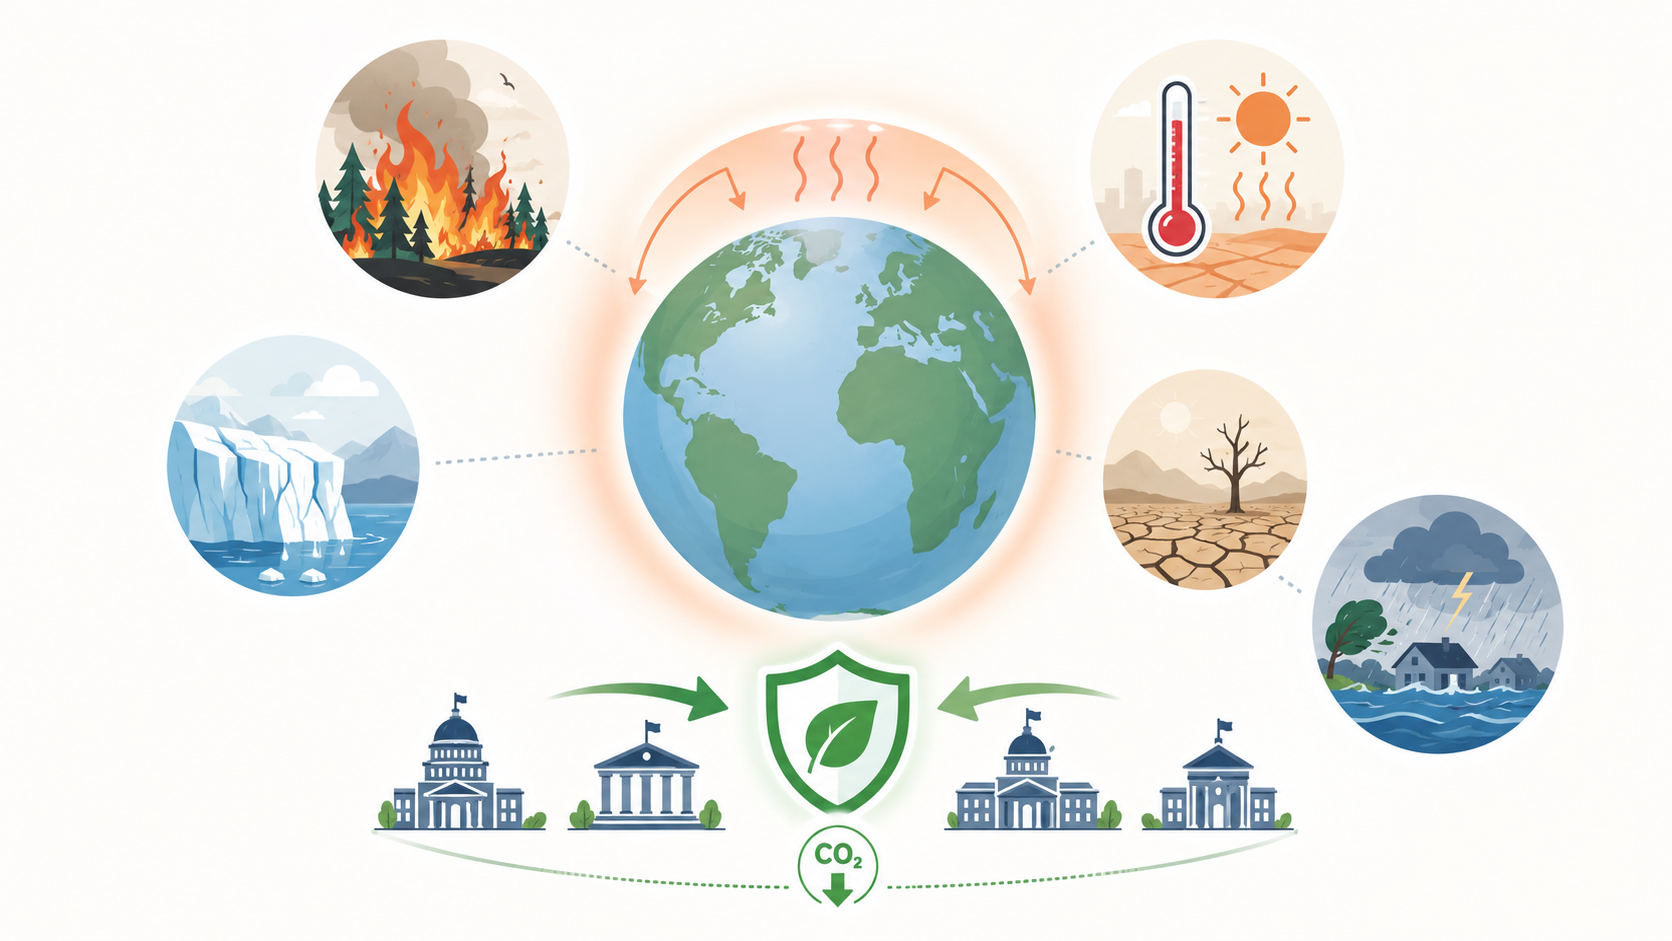
\includegraphics[
        width=1\linewidth,
                trim=15 15 15 15,
        clip
    ]{figures/medioambiente.png}
\end{figure}

\end{frame}


\begin{frame}{Contexto histórico}
\begin{figure}{}
    \centering
    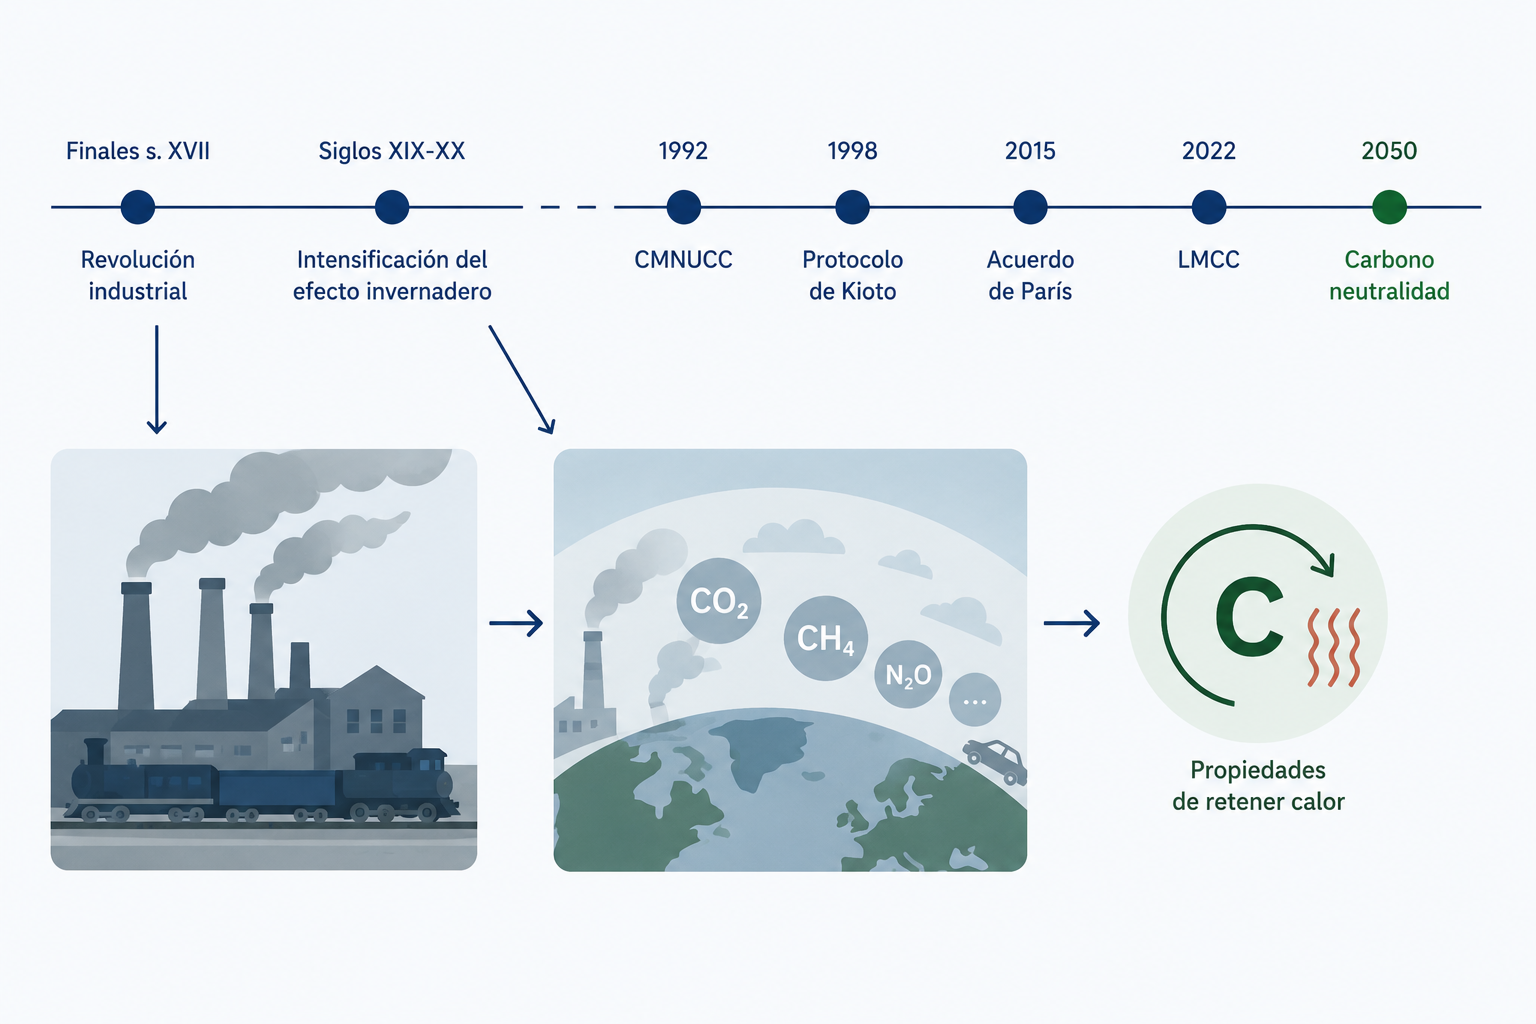
\includegraphics[
        width=1\linewidth,
                trim=15 15 15 15,
        clip
    ]{figures/intro1.png}
\end{figure}

\end{frame}


\begin{frame}{Contexto histórico}
\begin{figure}{}
    \centering
    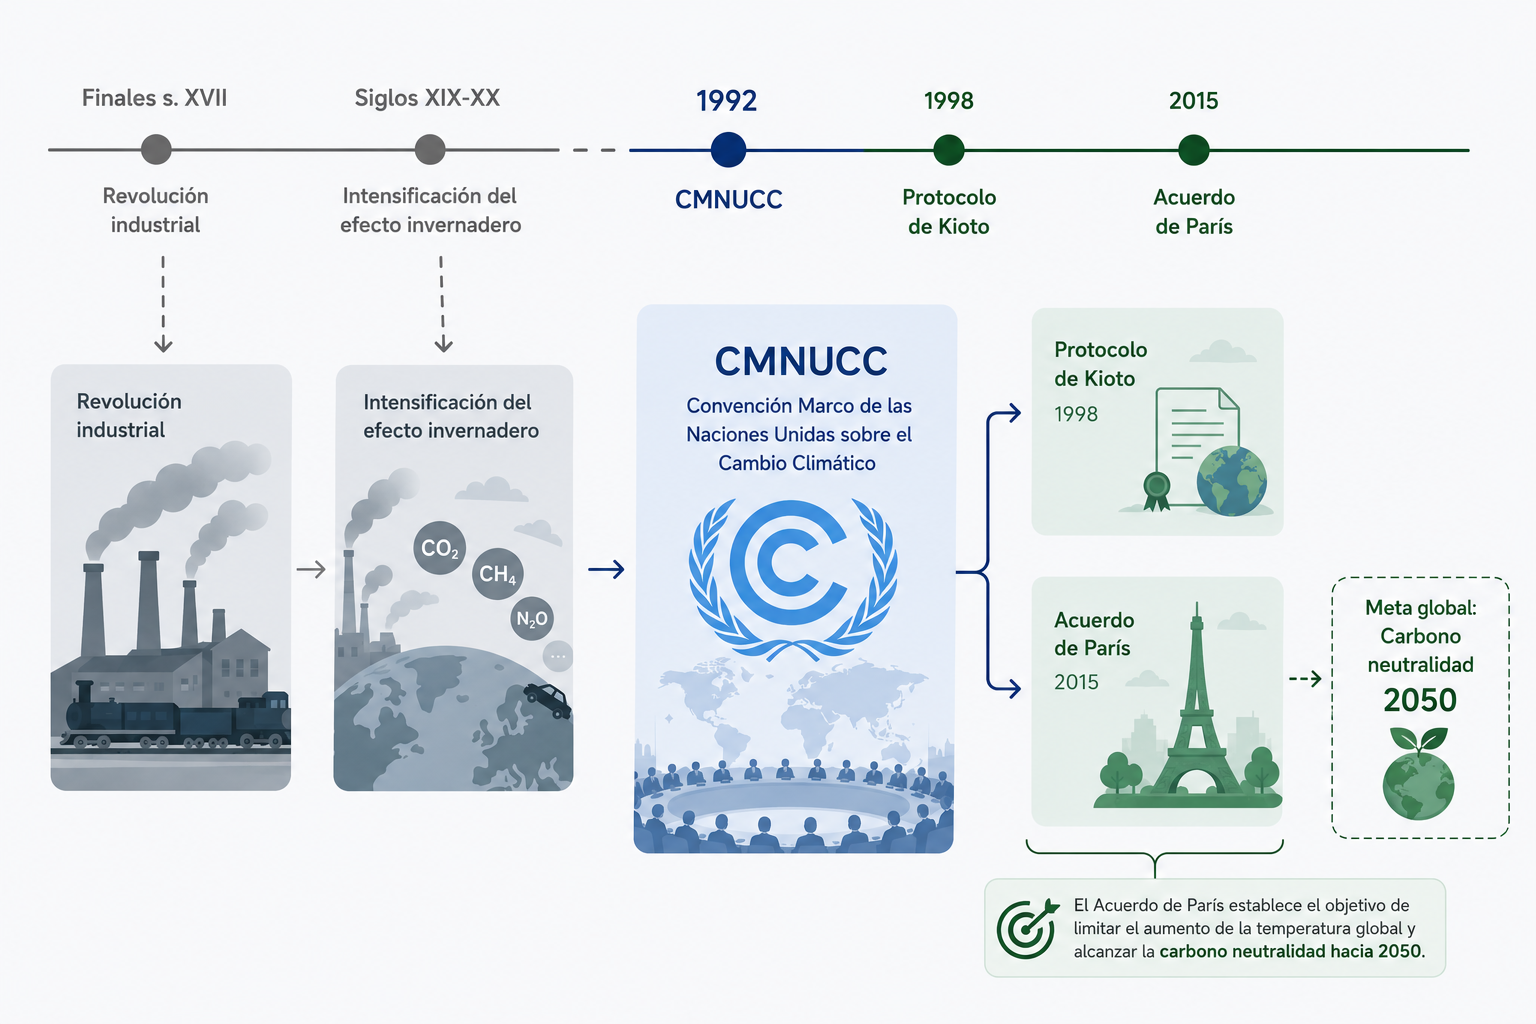
\includegraphics[
        width=1\linewidth,
        trim=15 15 15 15,
        clip
    ]{figures/intro2.png}
\end{figure}

\end{frame}

\begin{frame}{Contexto histórico}
\begin{figure}{}
    \centering
    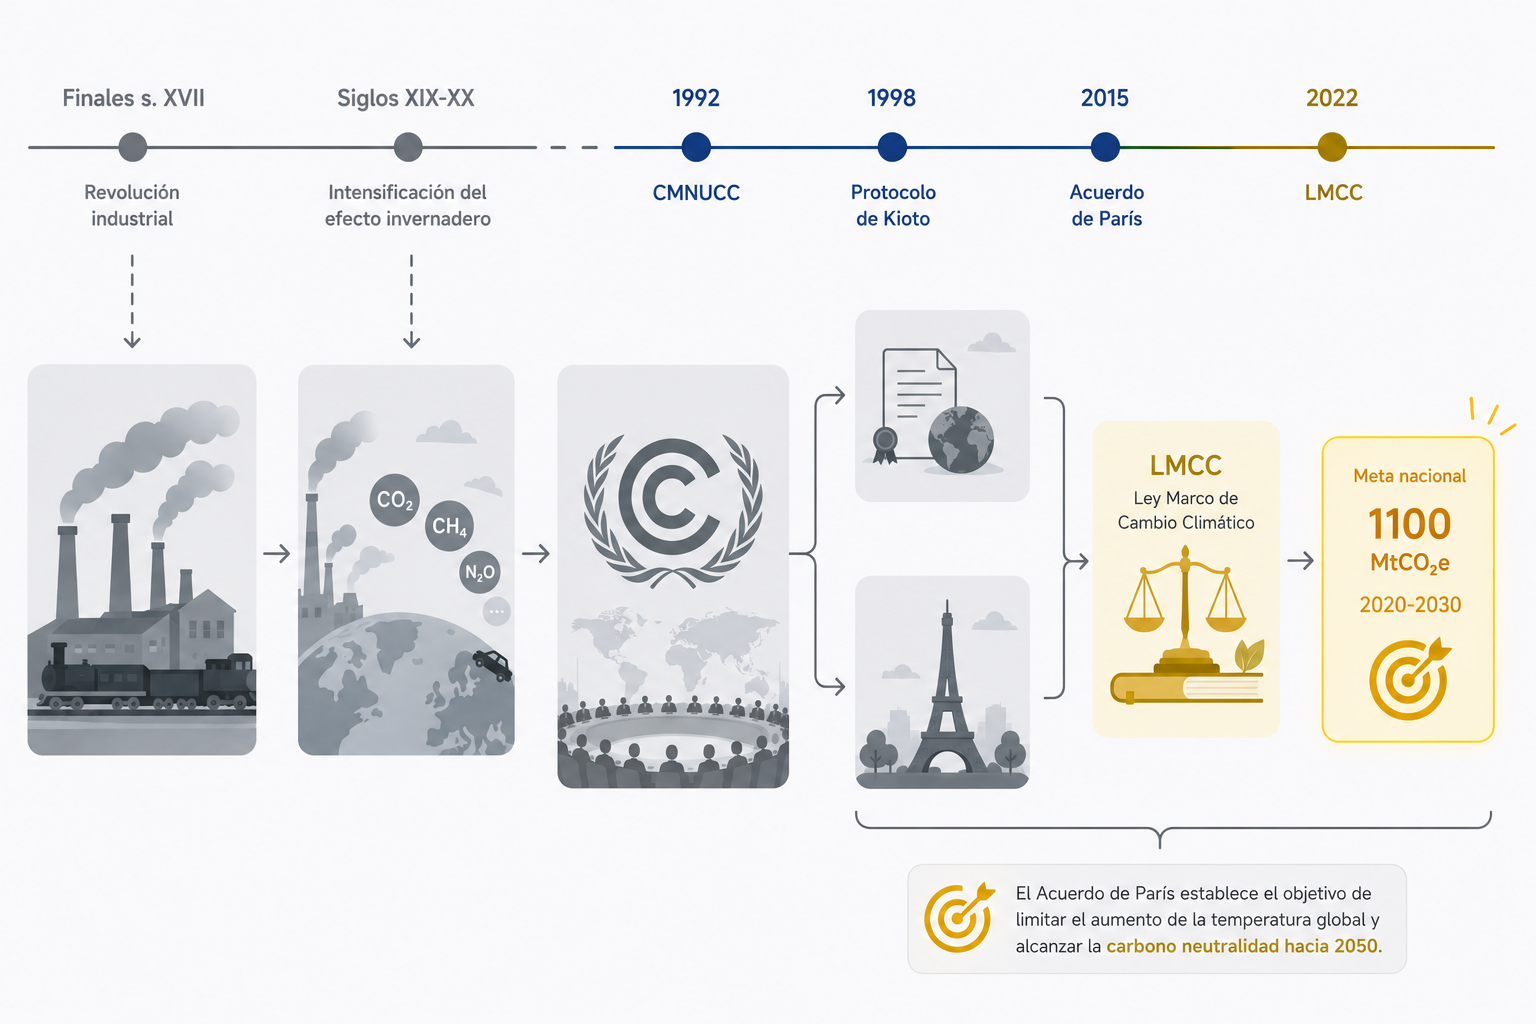
\includegraphics[
        width=1\linewidth,
        trim=15 15 15 15,
        clip
    ]{figures/intro3.png}
\end{figure}

\end{frame}

% \begin{frame}{Trayectoria Climática}
%  \begin{figure}
%     \centering
%     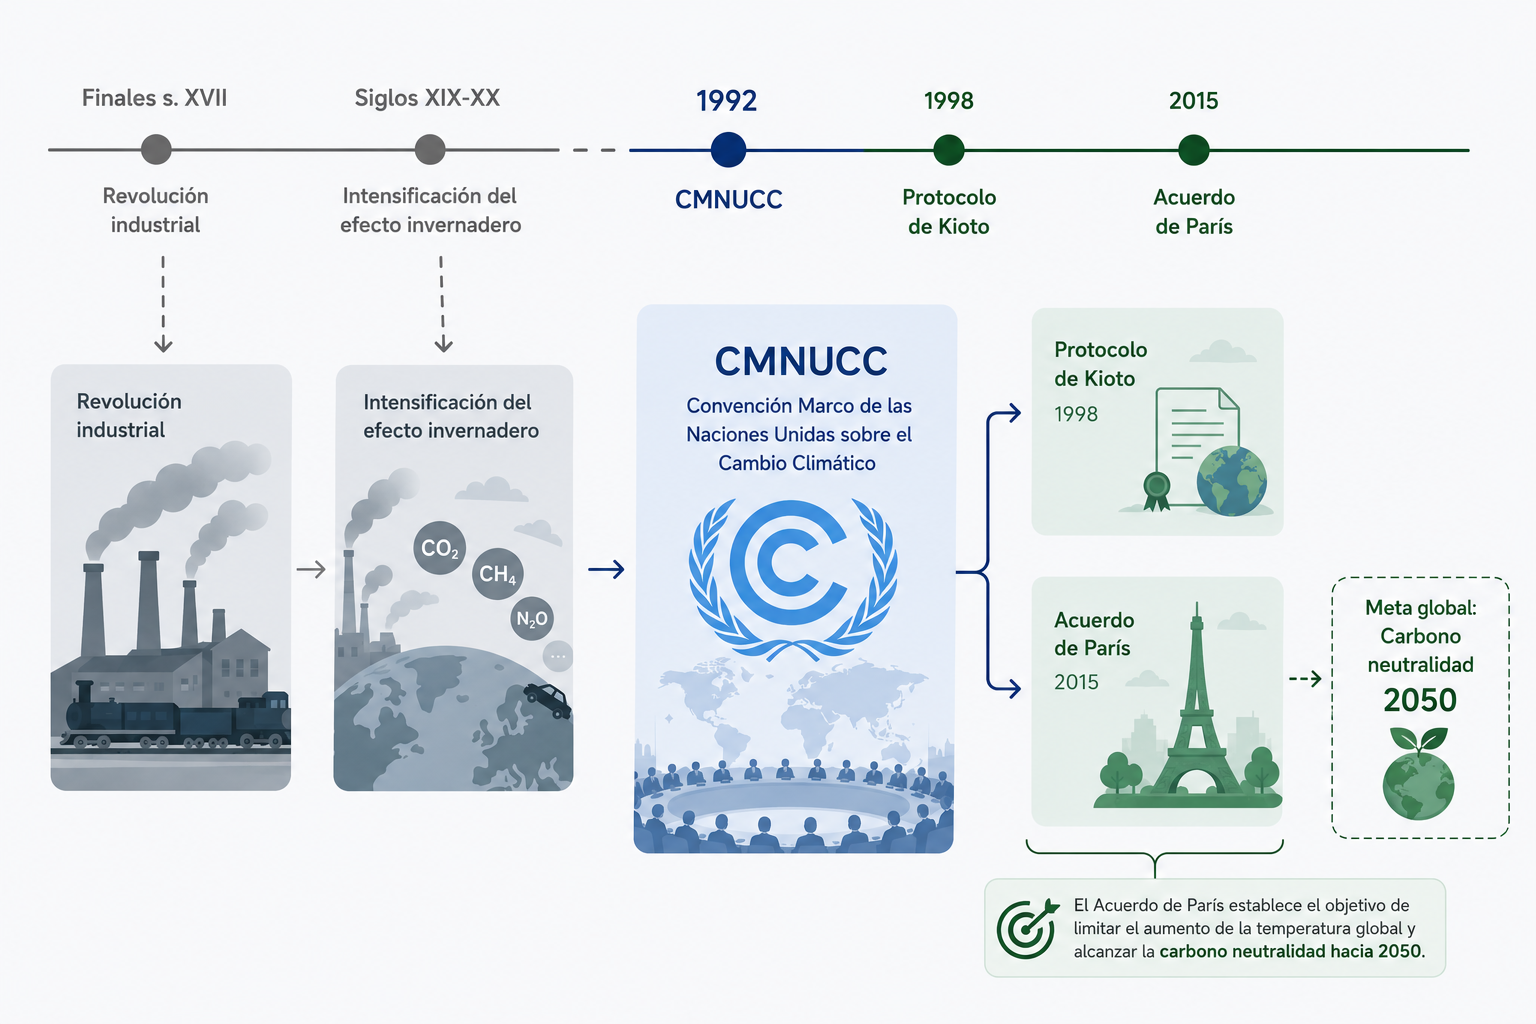
\includegraphics[width=1\linewidth]{figures/intro2.png}
% \end{figure}
   
% \end{frame}

\begin{frame}{Posibilidad de mitigación por ministerio}

\begin{figure}
    \centering
    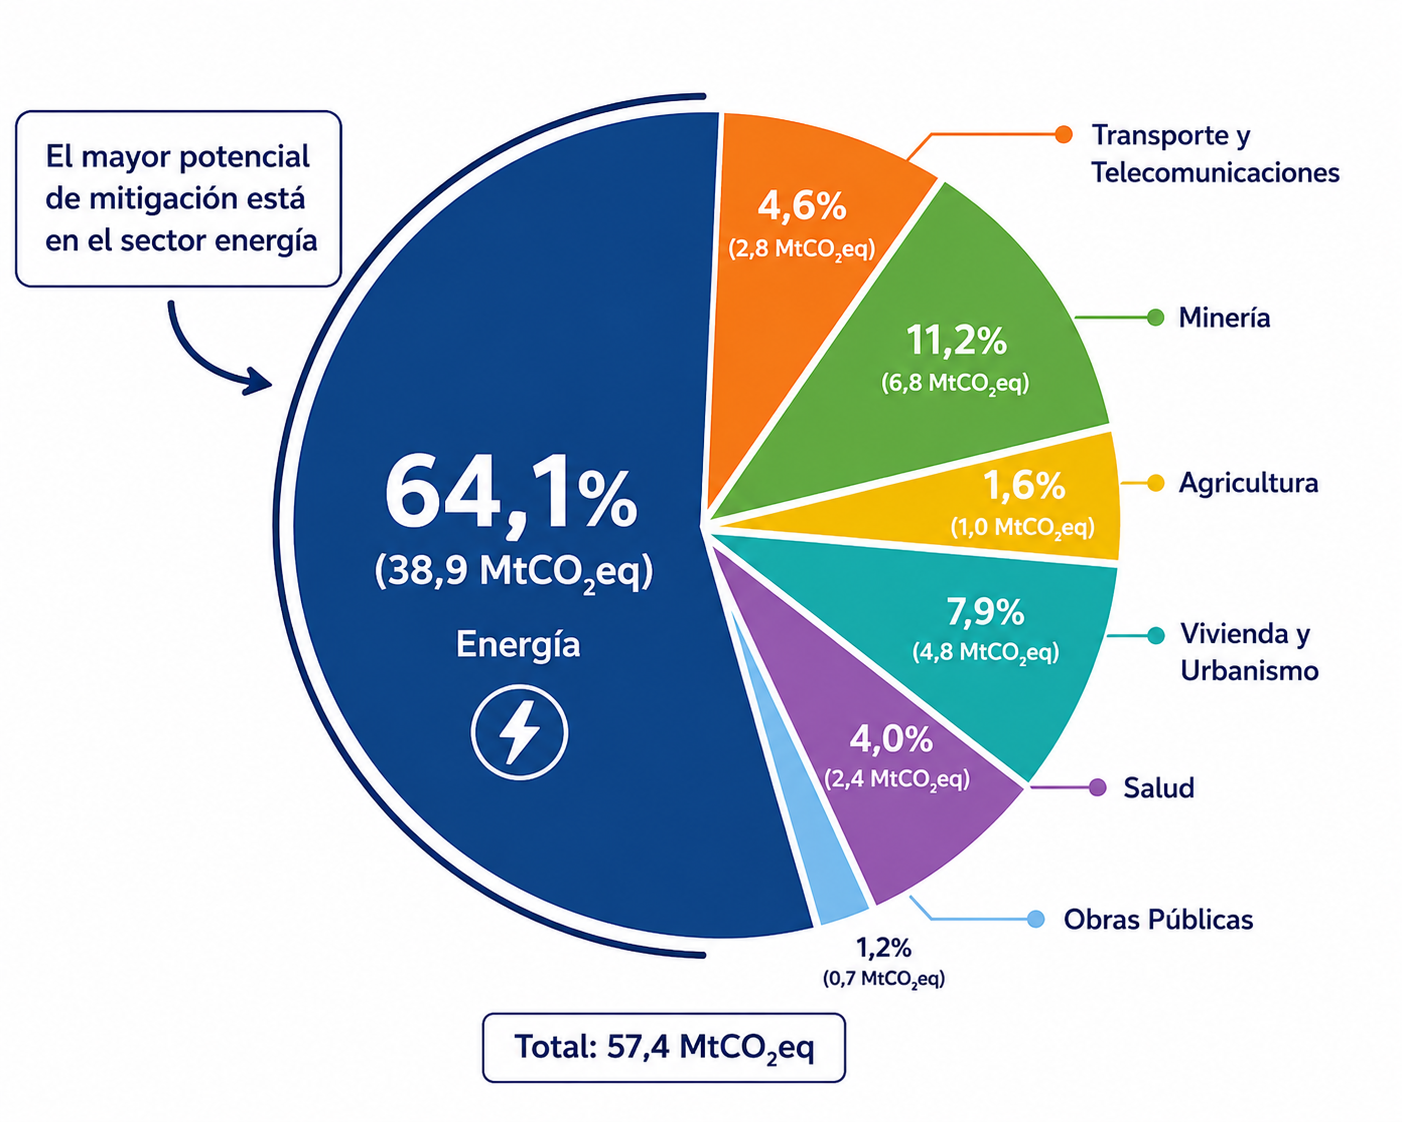
\includegraphics[
        width=0.8\linewidth,
        trim=15 15 15 15,
        clip
    ]{figures/torta mitigacion.png}

\end{figure}
\end{frame}

% --- DIAPOSITIVA 2: PREGUNTA (CENTRADA Y LIMPIA) ---

\begin{frame}[c]{\textit{Pero...}}
    \centering

    \vspace{.7cm}
    
    {\Huge \textbf{¿Está Chile realmente alineado}}
    
    \vspace{0.3cm}
    
    {\Huge \textbf{con sus metas climáticas?}}
\end{frame}



\begin{frame}{Política Climática en Chile}
\begin{figure}
    \centering
    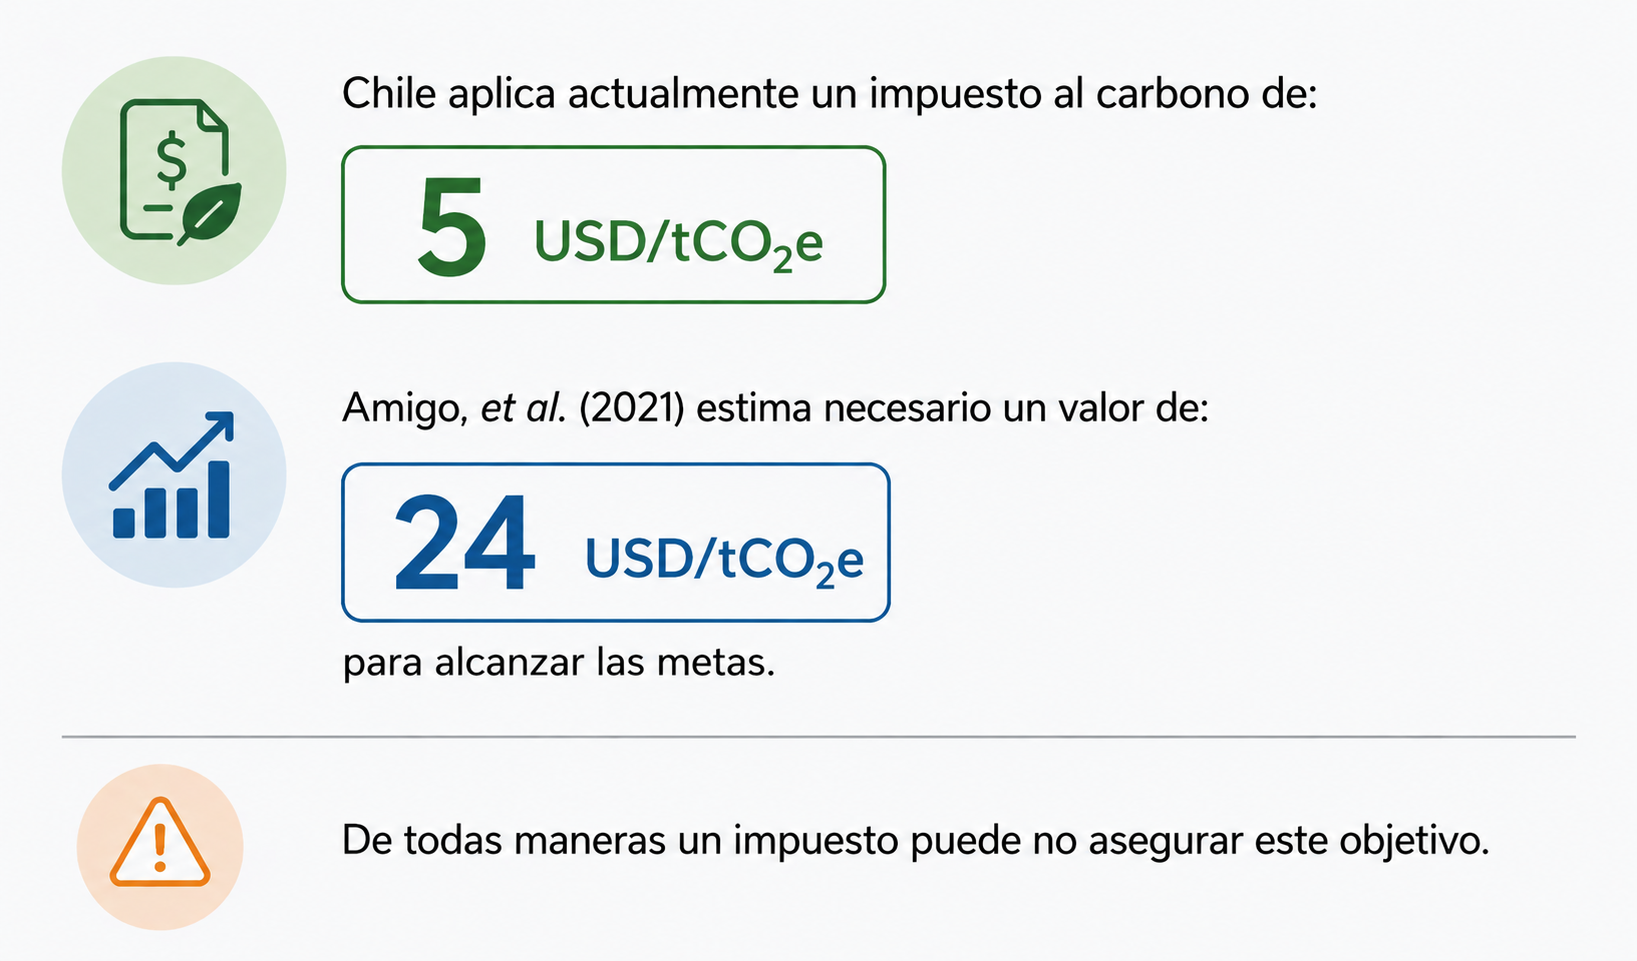
\includegraphics[
        width=0.92\linewidth,
        trim=15 15 15 15,
        clip
    ]{figures/impcarb.png}
\end{figure}
\end{frame}

\begin{frame}{Sistema \textit{Cap-and-Trade} por \cite{amigo_two_2021}}

\vspace{-0.4cm}

\begin{figure}
    \centering
    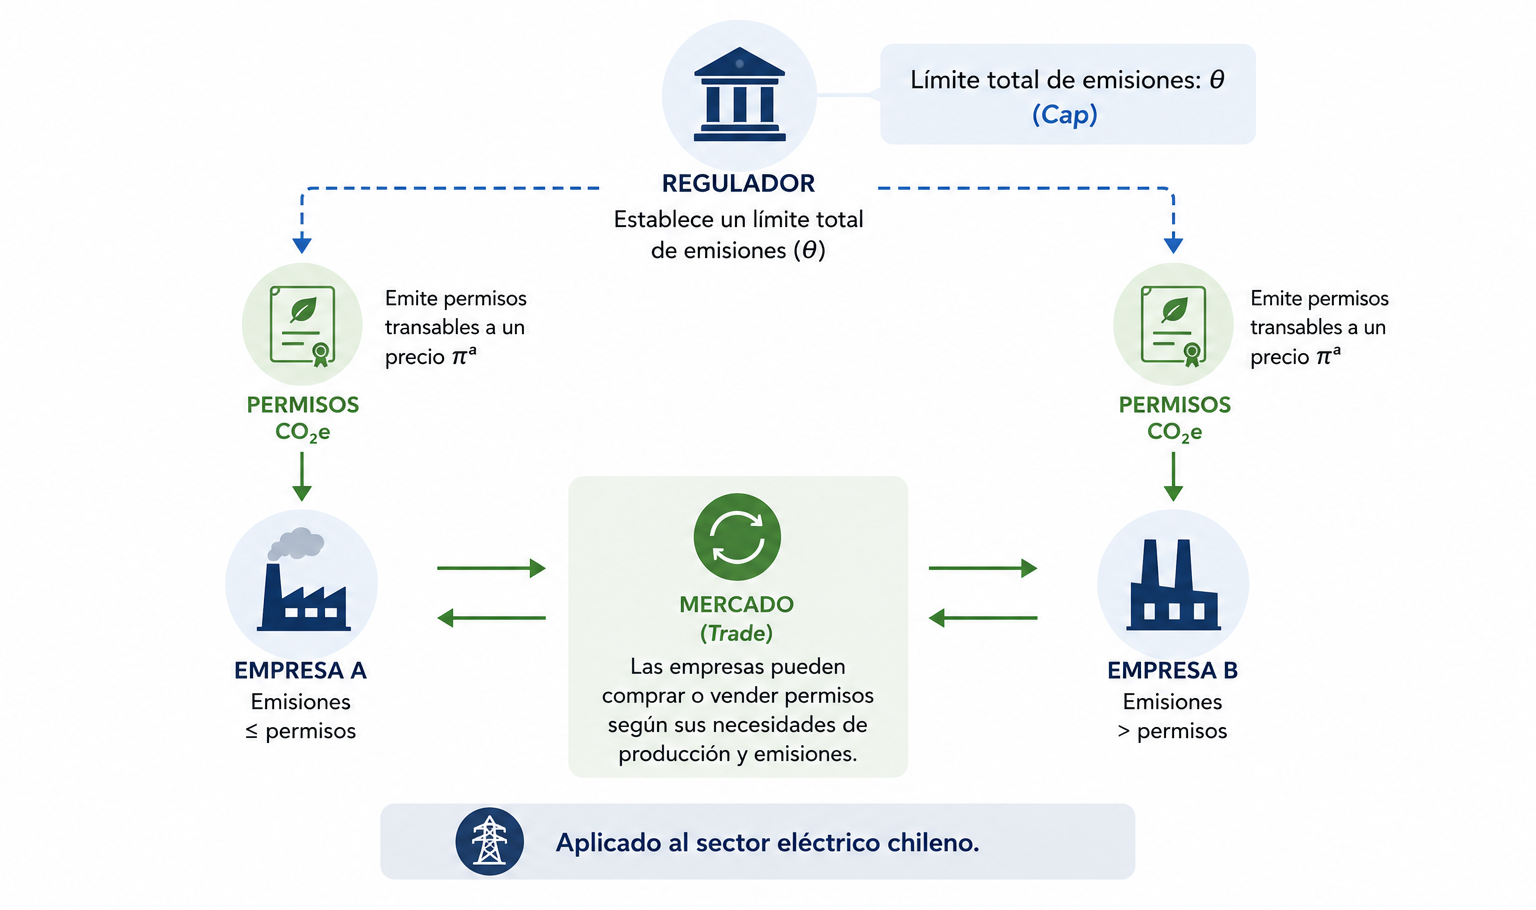
\includegraphics[
        width=1\linewidth,
        trim=15 15 15 15,
        clip
    ]{figures/cap and trade.png}
\end{figure}

\end{frame}


\begin{frame}{El CAP: presupuesto ambiental de emisiones}

\vspace{0cm}

\begin{figure}
    \centering
    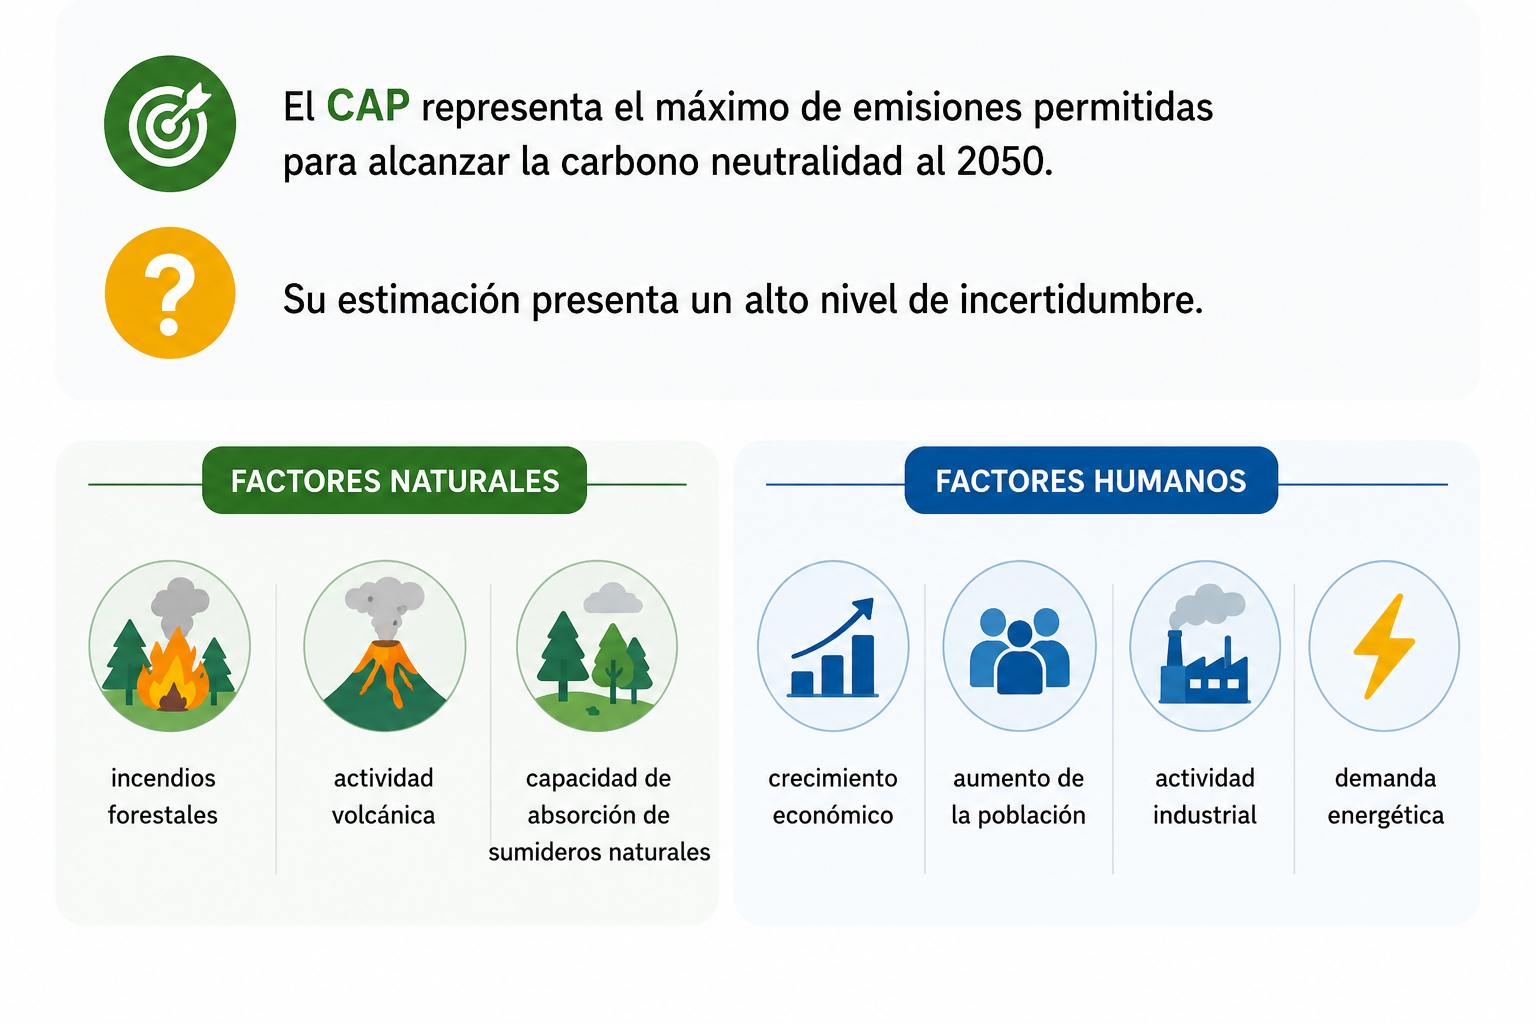
\includegraphics[
        width=1\linewidth,
        trim=1 1 1 1,
        clip
    ]{figures/ELCAP.png}
\end{figure}

\end{frame}


%\vspace{-0.4cm}

\begin{frame}{Limitaciones del modelo \cite{amigo_two_2021}}

\vspace{0.4cm}
\filaIcono{SoftBlue}{\faIcon{file-alt}}{El modelo supone \textbf{información perfecta} sobre el presupuesto de emisiones.}

\vspace{0.35cm}
\filaIcono{ClimateGreen}{\faDollarSign}{Un \textbf{costo social} sin definición ni uso al modelar.}

\end{frame}



\begin{frame}{Objetivo del trabajo}

\begin{tcolorbox}[tarjeta=DeepBlue, title={\faBullseye\ \ Objetivo general}]
\centering
Modelar un planificador racional con \textbf{atención limitada}, junto con una
\textbf{función penalizadora} por alejarse del $CAP$, en un sistema de
\emph{cap-and-trade}.
\end{tcolorbox}

\vspace{0.3cm}
\begin{columns}[T]
\begin{column}{0.48\textwidth}
  \filaIcono{DeepBlue}{\faBolt}{\textbf{Foco:} sector eléctrico chileno.}
\end{column}
\begin{column}{0.48\textwidth}
  \filaIcono{DeepBlue}{\faIcon{calendar-alt}}{\textbf{Periodo:} \valHorizonte.}
\end{column}
\end{columns}

\end{frame}




\begin{frame}{Simbología del modelo}

\vspace{-0.1cm}
\begin{columns}[T]
\begin{column}{0.24\textwidth}\tarjetaSimbolo{ClimateGreen}{\faChartArea}{CAP}{\descCAP\\$\distCAP$}{\unidadMt}\end{column}
\begin{column}{0.24\textwidth}\tarjetaSimbolo{SoftBlue}{\faBroadcastTower}{CAP_s}{\descCAPs}{\unidadMt}\end{column}
\begin{column}{0.24\textwidth}\tarjetaSimbolo{DeepBlue}{\faAnchor}{CAP_d}{\descCAPd}{\unidadMt}\end{column}
\begin{column}{0.24\textwidth}\tarjetaSimbolo{MediumGray}{\faWaveSquare}{\varepsilon}{\descEps\\$\distEps$}{\unidadMt}\end{column}
\end{columns}

\vspace{0.25cm}
\begin{columns}[T]
\begin{column}{0.06\textwidth}\end{column}
\begin{column}{0.28\textwidth}\tarjetaSimbolo{ClimateGreen}{\faClipboardCheck}{\theta}{\descTheta}{\unidadMt}\end{column}
\begin{column}{0.28\textwidth}\tarjetaSimbolo{ClimateRed}{\faTag}{\pi^a}{\descPiA}{\unidadUSDt}\end{column}
\begin{column}{0.28\textwidth}\tarjetaSimbolo{DeepBlue}{\faUsers}{\kappa}{\descKappa}{\unidadUSDt}\end{column}
\begin{column}{0.06\textwidth}\end{column}
\end{columns}

\end{frame}

\begin{frame}{Planificador social con inatención conductual}

\vspace{-0.15cm}
\begin{center}
\begin{tcolorbox}[tarjeta=DeepBlue, width=0.92\linewidth]
\centering $\displaystyle \ecThetaOptimo$
\end{tcolorbox}
\end{center}

\vspace{-0.15cm}
\begin{center}
\begin{tikzpicture}[font=\scriptsize]
  % eje de atención
  \draw[-latex, very thick, draw=SoftBlue] (-3.6,2.05) -- (3.6,2.05);
  \fill[SoftBlue] (-3.6,2.05) circle (1.6pt);
  \node[above=1pt] at (0,2.05) {Nivel de atención $m$};
  \node[below=2pt, DeepBlue] at (-3.6,2.05) {$0$};
  \node[below=2pt, ClimateGreen] at (3.6,2.05) {$1$};
  \node[left=2pt, DeepBlue, align=center] at (-3.75,2.05) {Atención baja\\$CAP_d$};
  \node[right=2pt, ClimateGreen, align=center] at (3.75,2.05) {Atención alta\\$CAP_s$};
  % entradas
  \node[caja=DeepBlue] (ancla) at (-3.1,0.55) {Valor por defecto (ancla)\\[1pt] $CAP_d$};
  \node[caja=ClimateGreen] (senal) at (3.1,0.55) {Señal observada (ruidosa)\\[1pt] $\ecSenal$};
  \node[caja=MediumGray] (sesgo) at (3.3,-1.35) {Sesgo económico\\[1pt] $\dfrac{\pi^a}{\kappa}$};
  % planificador
  \node[circle, draw=DeepBlue, very thick, fill=white, minimum size=1.5cm,
        align=center, text=DeepBlue] (plan) at (0,-1.05) {Planificador\\social};
  % salida
  \node[draw=DeepBlue, thick, rounded corners=3pt, fill=SkyBlue,
        align=center, inner sep=4pt] (out) at (0,-2.85)
        {Permisos emitidos\ \ $\theta^*$};
  % flechas
  \draw[flecha=DeepBlue] (ancla.south) to[out=-70,in=170] (plan.west);
  \draw[flecha=ClimateGreen] (senal.south) to[out=-110,in=10] (plan.east);
  \draw[flecha=MediumGray, dashed] (sesgo.west) -- (plan.east);
  \draw[flecha=DeepBlue] (plan.south) -- (out.north);
\end{tikzpicture}
\end{center}

\end{frame}



% \begin{frame}{}
% \begin{figure}{}
%     \centering
%     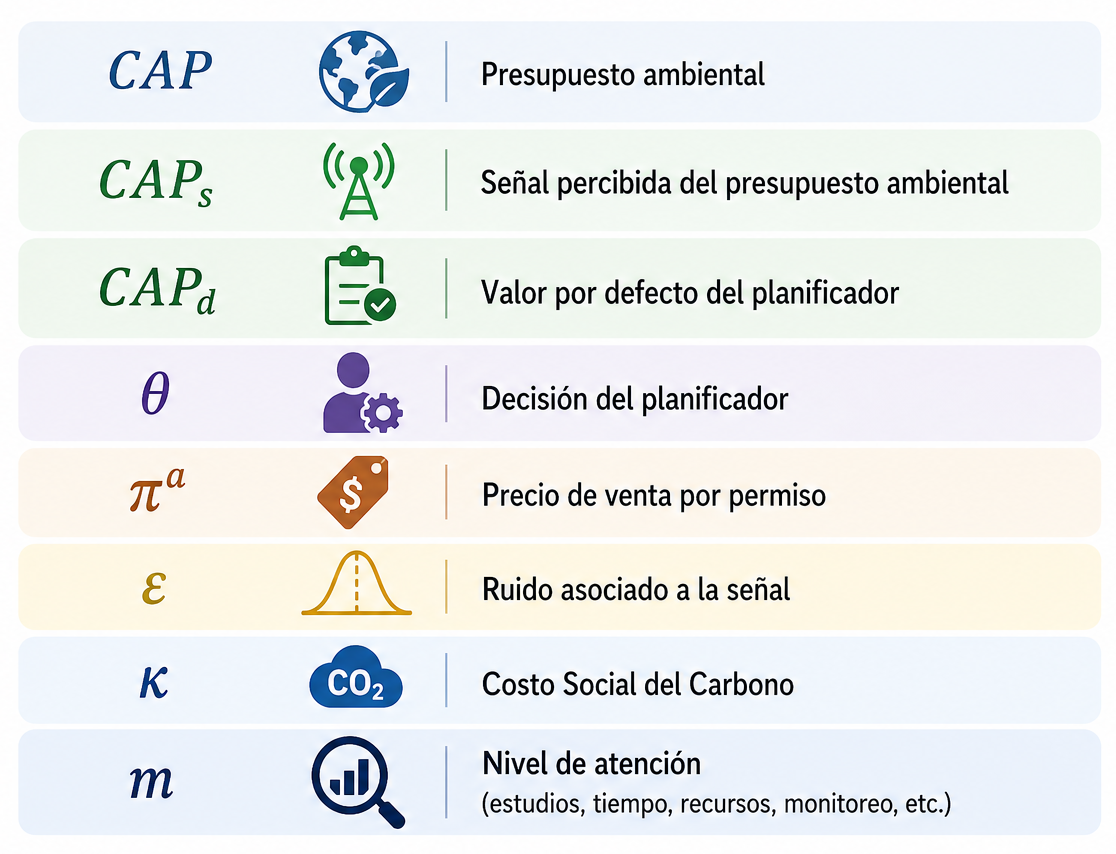
\includegraphics[
%         width=0.9\linewidth,
%         trim=15 15 15 15,
%         clip
%     ]{figures/parametros8.png}
% \end{figure}

% \end{frame}


% \begin{frame}{Modelar el presupuesto ambiental}
% \begin{figure}{}
%     \centering
%     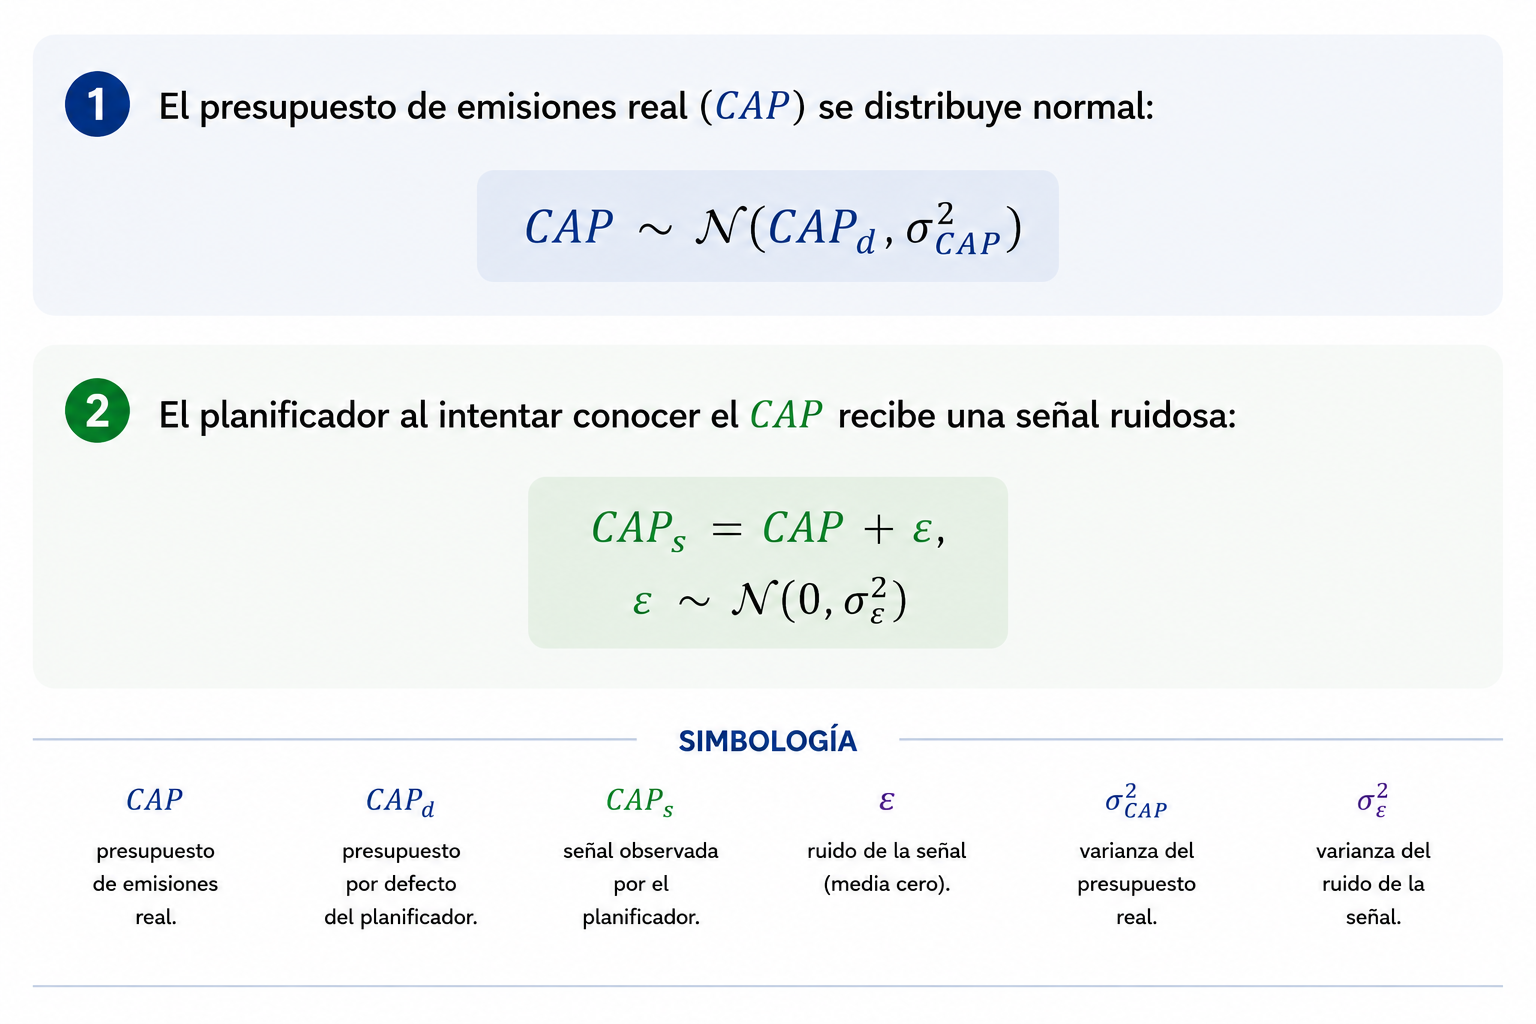
\includegraphics[
%         width=1\linewidth,
%                 trim=15 15 15 15,
%         clip
%     ]{figures/modelacion.png}
% \end{figure}

% \end{frame}






% \begin{frame}{Función de beneficio del planificador}
% \begin{figure}{}
%     \centering
%     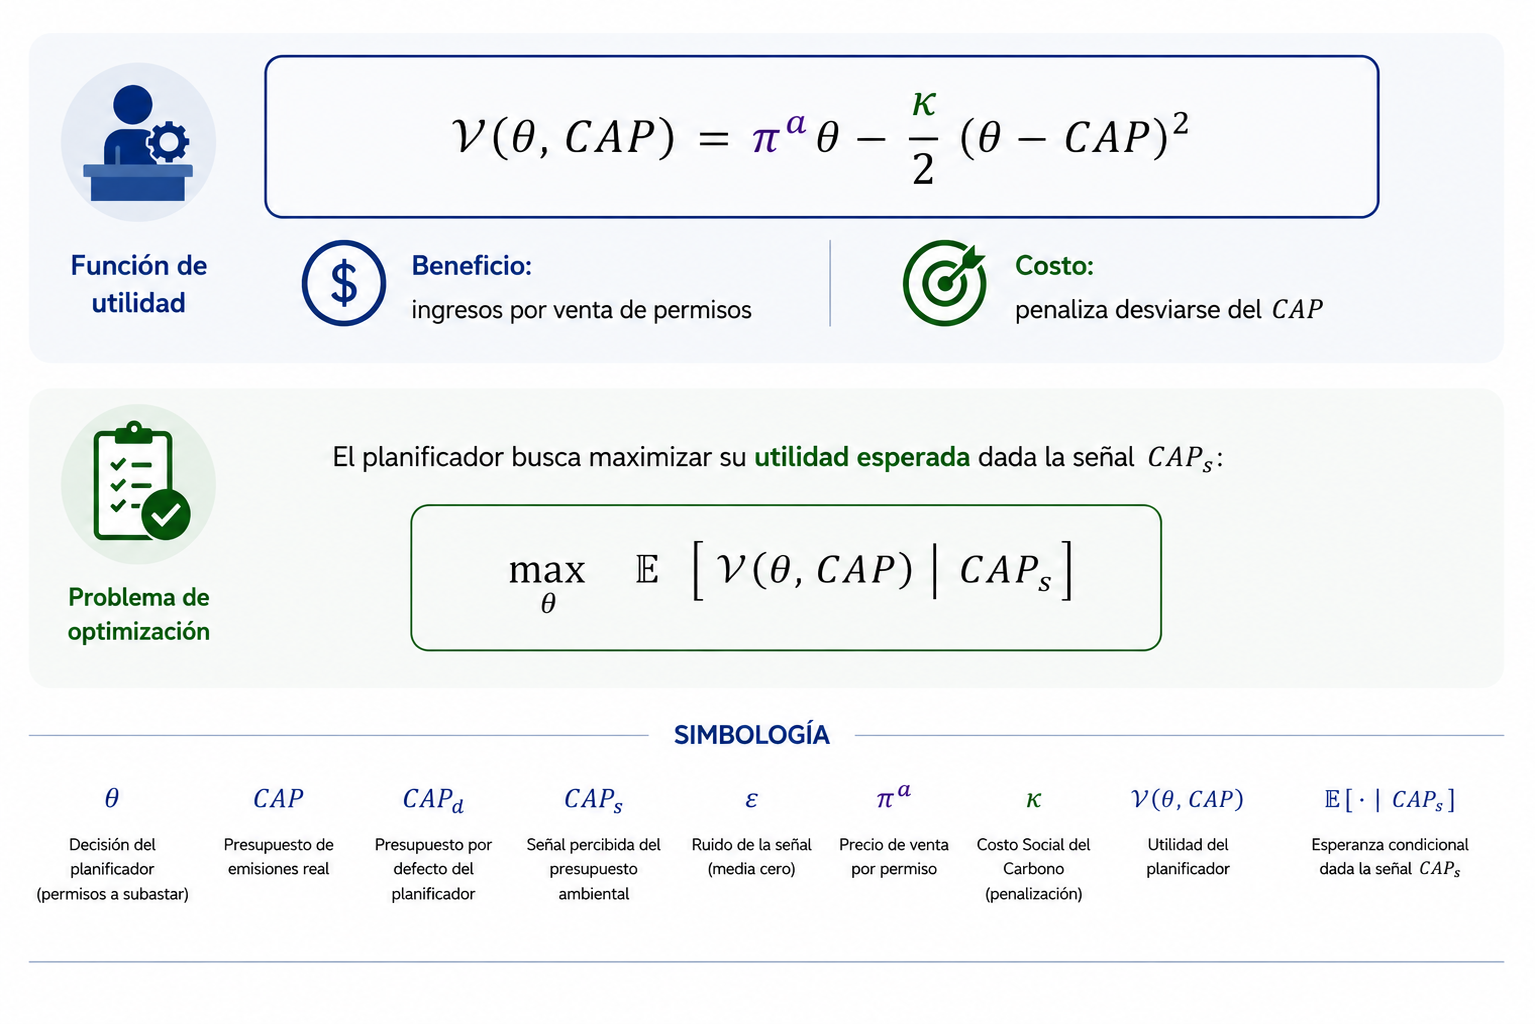
\includegraphics[
%         width=1\linewidth,
%         trim=15 15 15 15,
%         clip
%     ]{figures/modelo2.png}
% \end{figure}
% \end{frame}


% \begin{frame}{Decisión óptima del planificador}
% \begin{figure}{}
%     \centering
%     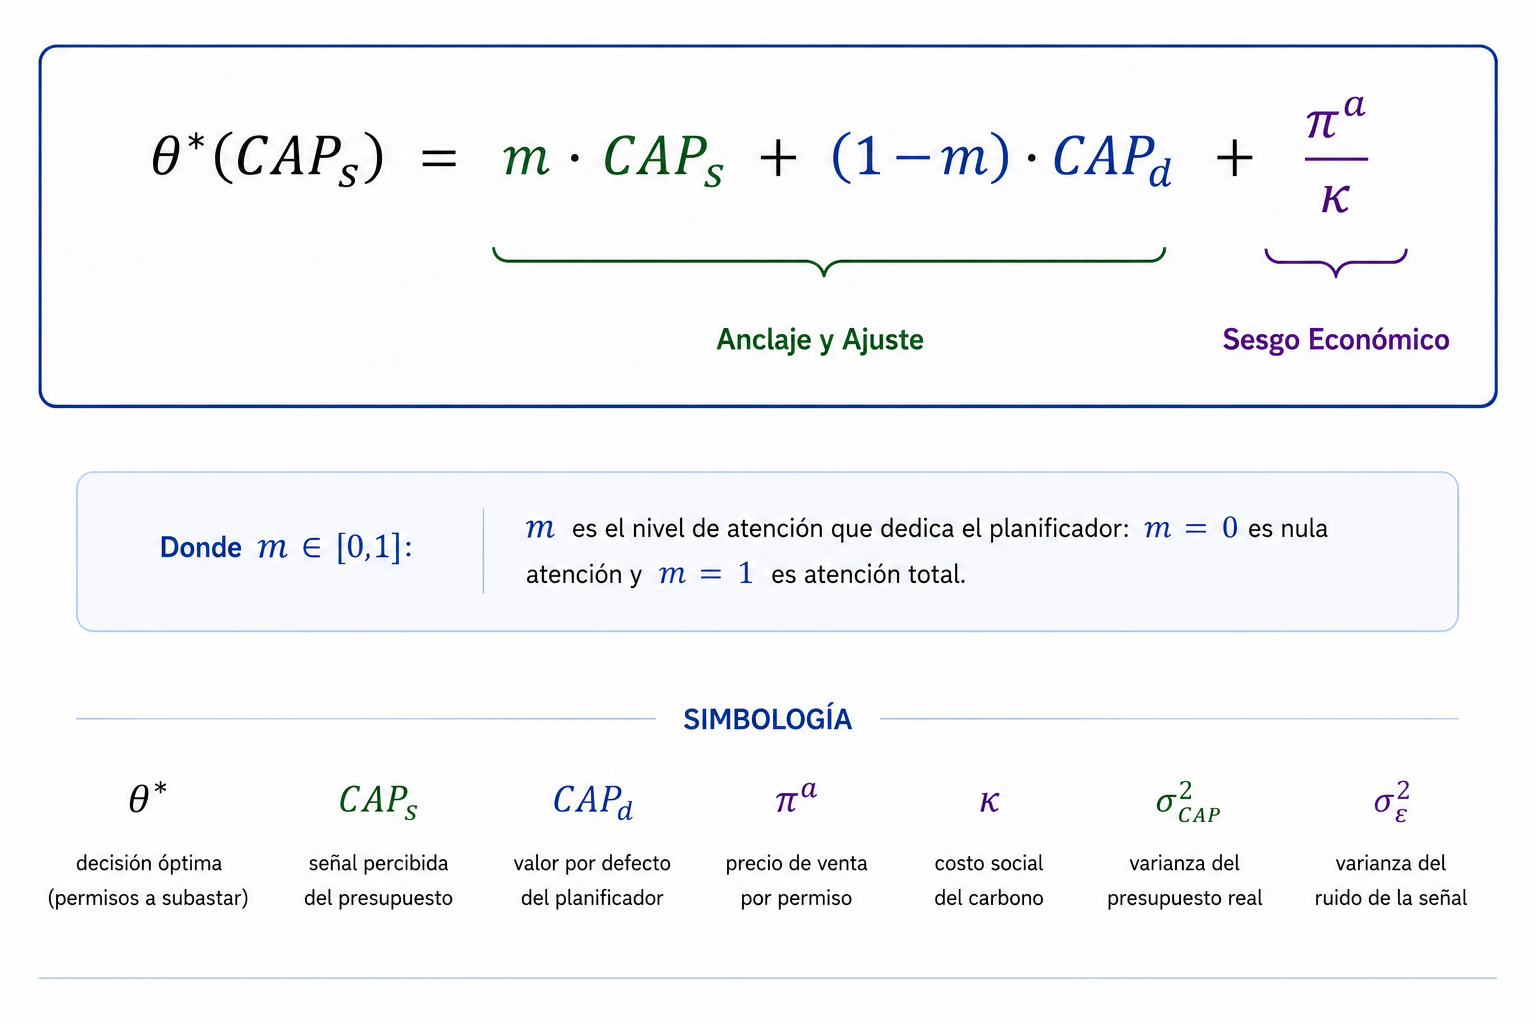
\includegraphics[
%         width=1\linewidth,
%         trim=15 15 15 15,
%         clip
%     ]{figures/modelo1.png}
% \end{figure}

% \end{frame}


\begin{frame}{Parámetros para Chile}

\vspace{0.15cm}
\filaIcono{ClimateGreen}{\faBullseye}{$CAP_s = \valCAPs$ \unidadMt \hfill {\scriptsize \origenCAPs}}

\vspace{0.15cm}
\filaIcono{DeepBlue}{\faBalanceScale}{$CAP_d = \valCAPd$ \unidadMt \hfill {\scriptsize \origenCAPd}}

\vspace{0.15cm}
\filaIcono{MediumGray}{\faChartArea}{$\sigma_{CAP} = \valSigmaCAP$ \unidadMt \hfill {\scriptsize \origenSigmaCAP}}

\vspace{0.15cm}
\filaIcono{ClimateRed}{\faDollarSign}{$\kappa = \valKappa$ \unidadUSDt \hfill {\scriptsize \origenKappa}}

\vspace{0.2cm}
{\tiny\color{MediumGray} Mismos valores que el cuadro de parámetros base de la memoria: ambos leen \texttt{shared/datos-modelo.tex}.}

\end{frame}


\begin{frame}{¿Qué nivel de atención tiene el planificador en Chile?}

\vspace{0.1cm}
\begin{tcolorbox}[tarjeta=ClimateGreen, title={\faBullseye\ \ 1. Metodología de ajuste}]
\begin{columns}[c]
\begin{column}{0.32\textwidth}\centering{\color{ClimateGreen}\faIcon{calendar-alt}}\\{\scriptsize Matriz real 2024}\end{column}
\begin{column}{0.32\textwidth}\centering{\color{ClimateGreen}\faLayerGroup}\\{\scriptsize Matrices modeladas 2024}\end{column}
\begin{column}{0.32\textwidth}\centering{\color{ClimateGreen}\faUsers}\\{\scriptsize 11 escenarios de atención}\end{column}
\end{columns}
\end{tcolorbox}

\vspace{0.1cm}
\begin{tcolorbox}[tarjeta=SoftBlue, title={\faSearch\ \ 2. Comparación}]
\centering{\scriptsize Comparar \ \ $\rightarrow$ \ \ buscar mejor ajuste \ \ $\rightarrow$ \ \ menor distancia absoluta}
\end{tcolorbox}

\vspace{0.1cm}
\begin{tcolorbox}[tarjeta=DeepBlue, title={\faChartBar\ \ 3. Resultado clave}]
\centering
{\faCheckCircle}\ \ Mínimo en $m = 0$ \quad$\Rightarrow$\quad \textbf{planificador inatento}
\end{tcolorbox}

\end{frame}


\begin{frame}{Implementación}

\vspace{0.3cm}
\filaIcono{ClimateGreen}{\faPuzzlePiece}{\textbf{Modelo de complementariedad mixta:} formulación matemática que modela el equilibrio del sistema.}

\vspace{0.3cm}
\filaIcono{DeepBlue}{\faCogs}{\textbf{PATH:} solver especializado para resolver problemas de complementariedad.}

\vspace{0.3cm}
\filaIcono{MediumGray}{\faCode}{\textbf{Julia + JuMP:} implementación flexible y eficiente del modelo.}

\end{frame}




\begin{frame}{Incertidumbre por nivel de atención}

\centering

\vspace{-0.1cm}

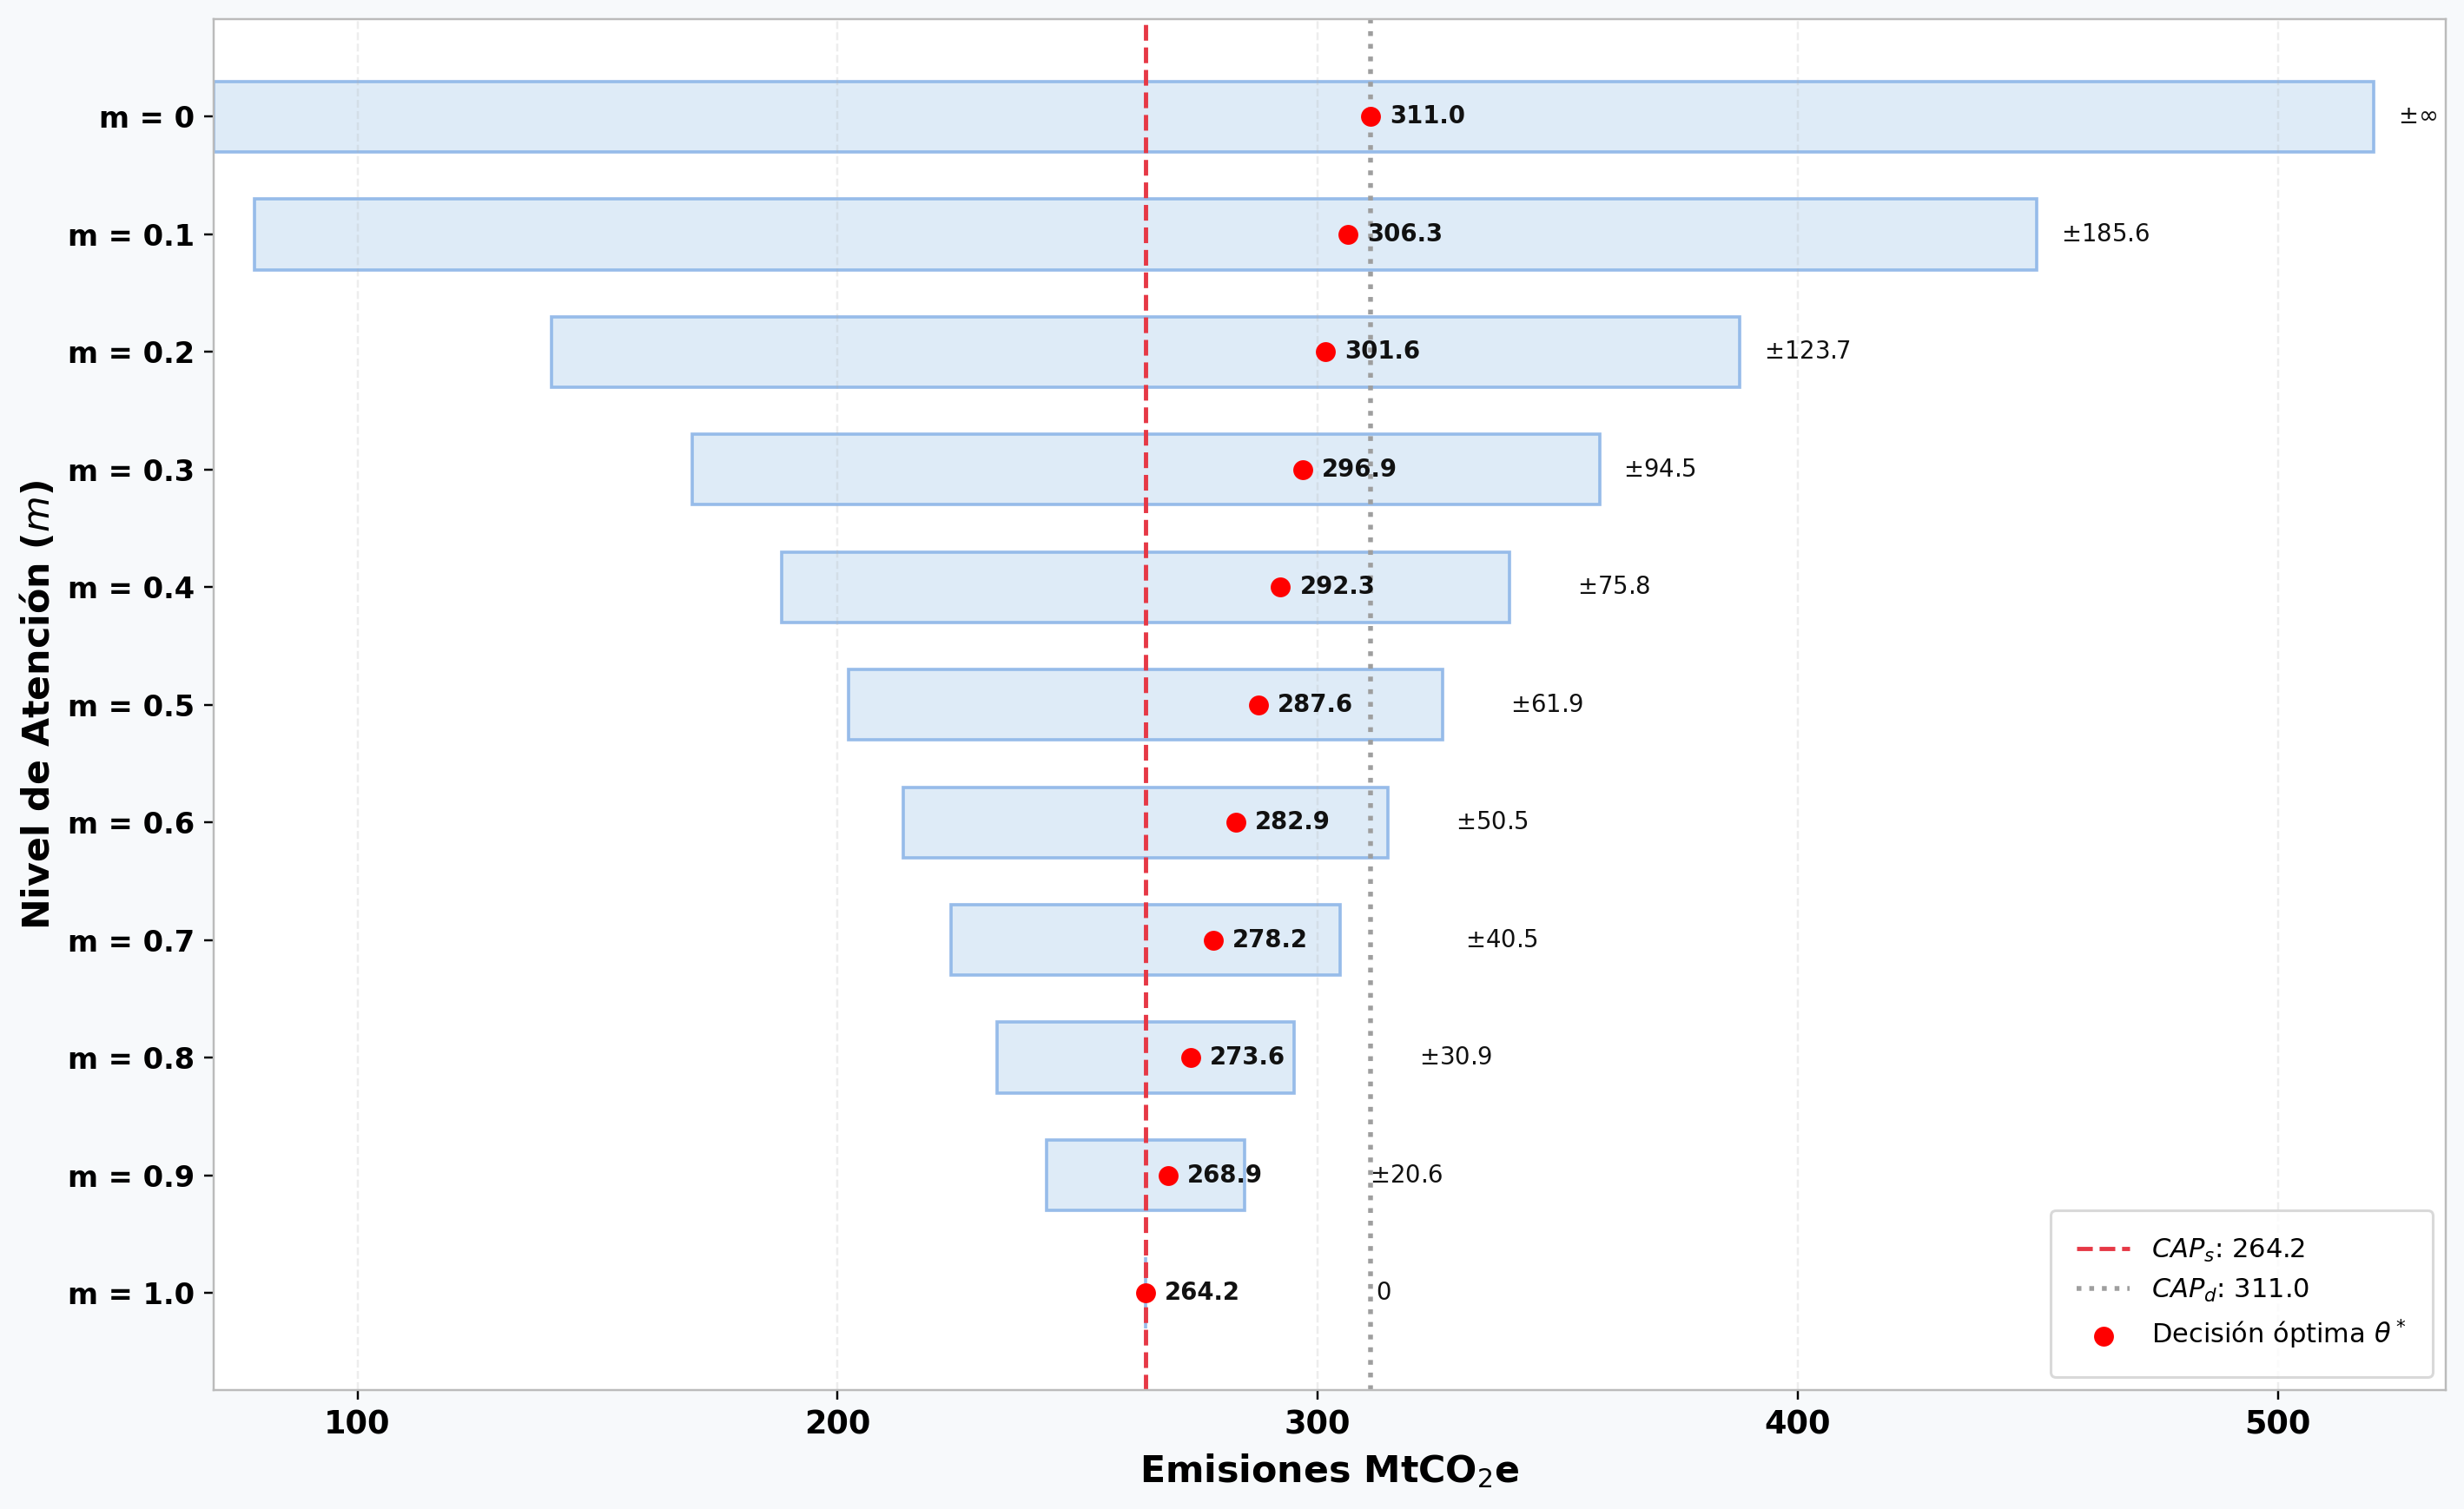
\includegraphics[
    width=0.98\textwidth,
    height=0.78\textheight,
    keepaspectratio
]{figures/bmbudo.png}

\vspace{0.05cm}

{\tiny
\begin{tcolorbox}[
    colback=white,
    colframe=SoftBlue,
    arc=1.5mm,
    boxrule=0.5pt,
    hbox,
    left=2pt,
    right=2pt,
    top=1pt,
    bottom=1pt
]
\centering
\textbf{Fórmulas usadas:}
\(
CAP_s = CAP + \epsilon
\qquad
CAP = CAP_s \pm \sigma_{\epsilon}
\)
\end{tcolorbox}
}

\end{frame}


% \begin{frame}{Casos Límites}

%     \begin{center}
%         {\Large $CAP_s = CAP + \epsilon$}       
%         {\Large $CAP = CAP_s \pm \sigma_{\epsilon}$}
%     \end{center}

%     \vspace{0.8cm}

% \end{frame}


% \begin{frame}{Resultados Caso Límite $CAP_s +\sigma_\varepsilon$}

% \begin{table}[H]
% \centering
% \caption{Resultados del modelo según nivel de atención $m$}
% \label{tab:resultados_m}

% \renewcommand{\arraystretch}{1.2}
% \setlength{\tabcolsep}{5pt}

% \resizebox{0.9\textwidth}{!}{%
% \begin{tabular}{cccc}
% \toprule
% $m$ & $\theta$ (MtCO$_2$e) & $CAP$ (MtCO$_2$e) & Beneficio (M USD) \\
% \midrule

% 0,0 & 311,0 & N/A & N/A \\

% 0,2 & 301,6 & 387,92 & $-2{,}396 \times 10^{11}$ \\

% 0,4 & 292,3 & 339,96 & $-7{,}319 \times 10^{10}$ \\

% 0,6 & 282,9 & 314,71 & $-3{,}253 \times 10^{10}$ \\

% 0,8 & 273,6 & 295,13 & $-1{,}498 \times 10^{10}$ \\

% 1,0 & 264,2 & 264,20 & $5{,}251 \times 10^{4}$ \\

% \bottomrule
% \end{tabular}%
% }

% \end{table}

% \end{frame}


% \begin{frame}{Resultados Caso Límite $CAP_s-\sigma_\epsilon$}

% \begin{table}[H]
% \centering
% \caption{Resultados del modelo según nivel de atención $m$}
% \label{tab:resultados_m_2}

% \renewcommand{\arraystretch}{1.2}
% \setlength{\tabcolsep}{5pt}

% \resizebox{0.9\textwidth}{!}{%
% \begin{tabular}{cccc}
% \toprule
% $m$ & $\theta$ (MtCO$_2$e) & $CAP$ (MtCO$_2$e) & Beneficio (M USD) \\
% \midrule

% 0,0 & 311,0 & N/A & N/A \\

% 0,2 & 301,6 & 140,48 & $-8{,}364 \times 10^{11}$ \\

% 0,4 & 292,3 & 188,44 & $-3{,}473 \times 10^{11}$ \\

% 0,6 & 282,9 & 213,69 & $-1{,}543 \times 10^{11}$ \\

% 0,8 & 273,6 & 233,27 & $-5{,}228 \times 10^{10}$ \\

% 1,0 & 264,2 & 264,20 & $5{,}251 \times 10^{4}$ \\

% \bottomrule
% \end{tabular}%
% }

% \end{table}

% \end{frame}


\begin{frame}{Utilidad en Casos Límite de Incertidumbre}

\centering

\vspace{-0.1cm}

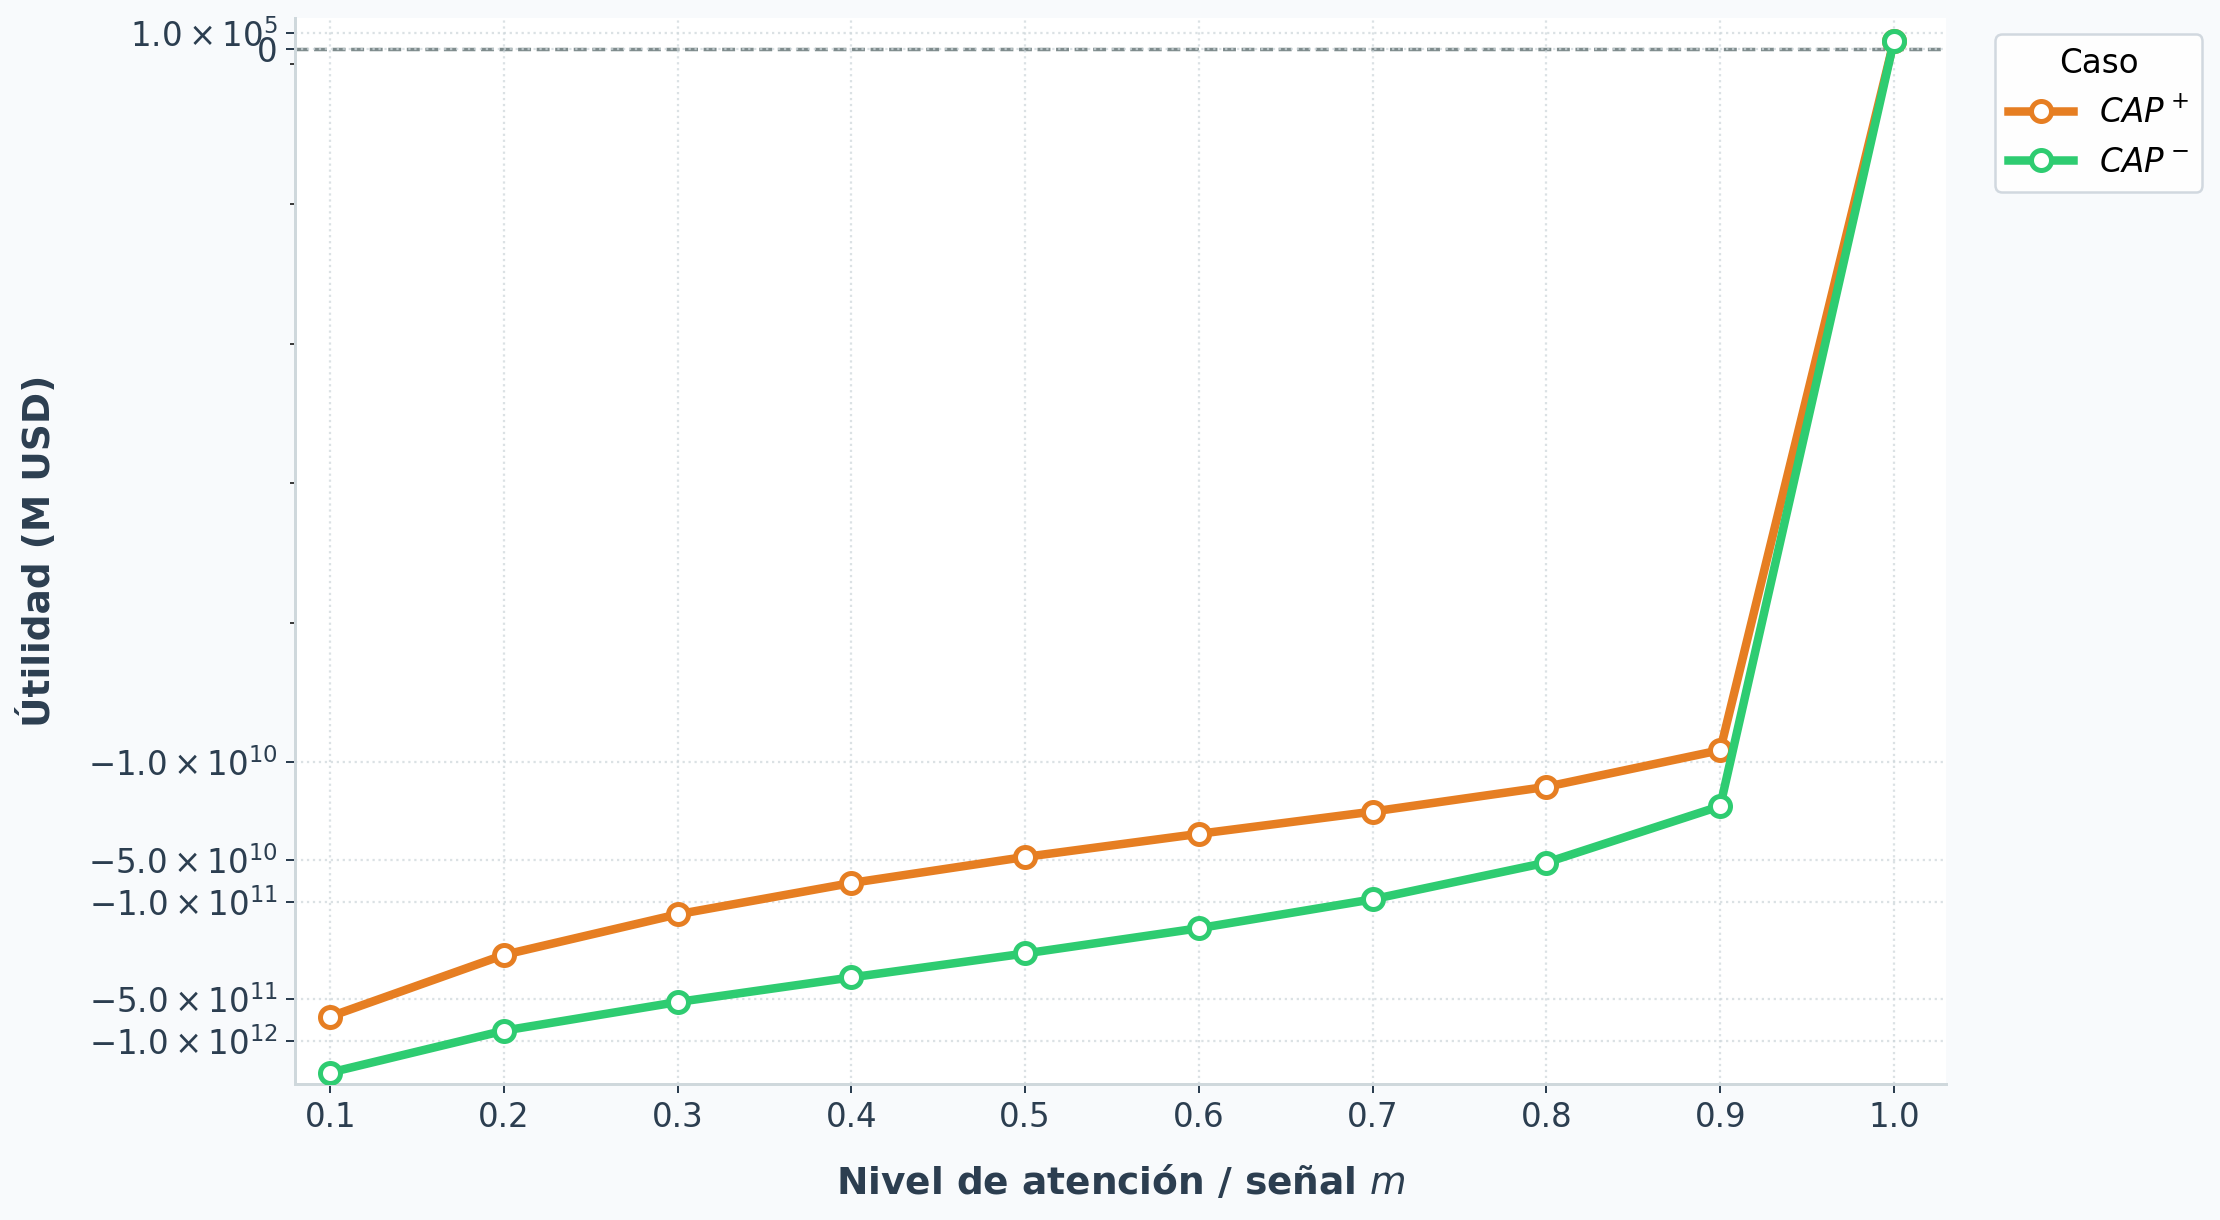
\includegraphics[
    width=0.98\textwidth,
    height=0.76\textheight,
    keepaspectratio
]{figures/perdidas.png}

\vspace{0.05cm}

{\tiny
\begin{tcolorbox}[
    colback=white,
    colframe=SoftBlue,
    arc=1.5mm,
    boxrule=0.5pt,
    hbox,
    left=2pt,
    right=2pt,
    top=1pt,
    bottom=1pt
]
\centering
\textbf{Fórmulas usadas:}
\(
\mathcal{V}(\theta, CAP)=\pi^{a}\theta-\frac{\kappa}{2}(\theta-CAP)^2
\qquad
CAP = CAP_s \pm \sigma_{\epsilon}
\)
\end{tcolorbox}
}

\end{frame}


% \centering

% \renewcommand{\arraystretch}{1.25}
% \setlength{\tabcolsep}{8pt}

% \begin{table}[H]
% \centering

% \begin{tabular}{c c c c}
% \toprule

% \multicolumn{2}{c}{\textbf{Caso límite}} &
% \textbf{$CAP_s + \sigma_\varepsilon$} &
% \textbf{$CAP_s - \sigma_\varepsilon$} \\

% \cmidrule(lr){1-2}
% \cmidrule(lr){3-3}
% \cmidrule(lr){4-4}

% \textbf{$m$} &
% \textbf{$\theta$ (MtCO$_2$e)} &
% \textbf{Beneficio (M USD)} &
% \textbf{Beneficio (M USD)} \\

% \midrule

% 0,0 & 311,0 & N/A & N/A \\

% 0,2 & 301,6 & $-2.40 \times 10^{14}$ & $-8.36 \times 10^{14}$ \\

% 0,4 & 292,3 & $-7.32 \times 10^{13}$ & $-3.47 \times 10^{14}$ \\

% 0,6 & 282,9 & $-3.25 \times 10^{13}$ & $-1.54 \times 10^{14}$ \\

% 0,8 & 273,6 & $-1.50 \times 10^{13}$ & $-5.23 \times 10^{13}$ \\

% 1,0 & 264,2 & $5.25 \times 10^{7}$ & $5.25 \times 10^{7}$ \\

% \bottomrule
% \end{tabular}

% \end{table}

% \end{frame}

\begin{frame}{Riesgo de Incertidumbre: Costo Social del Carbono}

\vspace{0.1cm}
\begin{columns}[T]
\begin{column}{0.32\textwidth}
\begin{tcolorbox}[tarjeta=DeepBlue, title={\faCloudRain\ \ Eventos extremos más frecuentes}]
{\scriptsize\begin{itemize}\setlength\itemsep{2pt}
\item Infraestructura \item Capital físico \item Actividad económica
\end{itemize}}
\end{tcolorbox}
\end{column}
\begin{column}{0.32\textwidth}
\begin{tcolorbox}[tarjeta=ClimateGreen, title={\faSeedling\ \ Sequías y cambios en el clima}]
{\scriptsize\begin{itemize}\setlength\itemsep{2pt}
\item Producción agrícola \item Oferta \item Precios
\end{itemize}}
\end{tcolorbox}
\end{column}
\begin{column}{0.32\textwidth}
\begin{tcolorbox}[tarjeta=SoftBlue, title={\faWater\ \ Daños en ecosistemas y recursos naturales}]
{\scriptsize\begin{itemize}\setlength\itemsep{2pt}
\item Agua \item Pesquerías \item Biodiversidad
\end{itemize}}
\end{tcolorbox}
\end{column}
\end{columns}

\end{frame}


\begin{frame}{Matriz energética 2030}

\centering
\vspace{-0.15cm}

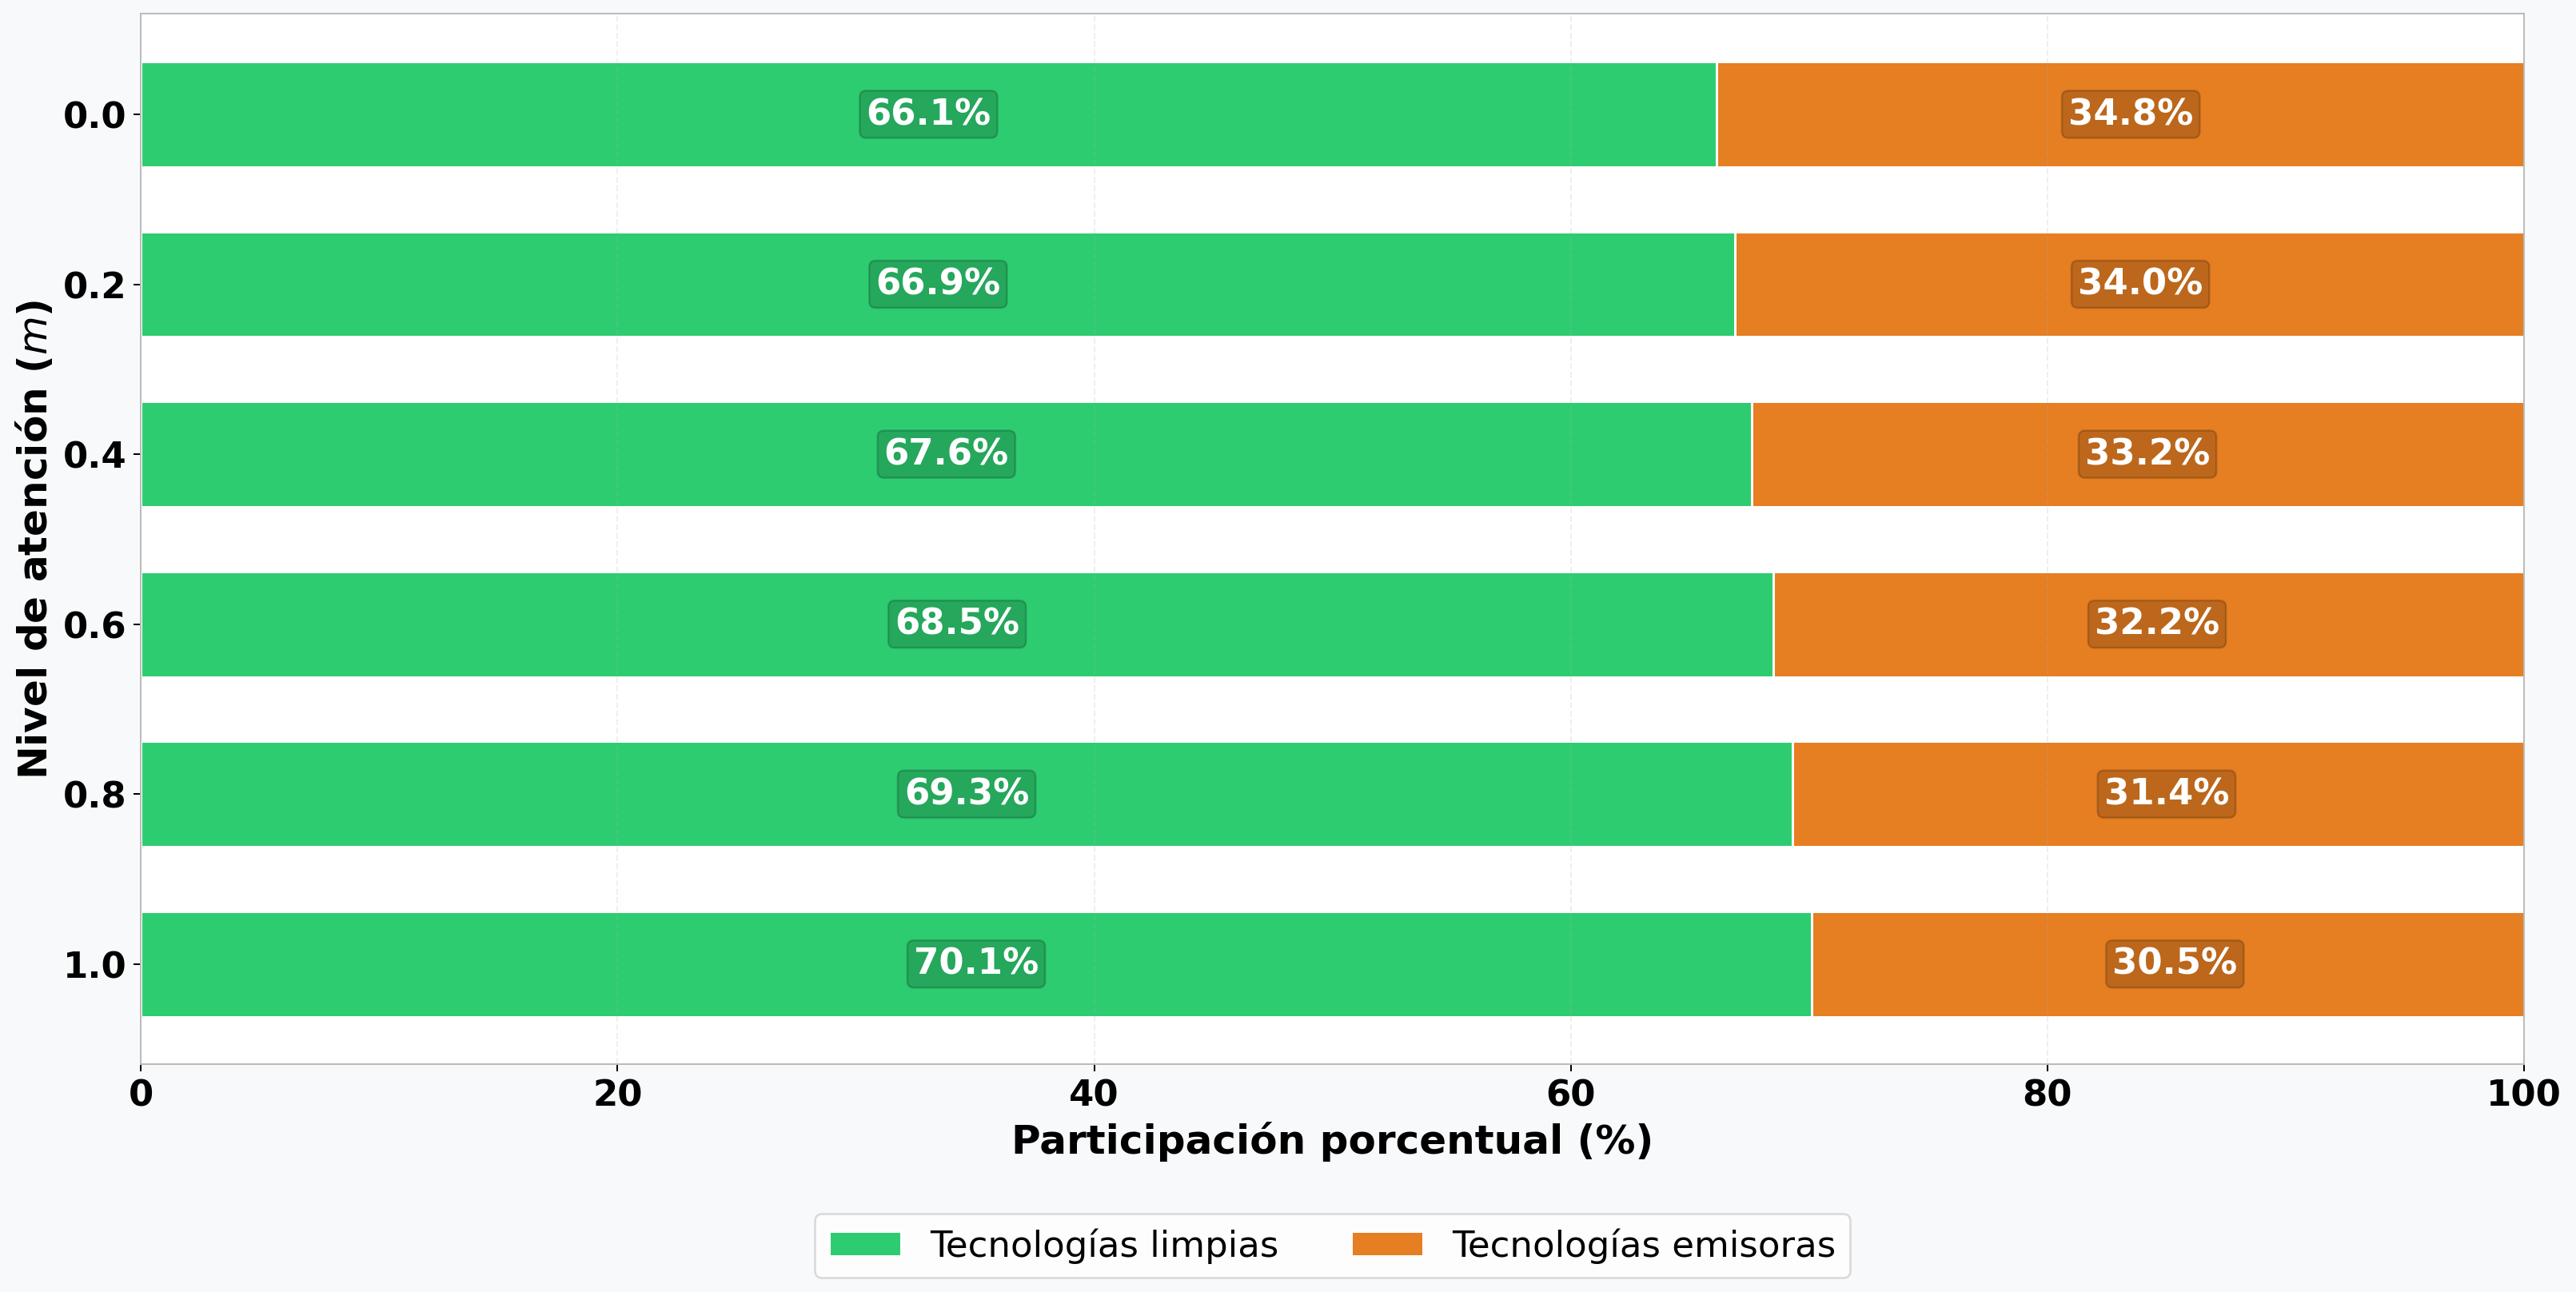
\includegraphics[
    width=0.98\textwidth,
    height=0.76\textheight,
    keepaspectratio
]{figures/melect3.png}

\vspace{0.05cm}

{\tiny
\begin{tcolorbox}[
    colback=white,
    colframe=SoftBlue,
    arc=1.5mm,
    boxrule=0.6pt,
    hbox,
    left=2pt,
    right=2pt,
    top=2pt,
    bottom=2pt
]
\centering
\textbf{Metodología:} 
$\% \, \mathrm{Fuente} = \frac{\mathrm{MWh\ Fuente}}{\mathrm{MWh\ Totales}} \times 100$
\end{tcolorbox}
}

\end{frame}



\begin{frame}{Conclusión}
\begin{figure}{}
    \centering
    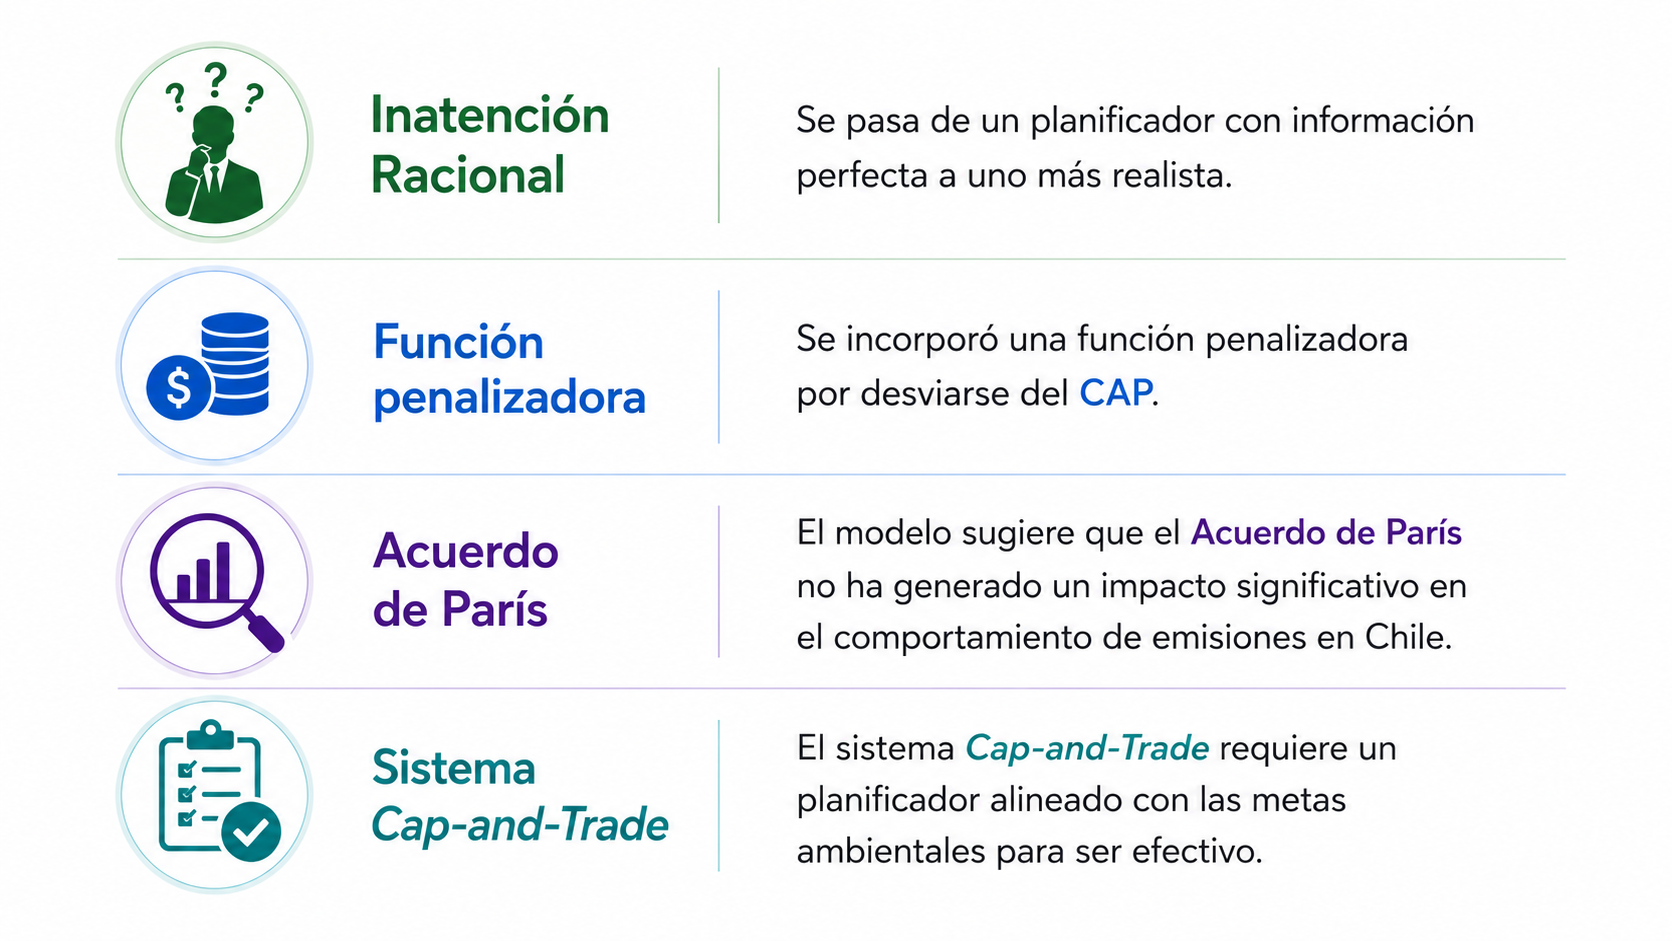
\includegraphics[
        width=1\linewidth,
        trim=15 15 15 15,
        clip
    ]{figures/conclusion.png}
\end{figure}

\end{frame}



\begin{frame}{}
    \begin{center}
        \textbf{\large ¡Muchas gracias por su atención!} \\
        \vspace{0.2cm}
    \end{center}
\end{frame}

\appendix

\begin{frame}[allowframebreaks]{Bibliografía}
    \bibliographystyle{apalike}
    \bibliography{references}
    Sector Energía: SNI Chile. Ministerio del Medio Ambiente. Disponible en: mma.gob.cl\\
    Plan de Descarbonización: Ministerio de Energía de Chile (2024). Plan de Descarbonización: Borrador para consulta pública.\\
    Precio Social del Carbono: Gobierno de Chile (2024). Actualizan precio social del carbono para incentivar la reducción de emisiones de CO2. Disponible en: www.gob.cl\\
\end{frame}
























\begin{frame}
    \titlepage
\end{frame}

\begin{frame}
    \vspace*{\fill} % Centrado vertical
    \begin{center}
        {\Huge \textbf{Anexos}}
        
        \vspace{0.4cm}
        \rule{3cm}{0.8pt} % Línea decorativa opcional para dar estilo
    \end{center}
    \vspace*{\fill}
\end{frame}

\begin{frame}{Planificador Social  \cite{amigo_two_2021}: función objetivo}
\small
El planificador elige $\theta$ considerando incertidumbre en el verdadero límite ambiental $CAP$:
\[
CAP \sim \mathcal{N}(\mu,\sigma^2)
\]

y debe asegurar que no lo exceda con alta probabilidad:
\[
\Pr(\theta \ge CAP) \le \epsilon
\]

\textbf{Problema a maximizar:}
\[
\max_{\theta} \ \theta\,\pi^a - \mathcal{F}(\theta)
\]

sujeto a la restricción probabilística:
\[
\varphi^{-1}(\epsilon)\,\sigma + \mu - \theta \ge 0
\]
\end{frame}
\begin{frame}{Escenario con costo fijo: $F(\theta) = 3$}
\begin{figure}[H]
\centering
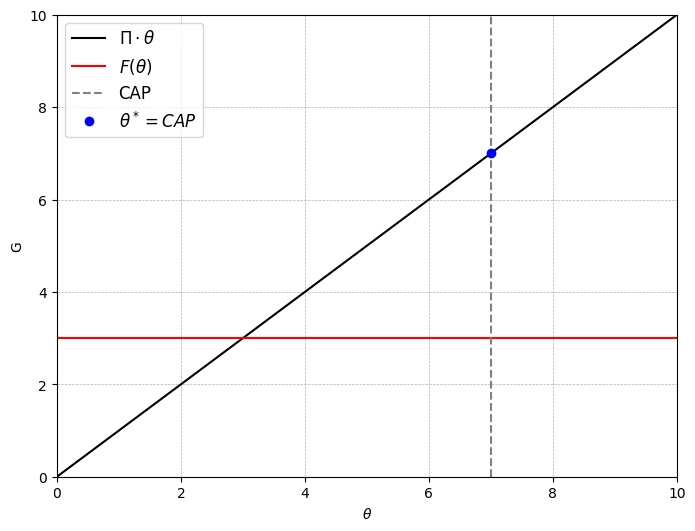
\includegraphics[width=0.75\linewidth]{figures/ejemplo_1.png}
\caption{Escenario con costo fijo: $F(\theta) = 3$}
\label{fig:ejemplo1}
\end{figure}
\end{frame}

\begin{frame}{Escenario con costo convexo: $F(\theta) = (\theta − 3)^2 + 1$}
    \begin{figure}[H]
    \centering    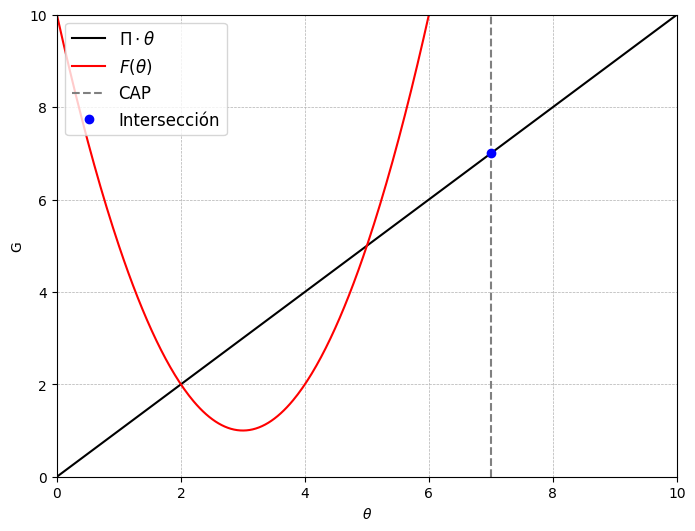
\includegraphics[width=0.75\linewidth]{figures/ejemplo_2.png}
    \caption{Escenario con costo convexo: $F(\theta) = (\theta − 3)^2 + 1$}
    \label{fig:ejemplo2}
    \end{figure}
\end{frame}




\begin{frame}{Modelo Profit-Oriented \cite{munoz_lhuillier_inversion_2022}}
\begin{align}
\max_{\theta, P} \quad & \theta \pi^{a} P - c(P-d)^{2} \label{eq:modelo_profit_obj} \\
\text{s.a.} \quad 
& \theta \pi^{a} P - c(P-d)^{2} \geq 0 \label{eq:restriccion_participacion} \\
& \theta \leq \hat{\theta} \label{eq:restriccion_theta_hat} \\
& 0 \leq P \leq 1 \label{eq:restriccion_precio} \\
& \theta \geq 0 \label{eq:restriccion_theta}
\end{align}

\end{frame}


\begin{frame}{Escenario con costo convexo: $F(\theta) = (\theta − 3)^2 + 1$}
    \begin{figure}[H]
    \centering    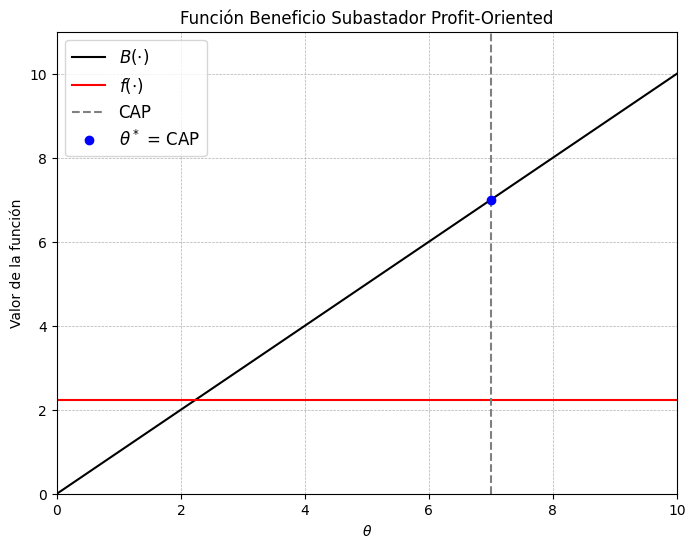
\includegraphics[width=0.75\linewidth]{figures/planificador social profit.png}
    \caption{Escenario con costo convexo: $F(\theta) = (\theta − 3)2 + 1$}
    \label{fig:ejemplo2}
    \end{figure}
\end{frame}

\begin{frame}{Modelo Profit-Oriented \cite{munoz_lhuillier_inversion_2022}}
\begin{align}
\max_{\theta, P} \quad & \theta \pi^{a} P - c(P-d)^{2} \label{eq:modelo_profit_obj} \\
\text{s.a.} \quad 
& \theta \pi^{a} P - c(P-d)^{2} \geq 0 \label{eq:restriccion_participacion} \\
& \theta \leq \hat{\theta} \label{eq:restriccion_theta_hat} \\
& 0 \leq P \leq 1 \label{eq:restriccion_precio} \\
& \theta \geq 0 \label{eq:restriccion_theta}
\end{align}
\end{frame}


\begin{frame}{Planificador Orientado al Bienestar Social}
    \begin{figure}[H]
    \centering    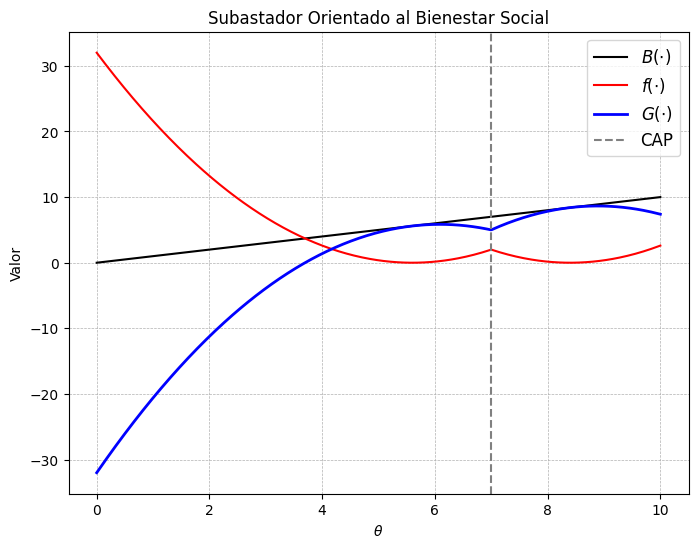
\includegraphics[width=0.75\linewidth]{figures/planificador social bienestar.png}
    \caption{}
    \label{fig:ejemplo2}
    \end{figure}
\end{frame}


% \begin{frame}{Limitación del modelo Profit-Oriented}

% \small

% \begin{itemize}

% \item Los ingresos aumentan linealmente con $\theta$.

% \vspace{0.2cm}

% \item El costo de información:
% \[
% c(P-d)^2
% \]
% no depende de $\theta$.

% \vspace{0.2cm}

% \item Emitir más permisos no genera una penalización adicional.

% \vspace{0.2cm}

% \item El óptimo económico termina siendo:
% \[
% \theta = CAP
% \]

% \end{itemize}

% \vspace{0.4cm}

% \begin{alertblock}{Inconsistencia}
% El modelo incorpora racionalidad limitada,
% pero mantiene incentivos a emitir la máxima cantidad posible.
% \end{alertblock}

% \end{frame}

% \begin{frame}{Limitación del modelo Welfare-Oriented}

% \small

% \begin{itemize}

% \item El modelo incorpora una penalización por desviarse del $CAP$.

% \vspace{0.2cm}

% \item Esto corrige parcialmente el problema del modelo Profit-Oriented.

% \vspace{0.2cm}

% \item Sin embargo, el beneficio:
% \[
% \theta \pi^a
% \]
% continúa creciendo con $\theta$.

% \vspace{0.2cm}

% \item Bajo ciertos parámetros, el óptimo puede ubicarse sobre el presupuesto ambiental:
% \[
% \theta > CAP
% \]

% \end{itemize}

% \vspace{0.4cm}

% \begin{alertblock}{Resultado observado}
% En la simulación:
% \[
% CAP = 7
% \qquad\text{y}\qquad
% \theta^* = 8.4
% \]

% El regulador sobre emite aproximadamente un 20\%.
% \end{alertblock}

% \end{frame}





\begin{frame}{Modelo Inatención Conductual}

\small

El planificador social enfrenta el siguiente problema:

\begin{align*}
\max_{\theta} \ \mathbb{E} \left[ 
\pi^a \theta - \frac{\kappa}{2}(\theta - CAP)^2 
\,\bigg|\, CAP_s \right]
\end{align*}

Derivando respecto a $\theta$:

\begin{align*}
0 
&= \frac{\partial}{\partial \theta}
\mathbb{E} \left[ 
\pi^a \theta - \frac{\kappa}{2}(\theta - CAP)^2 
\,\bigg|\, CAP_s \right] \\
&= \mathbb{E} \left[ 
\pi^a - \kappa(\theta - CAP) 
\,\bigg|\, CAP_s \right] \\
&= \pi^a - \kappa \theta + \kappa \mathbb{E}[CAP \mid CAP_s]
\end{align*}

\end{frame}





\begin{frame}{Modelo Inatención Conductual}

\small

Despejando:

\begin{align*}
\theta^*(CAP_s) 
= \mathbb{E}[CAP \mid CAP_s] + \frac{\pi^a}{\kappa}
\end{align*}

Siguiendo inatención conductual:

\begin{align*}
\mathbb{E}[CAP \mid CAP_s] 
= m\,CAP_s + (1-m)\,CAP_d
\end{align*}

Finalmente:

\begin{align*}
\boxed{
\theta^*(CAP_s) 
= m\,CAP_s + (1-m)\,CAP_d + \frac{\pi^a}{\kappa}
}
\end{align*}

\end{frame}


\begin{frame}{Variables y Parámetros del Modelo}
    \vspace{0.3cm}
    \centering
    \footnotesize % Reducimos un poco el tamaño para que respire la diapositiva
    \renewcommand{\arraystretch}{1.2} % Da un poco más de espacio vertical entre filas
    
    \begin{tabular}{ll c} % l=izq, l=izq, c=centro
        \hline
        \textbf{Símbolo} & \textbf{Descripción} & \textbf{Unidad} \\ \hline
        $\kappa$ & Costo social por desviación del $CAP$ & USD/tCO$_2$e \\
        $CAP_s$ & Señal observada (presupuesto percibido) & tCO$_2$e \\
        $CAP_d$ & Presupuesto por defecto (anclaje) & tCO$_2$e \\
        $\sigma_\epsilon^2$ & Varianza del error de percepción (ruido) & (tCO$_2$e)$^2$ \\
        $\sigma_{\text{CAP}}^2$ & Varianza del presupuesto real & (tCO$_2$e)$^2$ \\ \hline
    \end{tabular}

    \vspace{0.6cm}
    \begin{itemize}
        \item \scriptsize Los valores de $\sigma^2$ determinan el nivel de atención $m$ del planificador.
    \end{itemize}
\end{frame}



\begin{frame}{Estimaciones de CAP (1/2)}

\scriptsize

\begin{tabular}{l c c c}
\toprule
\textbf{Fuente} & \textbf{Fecha} & \textbf{CAP (MtCO$_2$e)} & \textbf{Horizonte} \\
\midrule
\cite{amigo_two_2021} & 10/02/2021 & 365,29 & 2019--2030 \\
\cite{ministerio_del_medio_ambiente_anteproyecto_2025} & 2025 & 300,27 & 2031--2035 \\
\cite{ministerio_del_medio_ambiente_reporte_2024} & 2024 & 332,34 & 2020--2022 \\
\cite{ministerio_del_medio_ambiente_reporte_2024} & 2024 & 296,67 & 2023--2030 \\
\cite{ministerio_de_energia_de_chile_plan_2024} & 2024 & 296,00 & 2020--2030 \\
\cite{gobierno_de_chile_estrategia_2021} & 21/10/2021 & 306,40 & 2020--2030 \\
\addlinespace
Climate Action Tracker & 02/11/2016 & 493,30 & 2030 \\
Climate Action Tracker & 06/11/2017 & 496,37 & 2030 \\
Climate Action Tracker & 23/03/2018 & 392,19 & 2030 \\
Climate Action Tracker & 16/08/2018 & 401,38 & 2030 \\
Climate Action Tracker & 30/11/2018 & 407,51 & 2030 \\
Climate Action Tracker & 01/11/2018 & 364,62 & 2020 \\
\bottomrule
\end{tabular}

\end{frame}

\begin{frame}{Estimaciones de CAP (2/2)}

\scriptsize
\begin{center}
    \begin{tabular}{l c c c}
    \toprule
    \textbf{Fuente} & \textbf{Fecha} & \textbf{CAP (MtCO$_2$e)} & \textbf{Horizonte} \\
    \midrule
    Climate Action Tracker & 02/12/2019 & 318,24 & 2020--2030 \\
    Climate Action Tracker & 19/09/2019 & 401,38 & 2030 \\
    Climate Action Tracker & 19/09/2019 & 373,81 & 2020 \\
    Climate Action Tracker & 02/12/2019 & 297,21 & 2030 \\
    Climate Action Tracker & 04/11/2022 & 286,76 & 2020--2030 \\
    Climate Action Tracker & 03/11/2025 & 294,14 & 2031--2035 \\
    \addlinespace
    Climate Action Tracker (CFI) & 02/11/2016 & 422,83 & 2030 \\
    Climate Action Tracker (CFI) & 06/11/2017 & 427,43 & 2030 \\
    Climate Action Tracker (CFI) & 23/03/2018 & 333,98 & 2030 \\
    Climate Action Tracker (CFI) & 16/08/2018 & 344,70 & 2030 \\
    Climate Action Tracker (CFI) & 30/11/2018 & 350,83 & 2030 \\
    Climate Action Tracker (CFI) & 19/09/2019 & 344,70 & 2030 \\
    Climate Action Tracker (CFI) & 04/11/2022 & 283,42 & 2030 \\
    Climate Action Tracker (CFI) & 07/10/2024 & 280,36 & 2030 \\
    \addlinespace
    \cite{palma_behnke_chilean_2019} & 2019 & 300,94 & 2020--2030 \\
    \bottomrule
    \end{tabular}

    \vspace{0.2cm}
    \tiny
    \textbf{Nota:} CFI = considerando financiamiento internacional. 
    Climate Action Tracker: \url{https://climateactiontracker.org/}.
\end{center}
\end{frame}







\begin{frame}{$\theta_{base}$ según atención}

\centering

\small % Reduce tamaño general de la tabla

\renewcommand{\arraystretch}{1.05}
\setlength{\tabcolsep}{8pt}

\begin{tabular}{c c c}
\toprule
\textbf{$\sigma_{\varepsilon}$} & \textbf{$m$} & \textbf{$\theta_{base}$} \\
\textbf{(MtCO$_2$e)} & & \textbf{(MtCO$_2$e)} \\
\midrule
$\infty$ & 0,0 & 311,01 \\
185,58 & 0,1 & 306,33 \\
123,72 & 0,2 & 301,65 \\
94,49  & 0,3 & 296,97 \\
75,76  & 0,4 & 292,29 \\
61,86  & 0,5 & 287,61 \\
50,51  & 0,6 & 282,93 \\
40,50  & 0,7 & 278,24 \\
30,93  & 0,8 & 273,56 \\
20,62  & 0,9 & 268,88 \\
0,00   & 1,0 & 264,20 \\
\bottomrule
\end{tabular}

\vspace{0.25cm}

\footnotesize{Fuente: Elaboración propia.}

\end{frame}

\begin{frame}{Calibración del Modelo sobre la Matriz eléctrica - año 2024}
    \begin{table}[H]
\centering
\small
\label{tab:top10_distancia_mix}
\renewcommand{\arraystretch}{1.1}
\setlength{\tabcolsep}{6pt}
\begin{tabular}{c c c}
\toprule
\textbf{$\sigma_{\varepsilon}$ (MtCO$_2$e)} & \textbf{$m$} & \textbf{Distancia absoluta} \\
\midrule
$\infty$ & 0,0 & 0,2727 \\
185,58 & 0,1 & 0,2758 \\
123,72 & 0,2 & 0,2788 \\
94,49  & 0,3 & 0,2818 \\
75,76  & 0,4 & 0,2849 \\
61,86  & 0,5 & 0,2879 \\
50,51  & 0,6 & 0,2909 \\
40,50  & 0,7 & 0,2940 \\
30,93  & 0,8 & 0,2970 \\
20,62  & 0,9 & 0,2998 \\
0,00   & 1,0 & 0,3026 \\
\bottomrule
\end{tabular}

\vspace{0.15cm}
\footnotesize{Fuente: Elaboración propia.}
\end{table}
\end{frame}











% --- DIAPOSITIVA 3: EVOLUCIÓN DE LA MATRIZ ENERGÉTICA ---

\begin{frame}{Resultados Caso Borde $CAP+\epsilon$}
\begin{table}[H]
\centering
\label{tab:resultados_m}
\renewcommand{\arraystretch}{1.2}
\setlength{\tabcolsep}{3pt} % Reduce espacio entre columnas para ganar ancho

\resizebox{\textwidth}{!}{% Ajusta la tabla al ancho de la diapositiva
\begin{tabular}{ccccc}
\toprule
$m$ & CAP (MtCO$_2$) & $\theta-CAP$ (MtCO$_2$) & Costo (M USD) & Beneficio (M USD) \\
\midrule
0,0 & N/A & N/A & N/A & N/A \\
0,1 & 449,78 & -143,45 & 662.589.589.804,07 & -662.589.533.175,84 \\
0,2 & 387,92 & -86,27 & 239.644.999.121,04 & -239.644.942.893,35 \\
0,3 & 358,69 & -61,72 & 122.674.630.993,48 & -122.674.575.181,06 \\
0,4 & 339,96 & -47,67 & 73.186.603.953,91 & -73.186.548.571,17 \\
0,5 & 326,06 & -38,45 & 47.612.752.798,72 & -47.612.697.859,80 \\
0,6 & 314,71 & -31,78 & 32.527.377.488,24 & -32.527.323.007,85 \\
0,7 & 304,70 & -26,45 & 22.532.072.038,36 & -22.532.018.030,91 \\
0,8 & 295,13 & -21,57 & 14.977.809.285,24 & -14.977.755.754,22 \\
0,9 & 284,82 & -15,94 & 8.180.115.598,42 & -8.180.062.570,72 \\
1,0 & 264,20 & 0,00 & 0,00 & 52.510,01 \\
\bottomrule
\end{tabular}%
}
\end{table}
\end{frame}

\begin{frame}{Resultados Caso Borde $CAP-\epsilon$}
\begin{table}[H]
\centering
\label{tab:resultados_m_2}
\renewcommand{\arraystretch}{1.2}
\setlength{\tabcolsep}{3pt}

\resizebox{\textwidth}{!}{%
\begin{tabular}{ccccc}
\toprule
$m$ & CAP (MtCO$_2$) & $\theta-CAP$ (MtCO$_2$) & Costo (M USD) & Beneficio (M USD) \\
\midrule
0,0 & N/A & N/A & N/A & N/A \\
0,1 & 78,62 & 227,71 & 1.669.659.335.377,53 & -1.669.659.278.749,30 \\
0,2 & 140,48 & 161,17 & 836.427.074.998,41 & -836.427.018.770,71 \\
0,3 & 169,71 & 127,26 & 521.499.495.445,26 & -521.499.439.632,84 \\
0,4 & 188,44 & 103,85 & 347.276.282.042,91 & -347.276.226.660,18 \\
0,5 & 202,34 & 85,27 & 234.107.160.573,50 & -234.107.105.634,59 \\
0,6 & 213,69 & 69,23 & 154.345.018.699,95 & -154.344.964.219,57 \\
0,7 & 223,70 & 54,54 & 95.785.627.884,60 & -95.785.573.877,16 \\
0,8 & 233,27 & 40,29 & 52.276.698.090,68 & -52.276.644.559,66 \\
0,9 & 243,58 & 25,30 & 20.613.082.650,14 & -20.613.029.622,44 \\
1,0 & 264,20 & 0,00 & 0,00 & 52.510,01 \\
\bottomrule
\end{tabular}%
}
\vspace{0.2cm}
\begin{flushleft}
\footnotesize Fuente: Elaboración propia.
\end{flushleft}
\end{table}
\end{frame}



\begin{frame}{Evolución de la Matriz Energética (m=1, 2020-2030)}
    \centering
    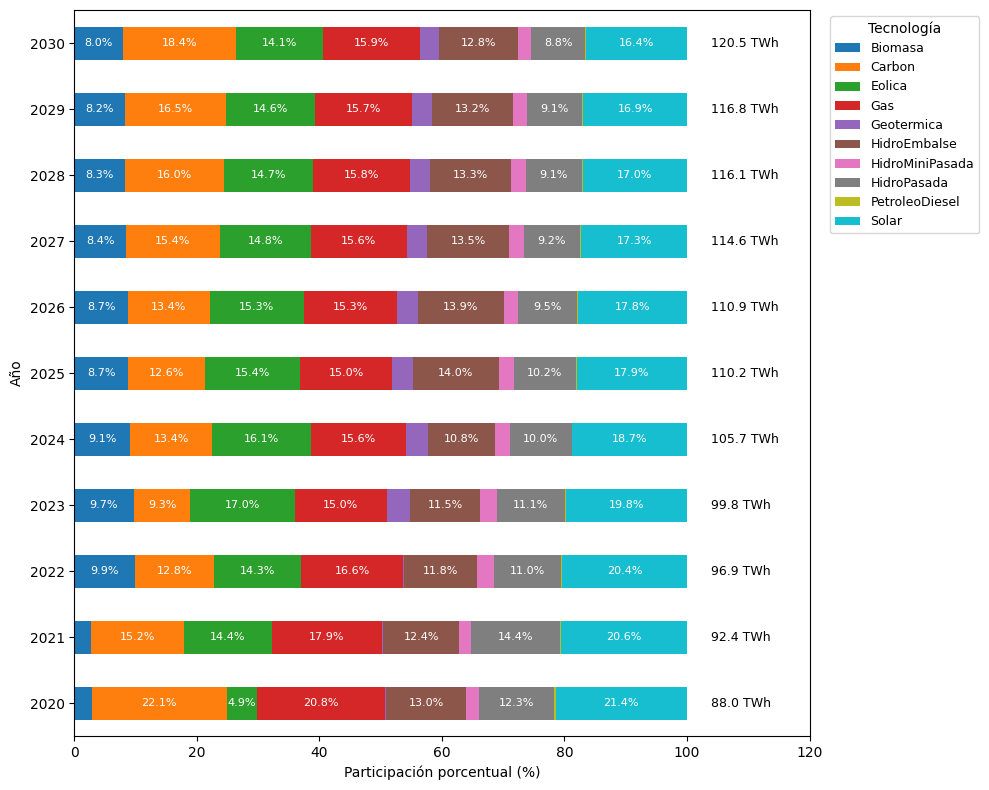
\includegraphics[width=\textwidth,height=0.9\textheight,keepaspectratio]{figures/mprx0.0.png}
 
\end{frame}

\begin{frame}[fragile]{Definición de $\theta$ según nivel de atención}

\small

\begin{block}{Código en Julia}
\begin{verbatim}
k = 64.4

# m = 0.0
theta_base = 311_013_377.53
.
.
.
# m = 1.0
# theta_base = 264_200_000.00

@expression(model, theta, theta_base + pi_a / k)
\end{verbatim}
\end{block}

\vspace{0.2cm}

\footnotesize{
Cada valor de \texttt{theta\_base} representa el nivel base de permisos
asociado a un nivel de atención \(m\).
}
\end{frame}


%====================================================
% ANEXOS: Parámetros originales de Amigo et al. (2021)
%====================================================

\section{Parámetros originales de Amigo et al. (2021)}

%----------------------------------------------------
\begin{frame}{Factores de planta por tecnología}

\centering

\renewcommand{\arraystretch}{1.15}
\setlength{\tabcolsep}{12pt}

\begin{table}
\centering
\small
\begin{tabular}{l c}
\toprule
\textbf{Tecnología} & \textbf{Factor de planta (CF)} \\
\midrule
Biomasa           & 0.55 \\
Carbón            & 0.99 \\
Eólica            & 0.23 \\
Gas               & 0.60 \\
Geotérmica        & 0.65 \\
Hidro Embalse     & 0.39 \\
Hidro Pasada      & 0.43 \\
Hidro Mini Pasada & 0.39 \\
Petróleo Diésel   & 0.90 \\
Solar             & 0.24 \\
\bottomrule
\end{tabular}
\end{table}

\vspace{0.15cm}

{\footnotesize Fuente: Amigo et al. (2021).}

\end{frame}

%----------------------------------------------------
\begin{frame}{Anexo: Costos de inversión por tecnología}

\centering

\renewcommand{\arraystretch}{1.15}
\setlength{\tabcolsep}{12pt}

\begin{table}
\centering
\small
\begin{tabular}{l c}
\toprule
\textbf{Tecnología} & \textbf{Costo de inversión (USD/kW)} \\
\midrule
Biomasa            & 3\,253 \\
Carbón             & 3\,000 \\
Eólica             & 1\,361 \\
Gas                & 800 \\
Geotérmica         & 5\,870 \\
Hidro Embalse      & 2\,180 \\
Hidro Pasada       & 4\,050 \\
Hidro Mini Pasada  & 3\,565 \\
Petróleo Diésel    & 687 \\
Solar              & 2\,000 \\
\bottomrule
\end{tabular}
\end{table}

\vspace{0.15cm}

{\footnotesize Fuente: elaboración propia en base al trabajo de Amigo et al. (2021).}

\end{frame}

%----------------------------------------------------
\begin{frame}{Anexo: Factores de emisión por tecnología}

\centering

\renewcommand{\arraystretch}{1.15}
\setlength{\tabcolsep}{12pt}

\begin{table}
\centering
\small
\begin{tabular}{l c}
\toprule
\textbf{Tecnología} & \textbf{Factor de emisión $\epsilon_i$ (tCO$_2$e/MWh)} \\
\midrule
Biomasa            & 0.00 \\
Carbón             & 0.91 \\
Eólica             & 0.00 \\
Gas                & 0.65 \\
Geotérmica         & 0.00 \\
Hidro Embalse      & 0.00 \\
Hidro Pasada       & 0.00 \\
Hidro Mini Pasada  & 0.00 \\
Petróleo Diésel    & 0.91 \\
Solar              & 0.00 \\
\bottomrule
\end{tabular}
\end{table}

\vspace{0.15cm}

{\footnotesize Fuente: elaboración propia en base al trabajo de Amigo et al. (2021).}

\end{frame}
\end{document}


